%% \documentclass[preprint,5p,times,twocolumn,authoryear]{elsarticle}

%% Use the option review to obtain double line spacing
\documentclass[preprint,review,12pt,authoryear]{elsarticle}

%% Use the options 1p,twocolumn; 3p; 3p,twocolumn; 5p; or 5p,twocolumn
%% for a journal layout:
%% \documentclass[final,1p,times]{elsarticle}
%% \documentclass[final,1p,times,twocolumn]{elsarticle}
%% \documentclass[final,3p,times]{elsarticle}
%% \documentclass[final,3p,times,twocolumn]{elsarticle}
%% \documentclass[final,5p,times]{elsarticle}
%% \documentclass[final,5p,times,twocolumn]{elsarticle}

%% For including figures, graphicx.sty has been loaded in
%% elsarticle.cls. If you prefer to use the old commands
%% please give \usepackage{epsfig}

%% The amssymb package provides various useful mathematical symbols
\usepackage{amssymb}
\usepackage{amsmath}
\usepackage{latexsym}     
\usepackage{hyperref}
\usepackage{subcaption}
\usepackage{lineno}
\usepackage[margin=1in]{geometry}   

\usepackage{pstricks}
\usepackage{tikz} %required for wire diagram
\usetikzlibrary{shapes.geometric, arrows}
\usetikzlibrary{arrows,arrows.meta}
\usetikzlibrary{positioning} 
\usepackage{pst-node}
% add the following two lines to your document to get bigger arrows
\usetikzlibrary{arrows.meta}
\tikzset{>={Latex[width=3mm,length=3mm]}}
%% The amsthm package provides extended theorem environments
%% \usepackage{amsthm}

%% The lineno packages adds line numbers. Start line numbering with
%% \begin{linenumbers}, end it with \end{linenumbers}. Or switch it on
%% for the whole article with \linenumbers.
%% \usepackage{lineno}

\def\ds{\displaystyle}

\journal{Ecological Modeling}

\begin{document}

\linenumbers
\begin{frontmatter}


\title{An integral projection model for gizzard shad (\emph{Dorosoma cepedianum}) utilizing density-dependent age-0 survival}

\author{ J. Peirce$^{\rm 1,4}$,  G.  Sandland$^{\rm 3,4}$, B. Bennie$^{\rm 1}$, R.A. Erickson$^{\rm 2}$}
\address{
${\rm 1}$ University of Wisconsin - La Crosse, Mathematics \& Statistics Department\\ 
${\rm 2}$ U.S.G.S. Upper Mississippi Environmental Science Center\\ 
${\rm 3}$ University of Wisconsin - La Crosse, Biology Department\\
${\rm 4}$ River Studies Center} 

\begin{abstract}
%% Text of abstract
Gizzard shad (\emph{Dorosoma cepedianum}) are a common freshwater fish throughout the central and eastern portions of North America. 
Within these areas, gizzard shad play a number of critical roles in the freshwater community. 
Because of this, it is important that we understand how gizzard shad populations respond to environmental changes and what these changes may mean for aquatic communities in general and fish assemblages in particular. 
Here we introduce an integral projection model for gizzard shad based on empirical data and include density-dependent survival in age-0 fish. 
Integral projection models (IPM) are a generalization of stage-based, matrix population models that have been used to describe a wide range of organisms. 
IPMs are a natural choice for gizzard shad since many aspects of their life cycle have been studied. 
In this paper, we compared model outcomes to empirical patterns reported for this fish species at a key location along the Illinois River. 
Results of our work suggest that this model could serve as an important tool for predicting gizzard shad population responses to changing environmental conditions, including those mediated through species invasions.
\end{abstract}

%%Graphical abstract
\begin{graphicalabstract}
\begin{figure*}
\label{llife_cycle}
    \begin{center}
%\scalebox{.75}[.75]{
\begin{tikzpicture}[->,>=stealth',shorten >=1pt,auto,node distance=3cm,
  thick,
  main node/.style={rectangle,draw},
  box/.style = {draw=gray, very thick,
                            minimum height=11mm, text width=11mm, 
                            align=center},]
                              
\node[main node, align=center] (census_pres) at (0,3) {Census $t$ \\
        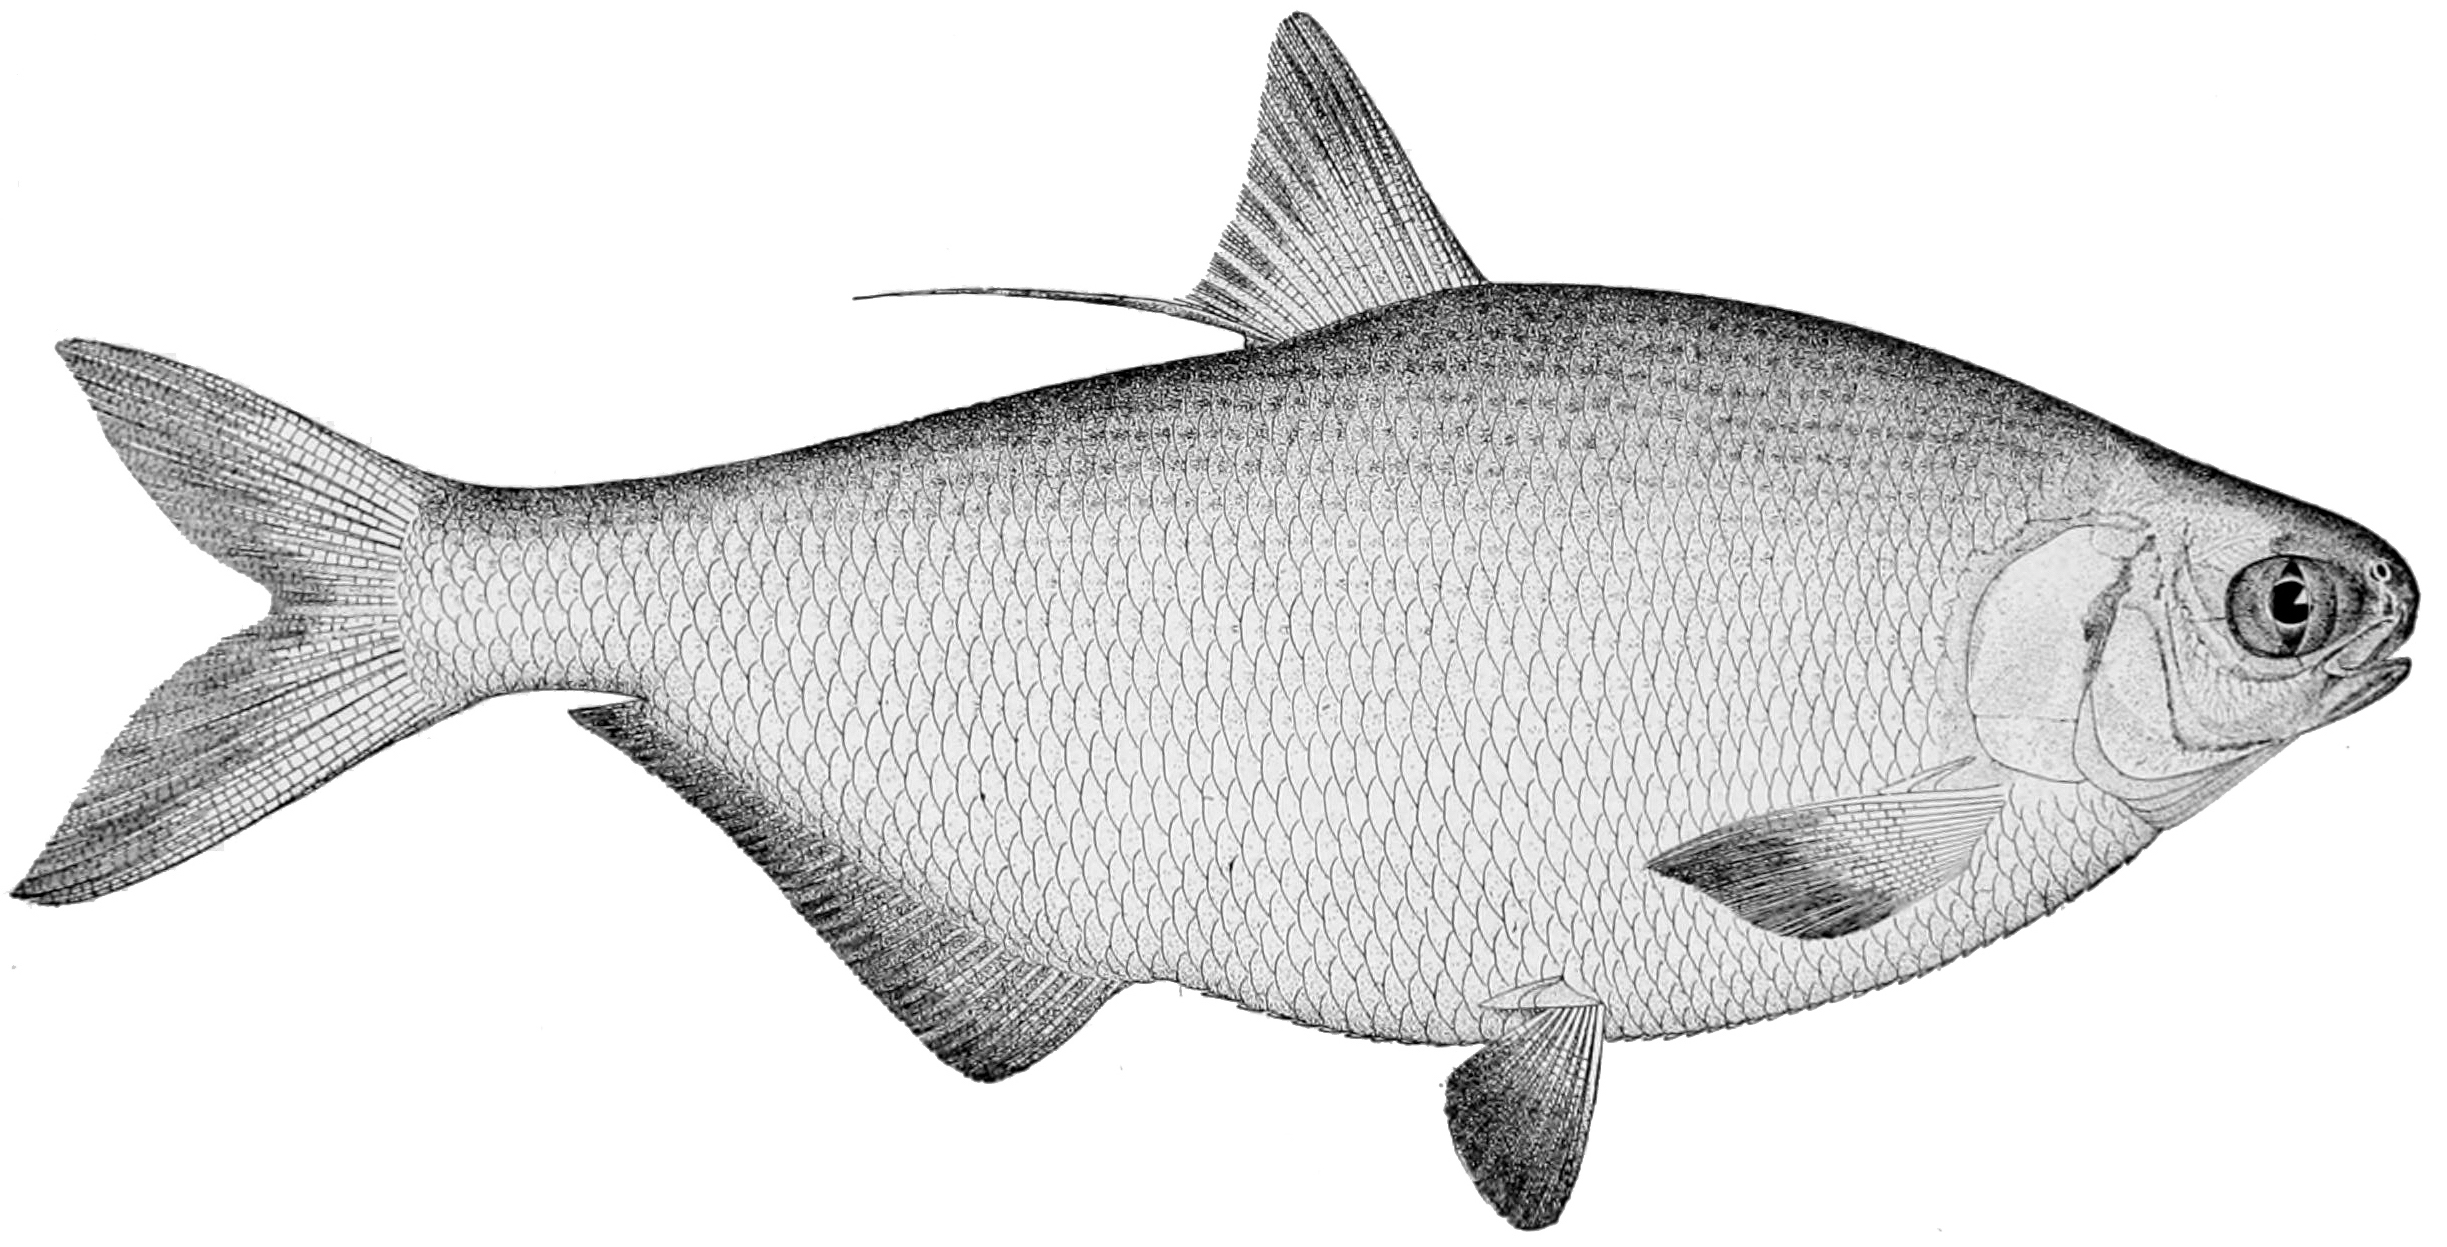
\includegraphics[width=0.12\textwidth]{adult.jpeg} \\
        $n(z,t)$};
\node[align=center] (repro) at (3.25,3) {Reproduction\\
        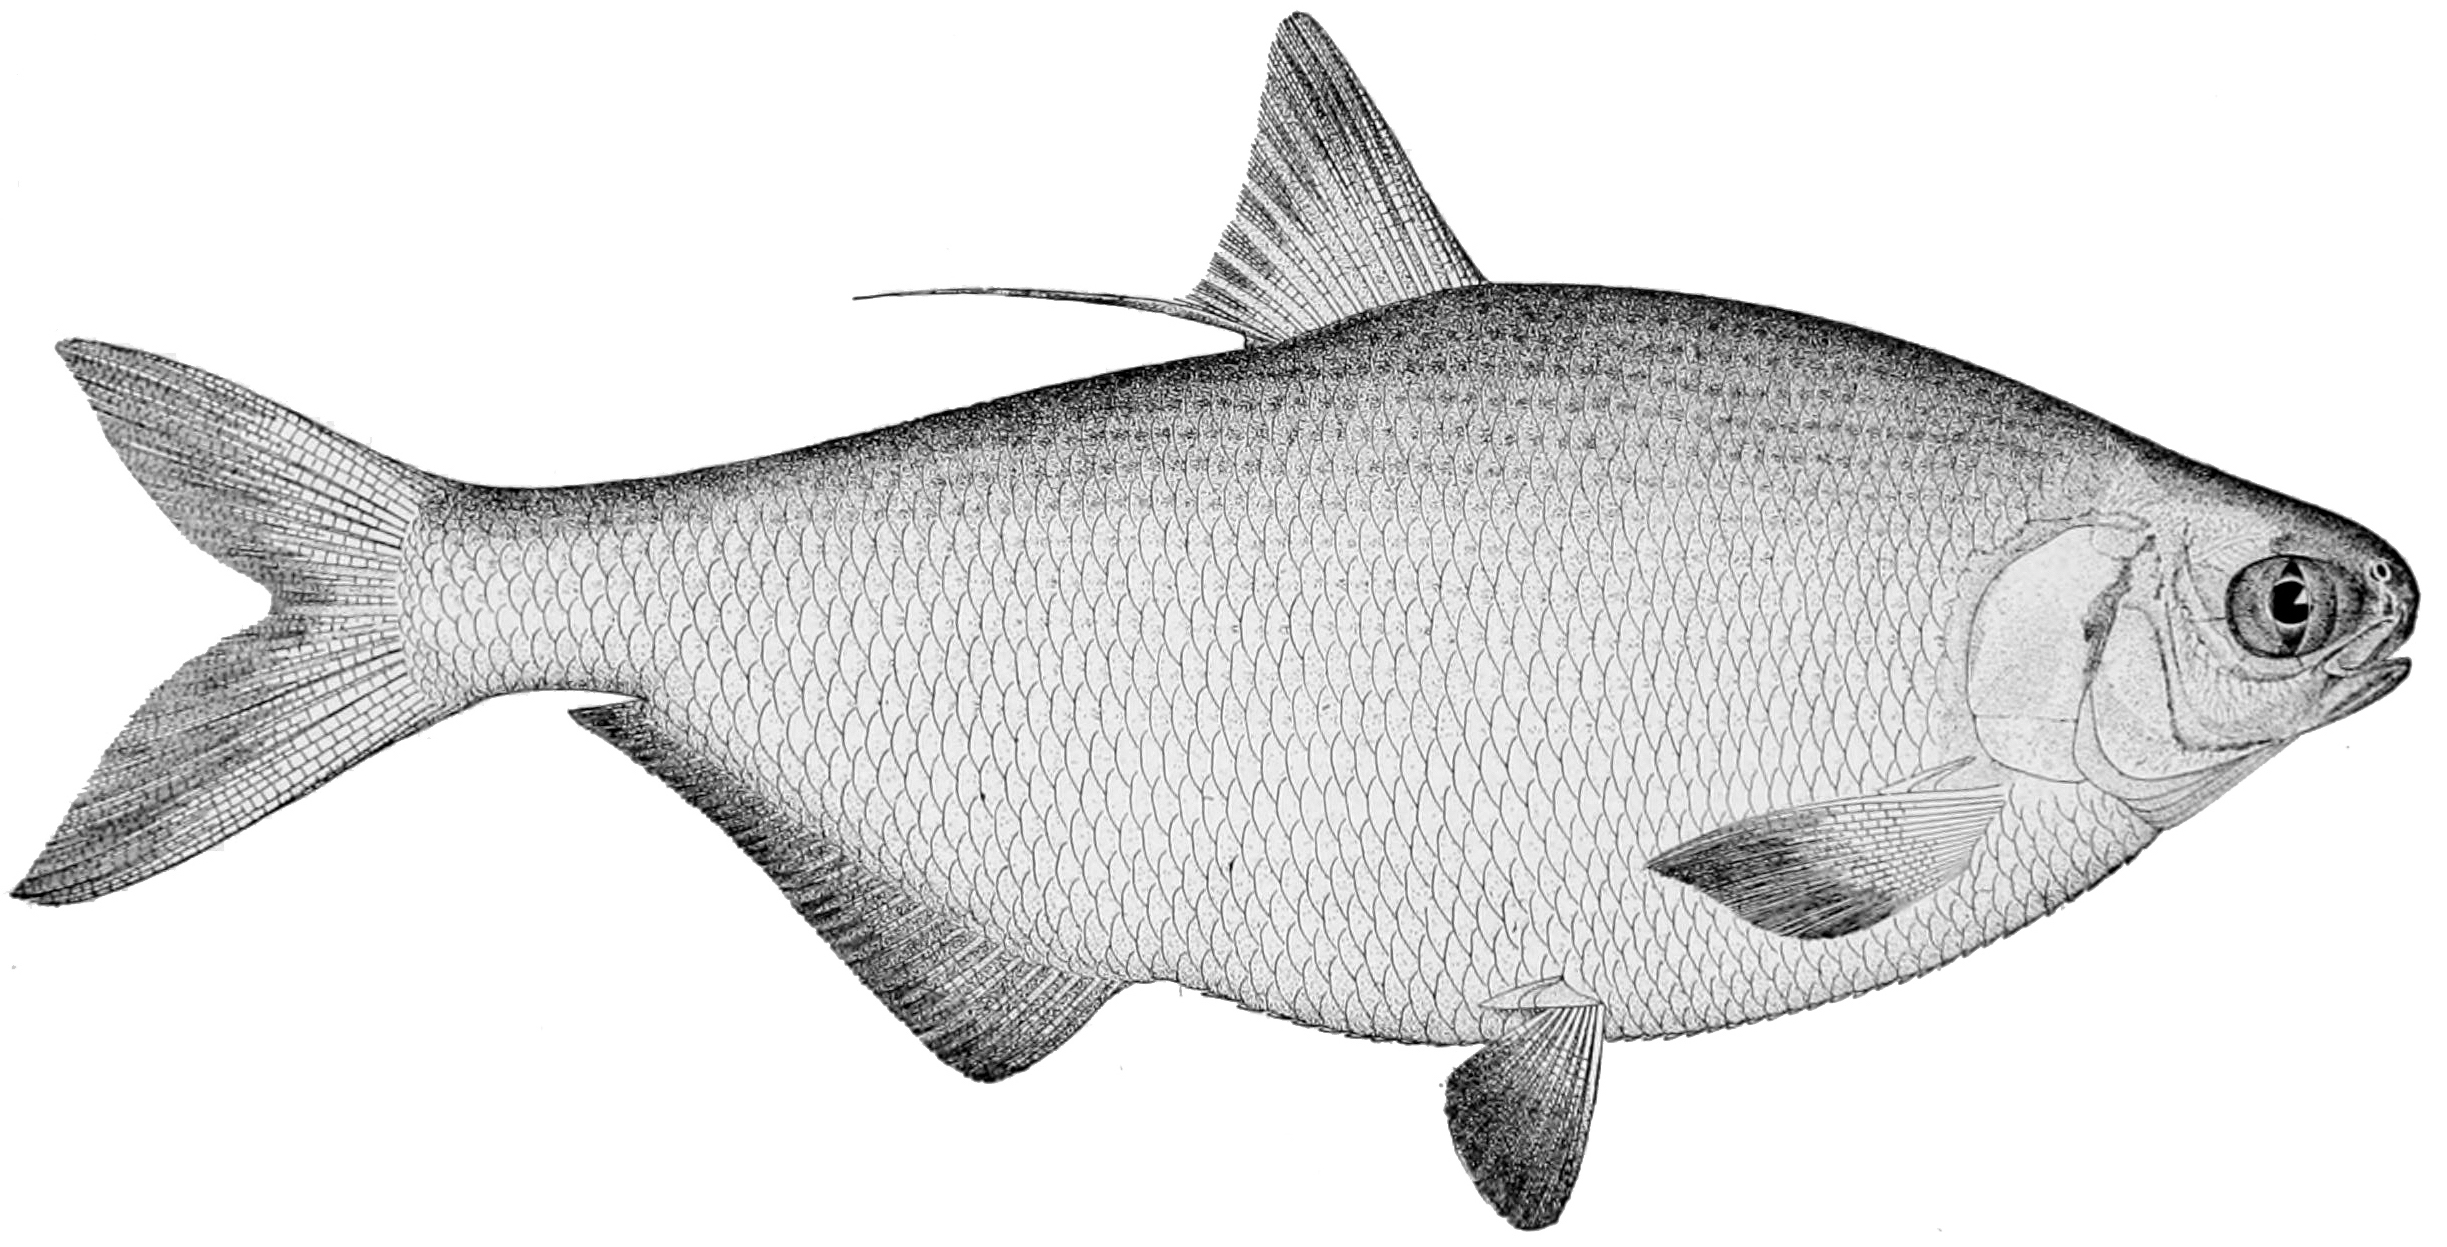
\includegraphics[width=0.12\textwidth]{adult.jpeg}\\
        };
\node (repro_in) at (2.3, 3)  {};
\node (repro_out) at (4.25, 3)  {};
\node (repro_down) at (3, 2.5)  {};
%\node[align=center] (surv) at (4.5,3) {\\
%        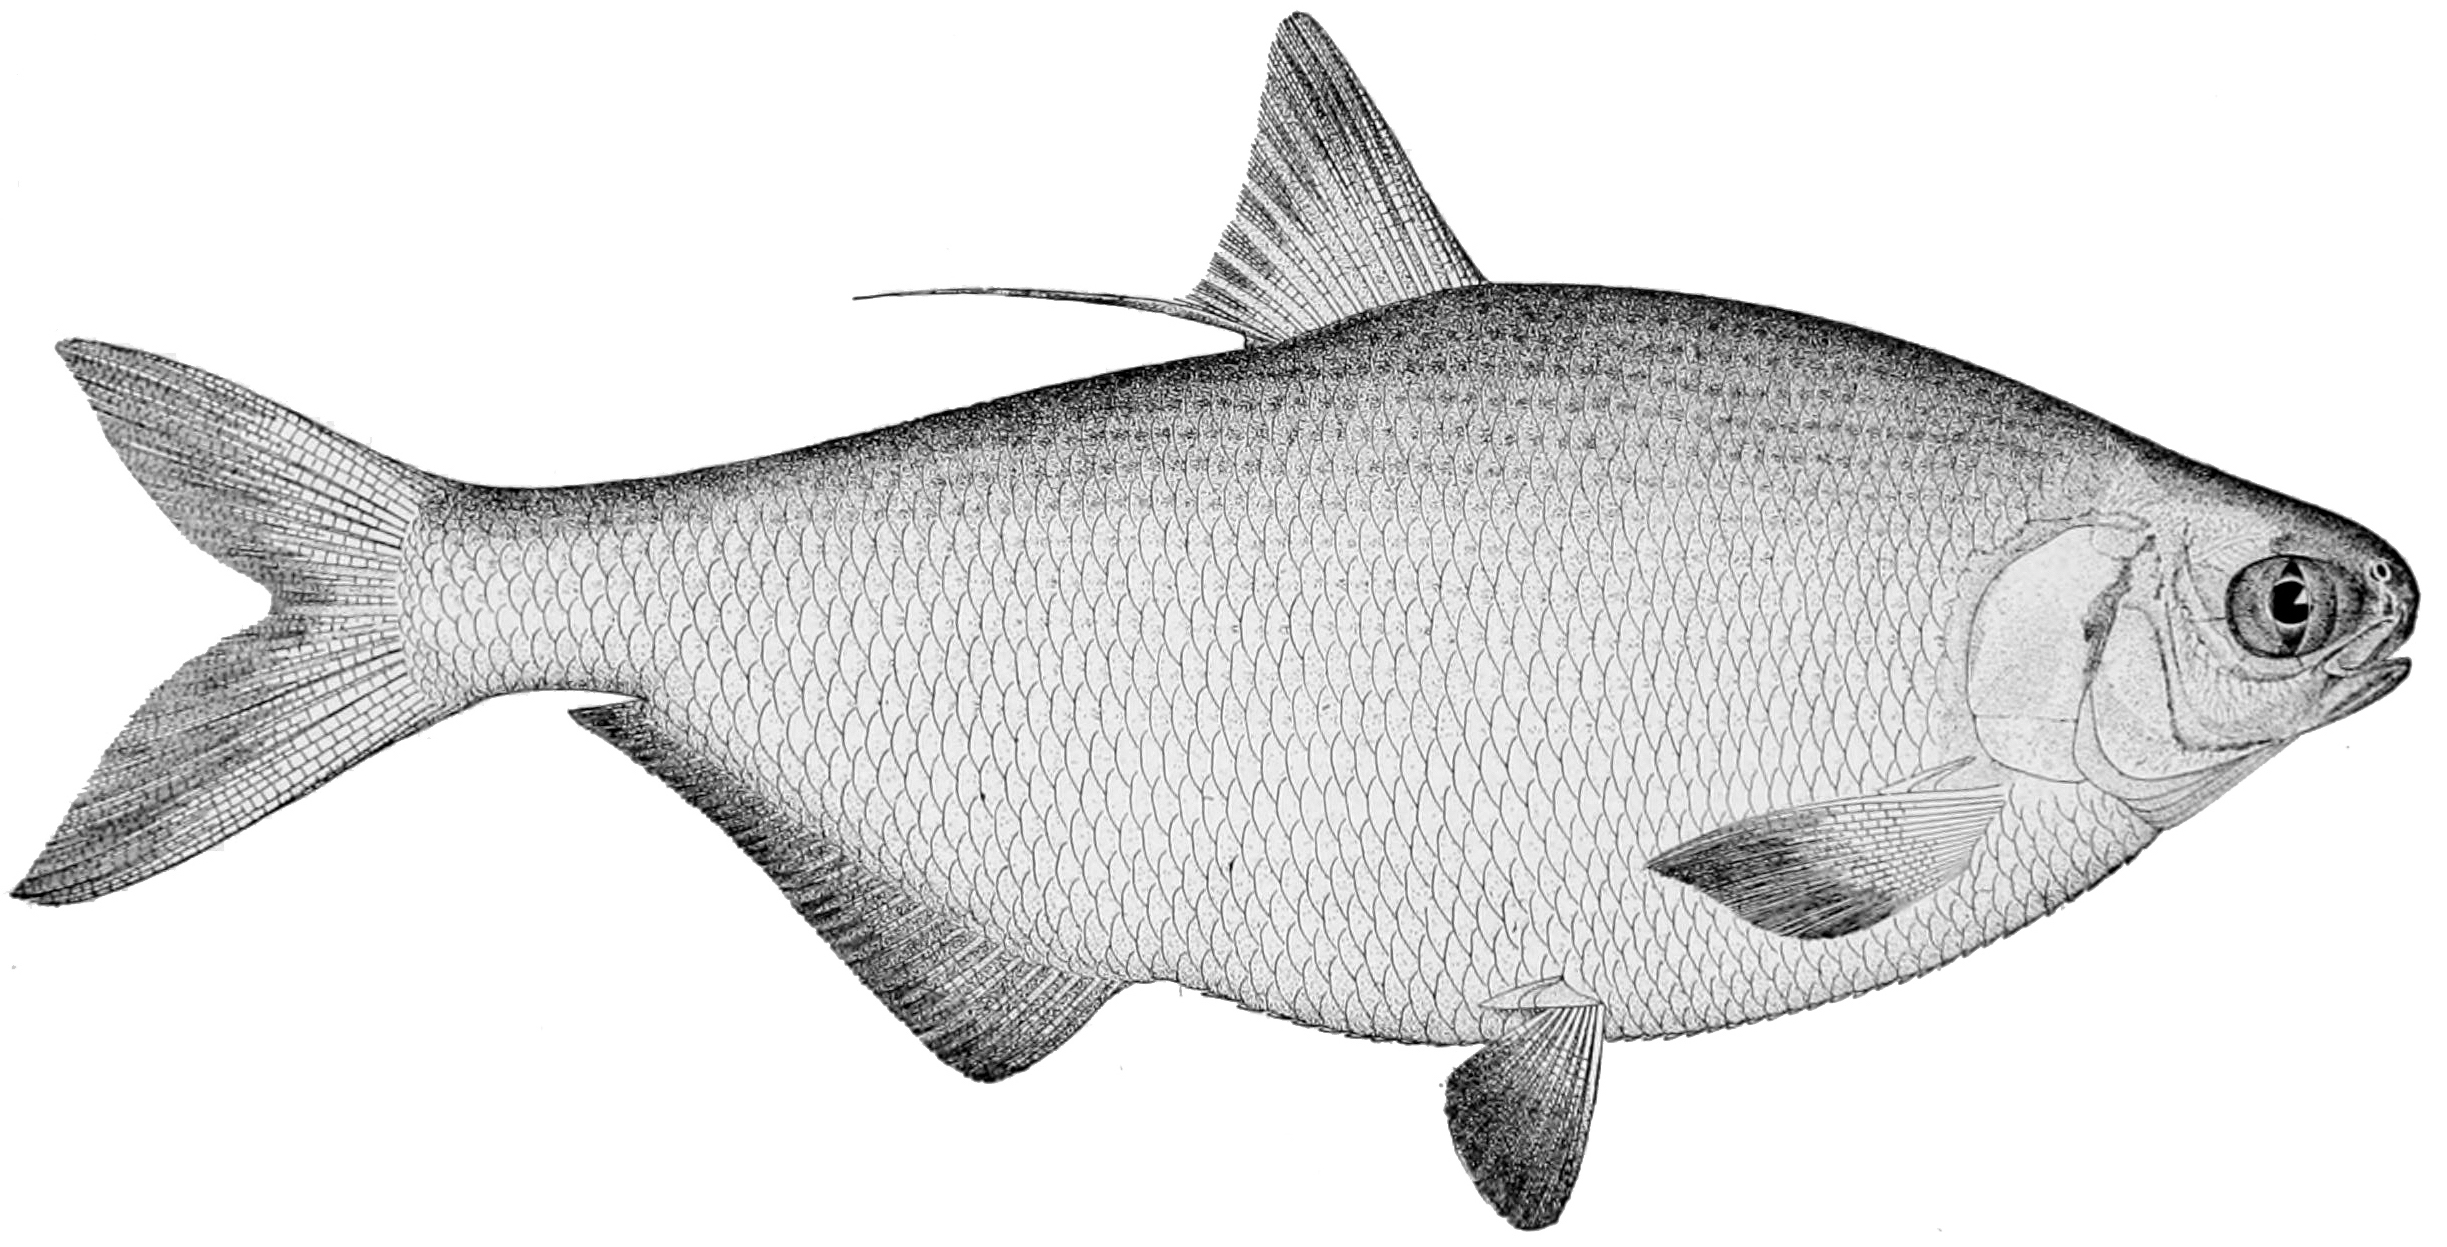
\includegraphics[width=0.15\textwidth]{adult.jpeg}\\
%        };
\node (grow_box) at (6.3,3.85) {Survival \& Growth};
\node[main node, align=center] (census_next) at (10,3) {Census $t+1$ \\
        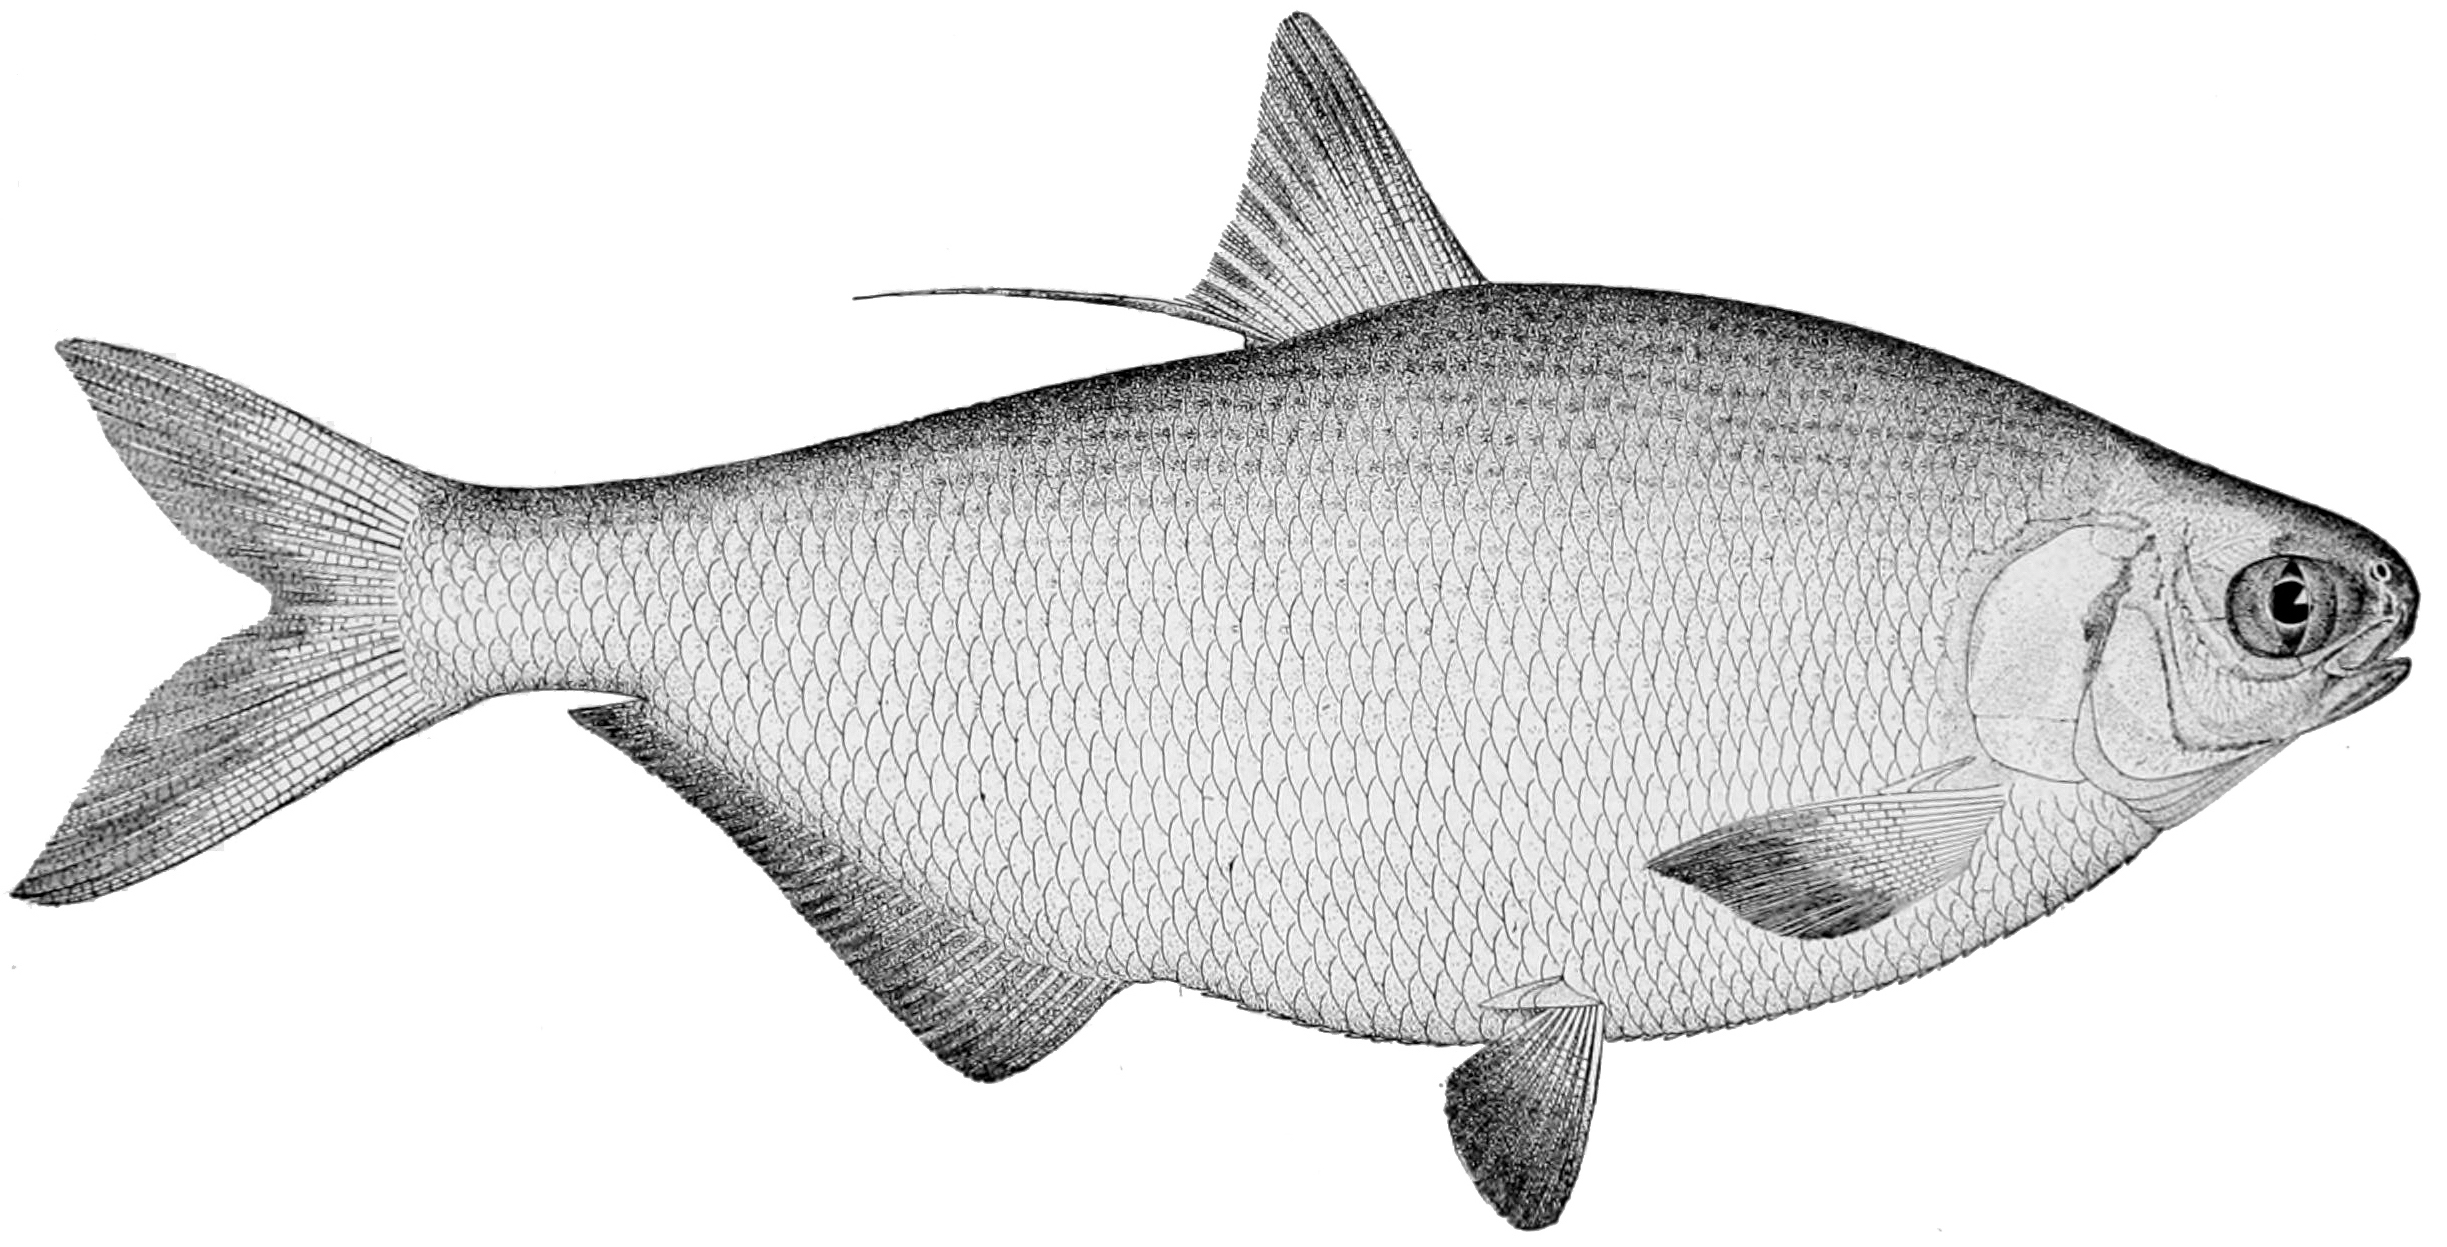
\includegraphics[width=0.15\textwidth]{adult.jpeg}\\
        $n(z',t+1)$};
\node (repro_box) at (13,3.85)  {Reproduction};
\node[align=center] (eggs) at (3,0) {Eggs \\ $\bullet$ $\bullet$ $\bullet$ $\bullet$ \\
  \, $\bullet$ $\bullet$ $\bullet$ $\bullet$ \\ $\bullet$ $\bullet$ $\bullet$ $\bullet$};
  \node[align=center] (eggs_viable) at (5,0) {Viable \\ $\bullet$ $\bullet$ $\bullet$ \\
  \, $\bullet$ $\bullet$ \\ $\bullet$ $\bullet$ $\bullet$};
 \node[align=center] (age1) at (8,0) { Age-1\\
        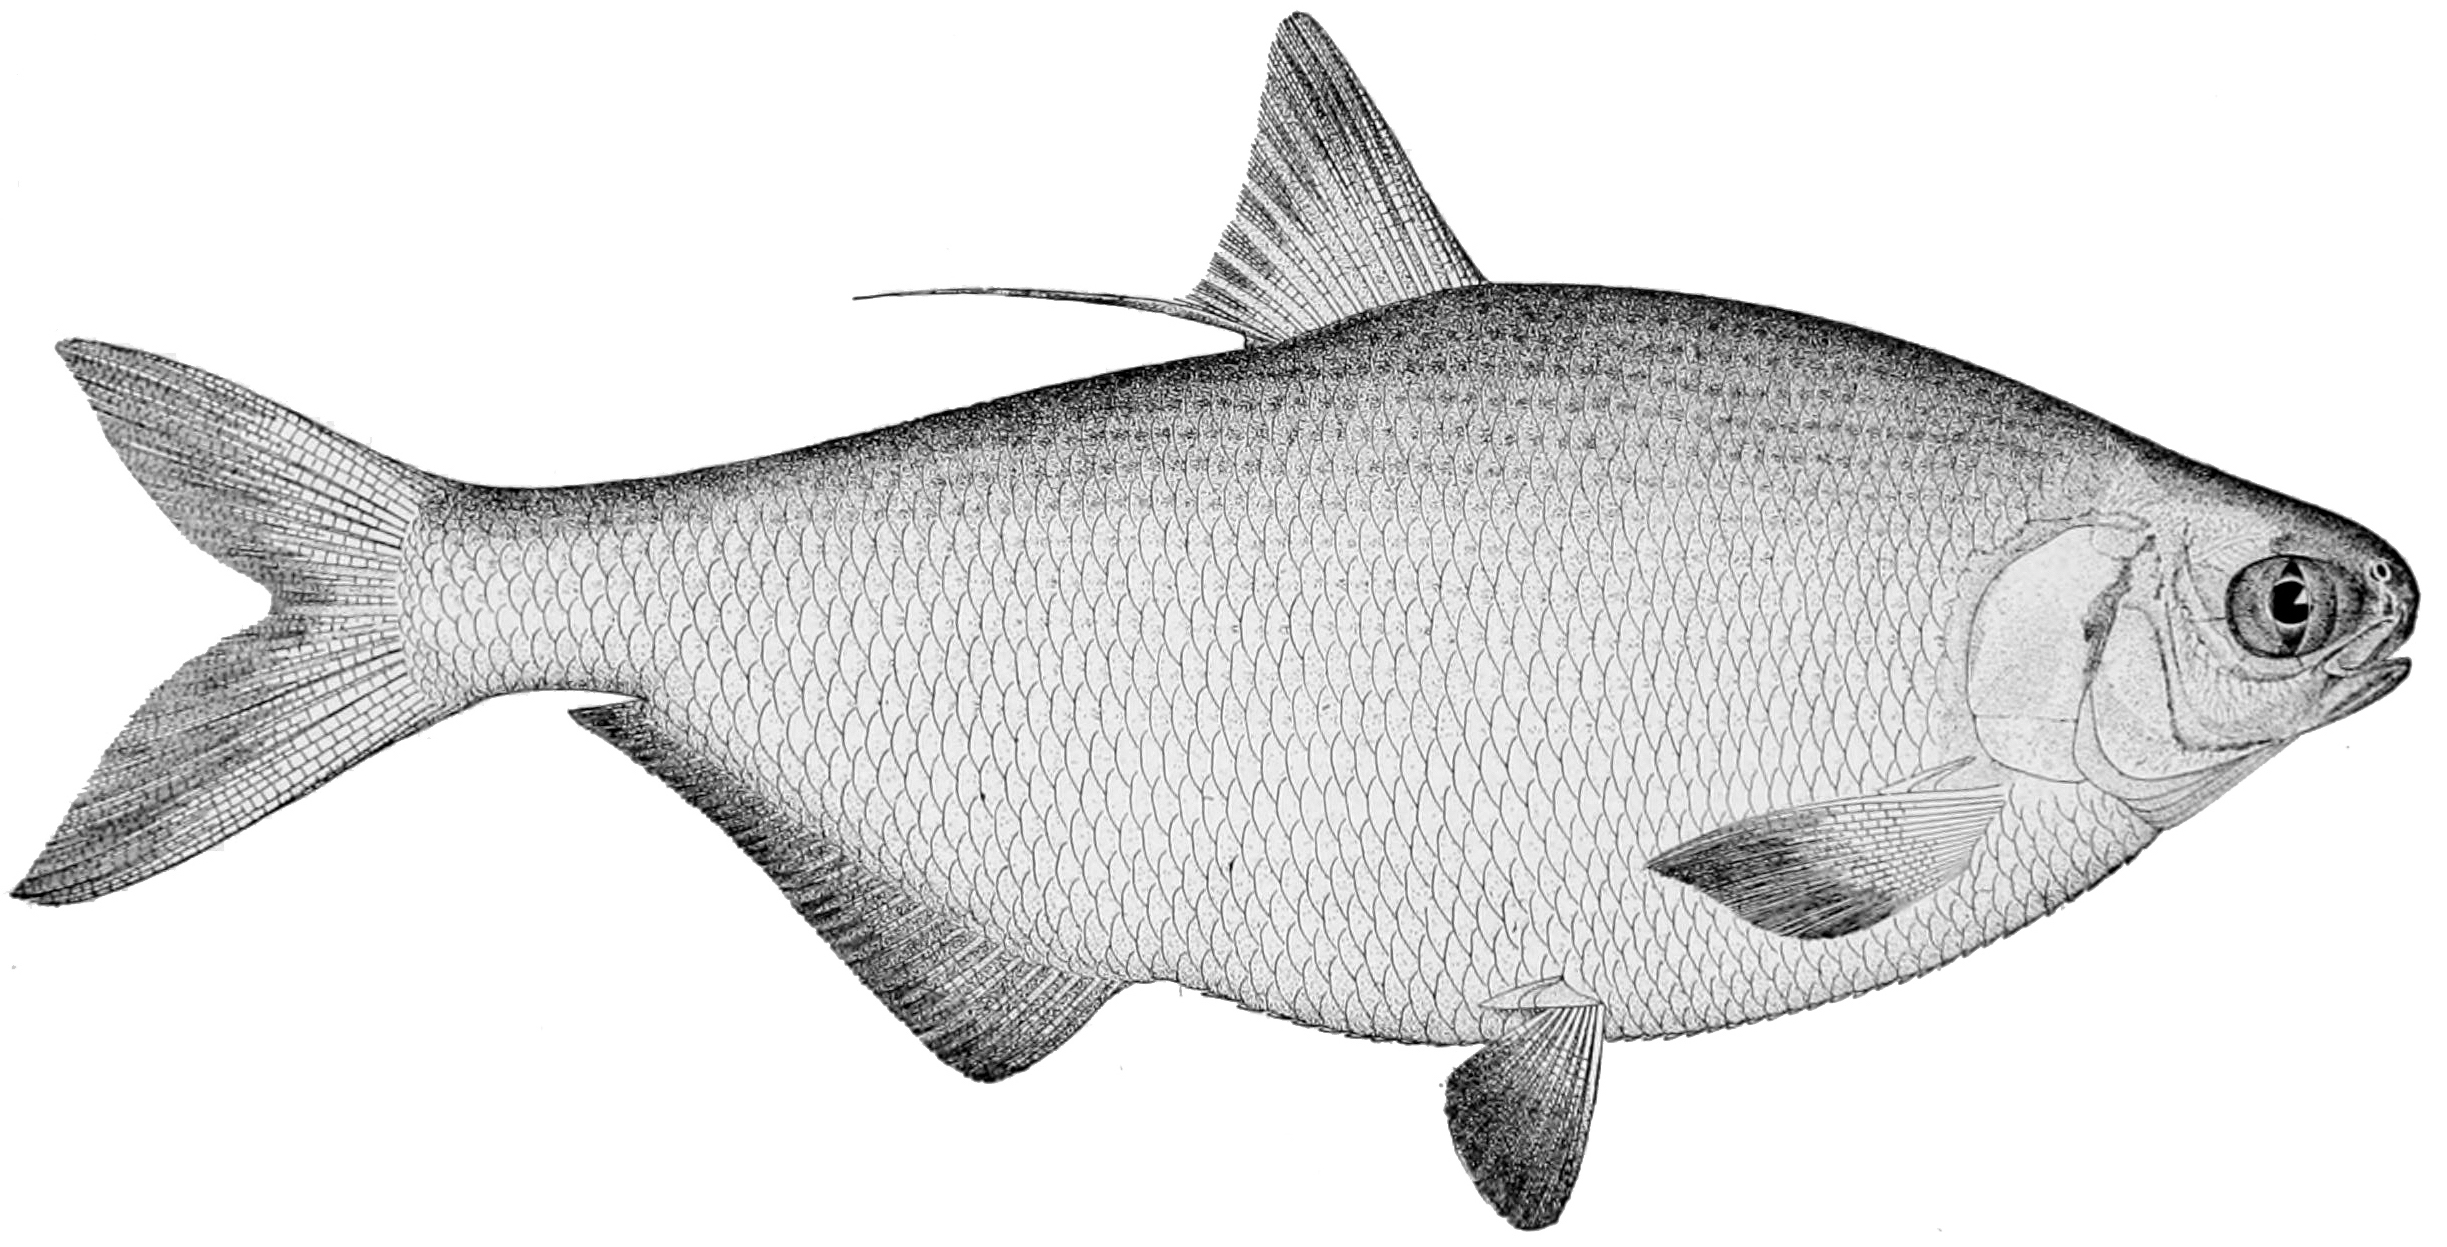
\includegraphics[width=0.06\textwidth]{adult.jpeg}
         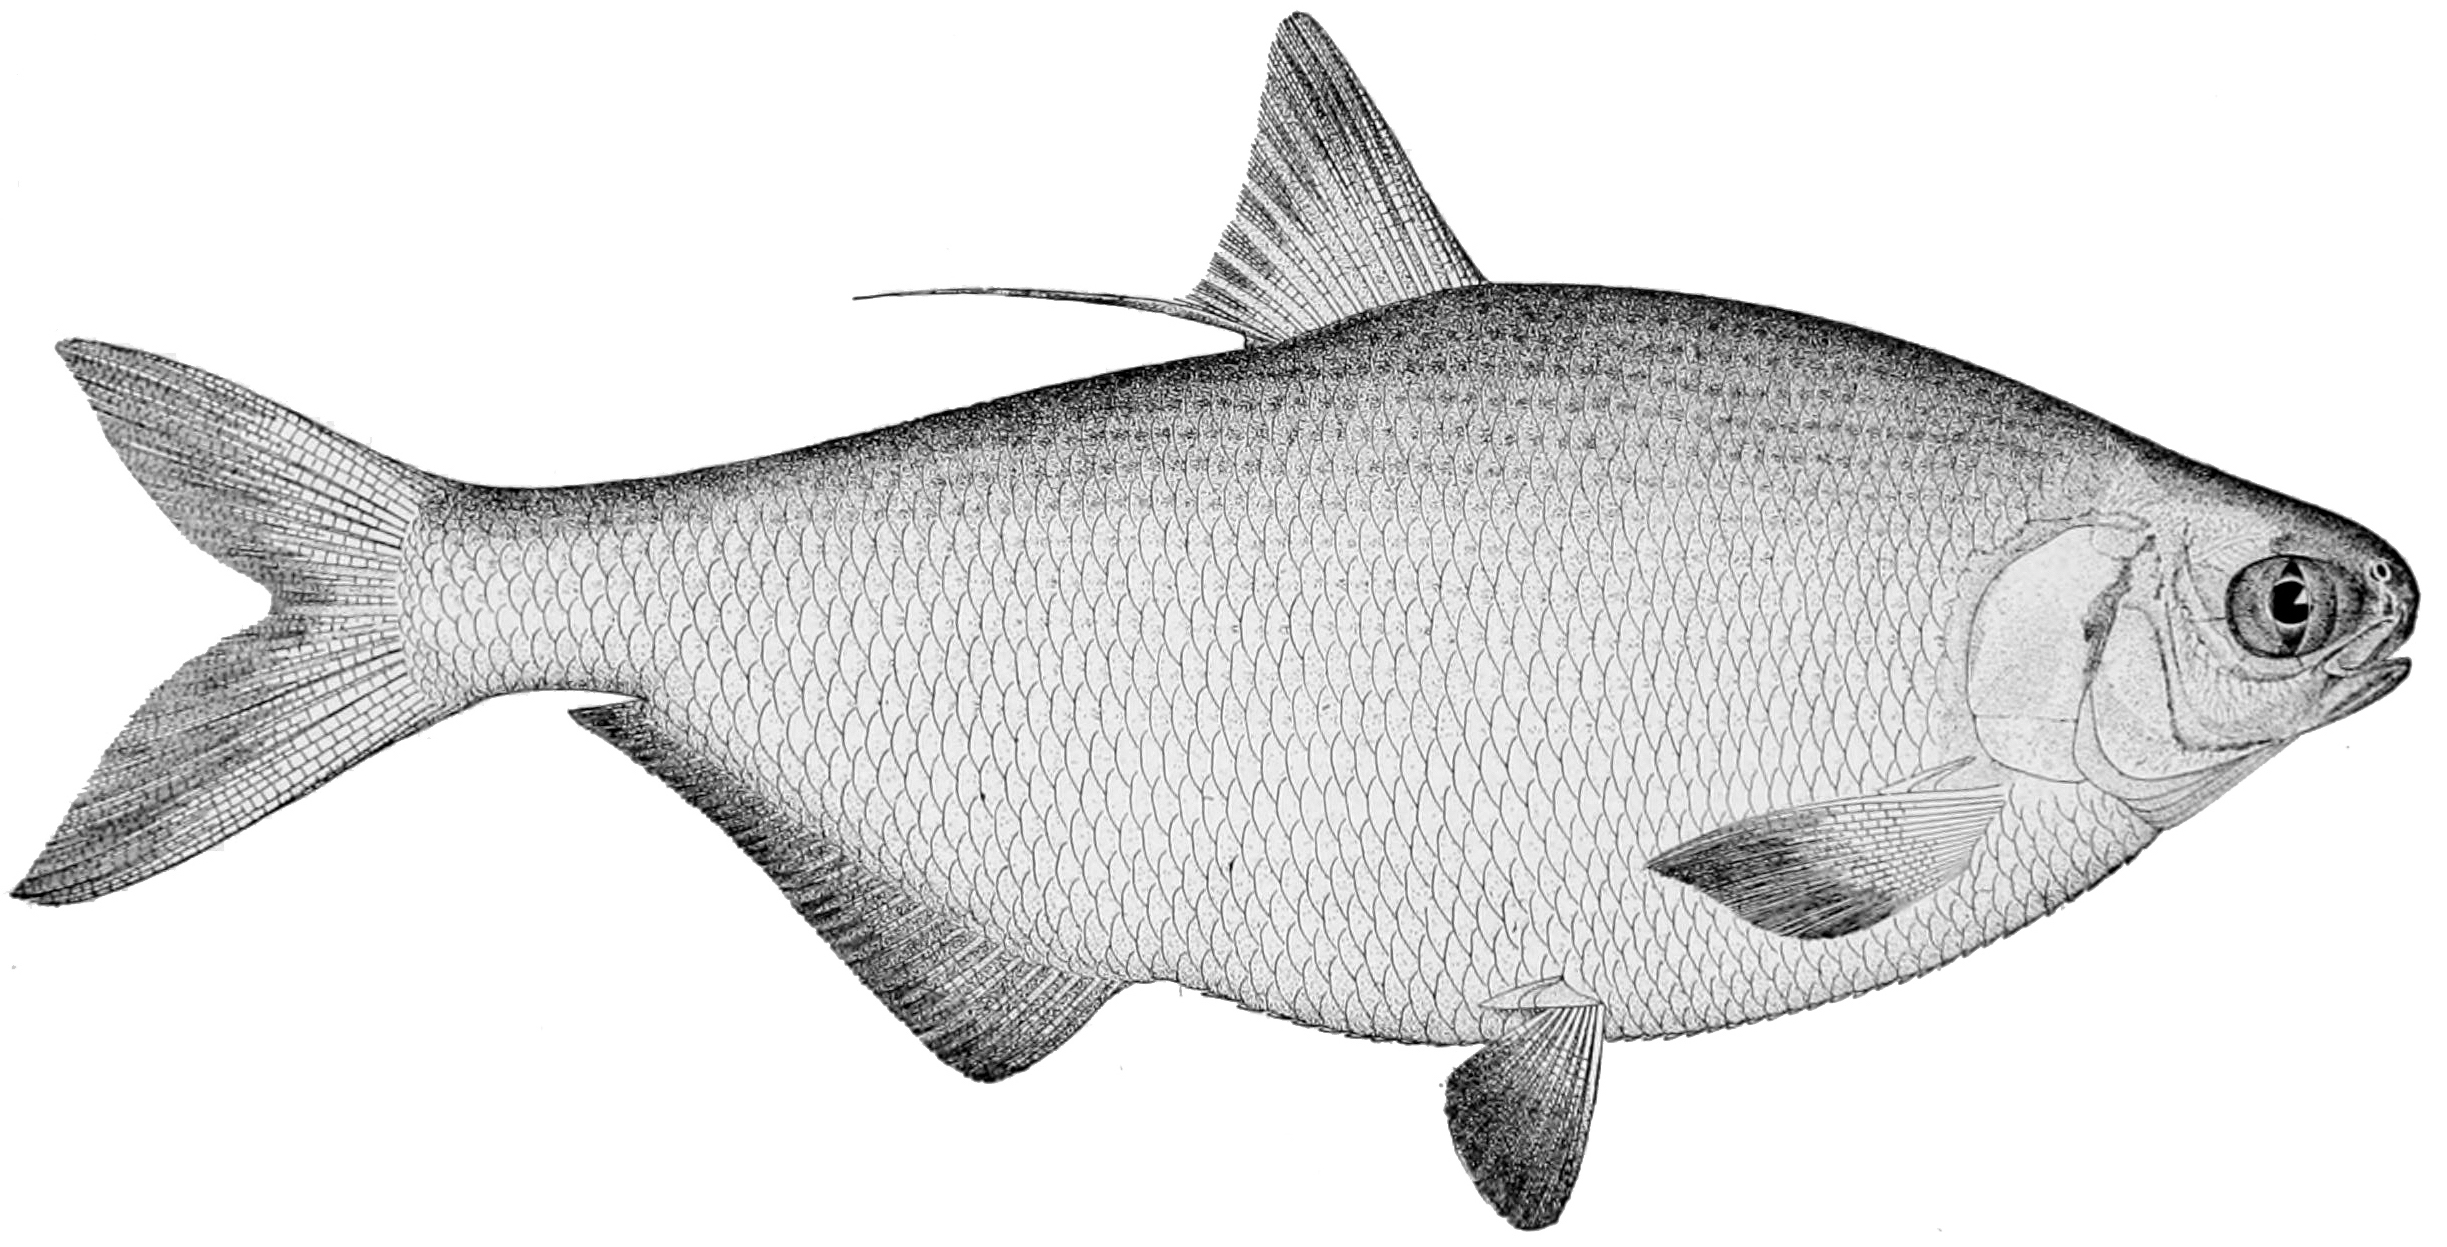
\includegraphics[width=0.04\textwidth]{adult.jpeg}\\
         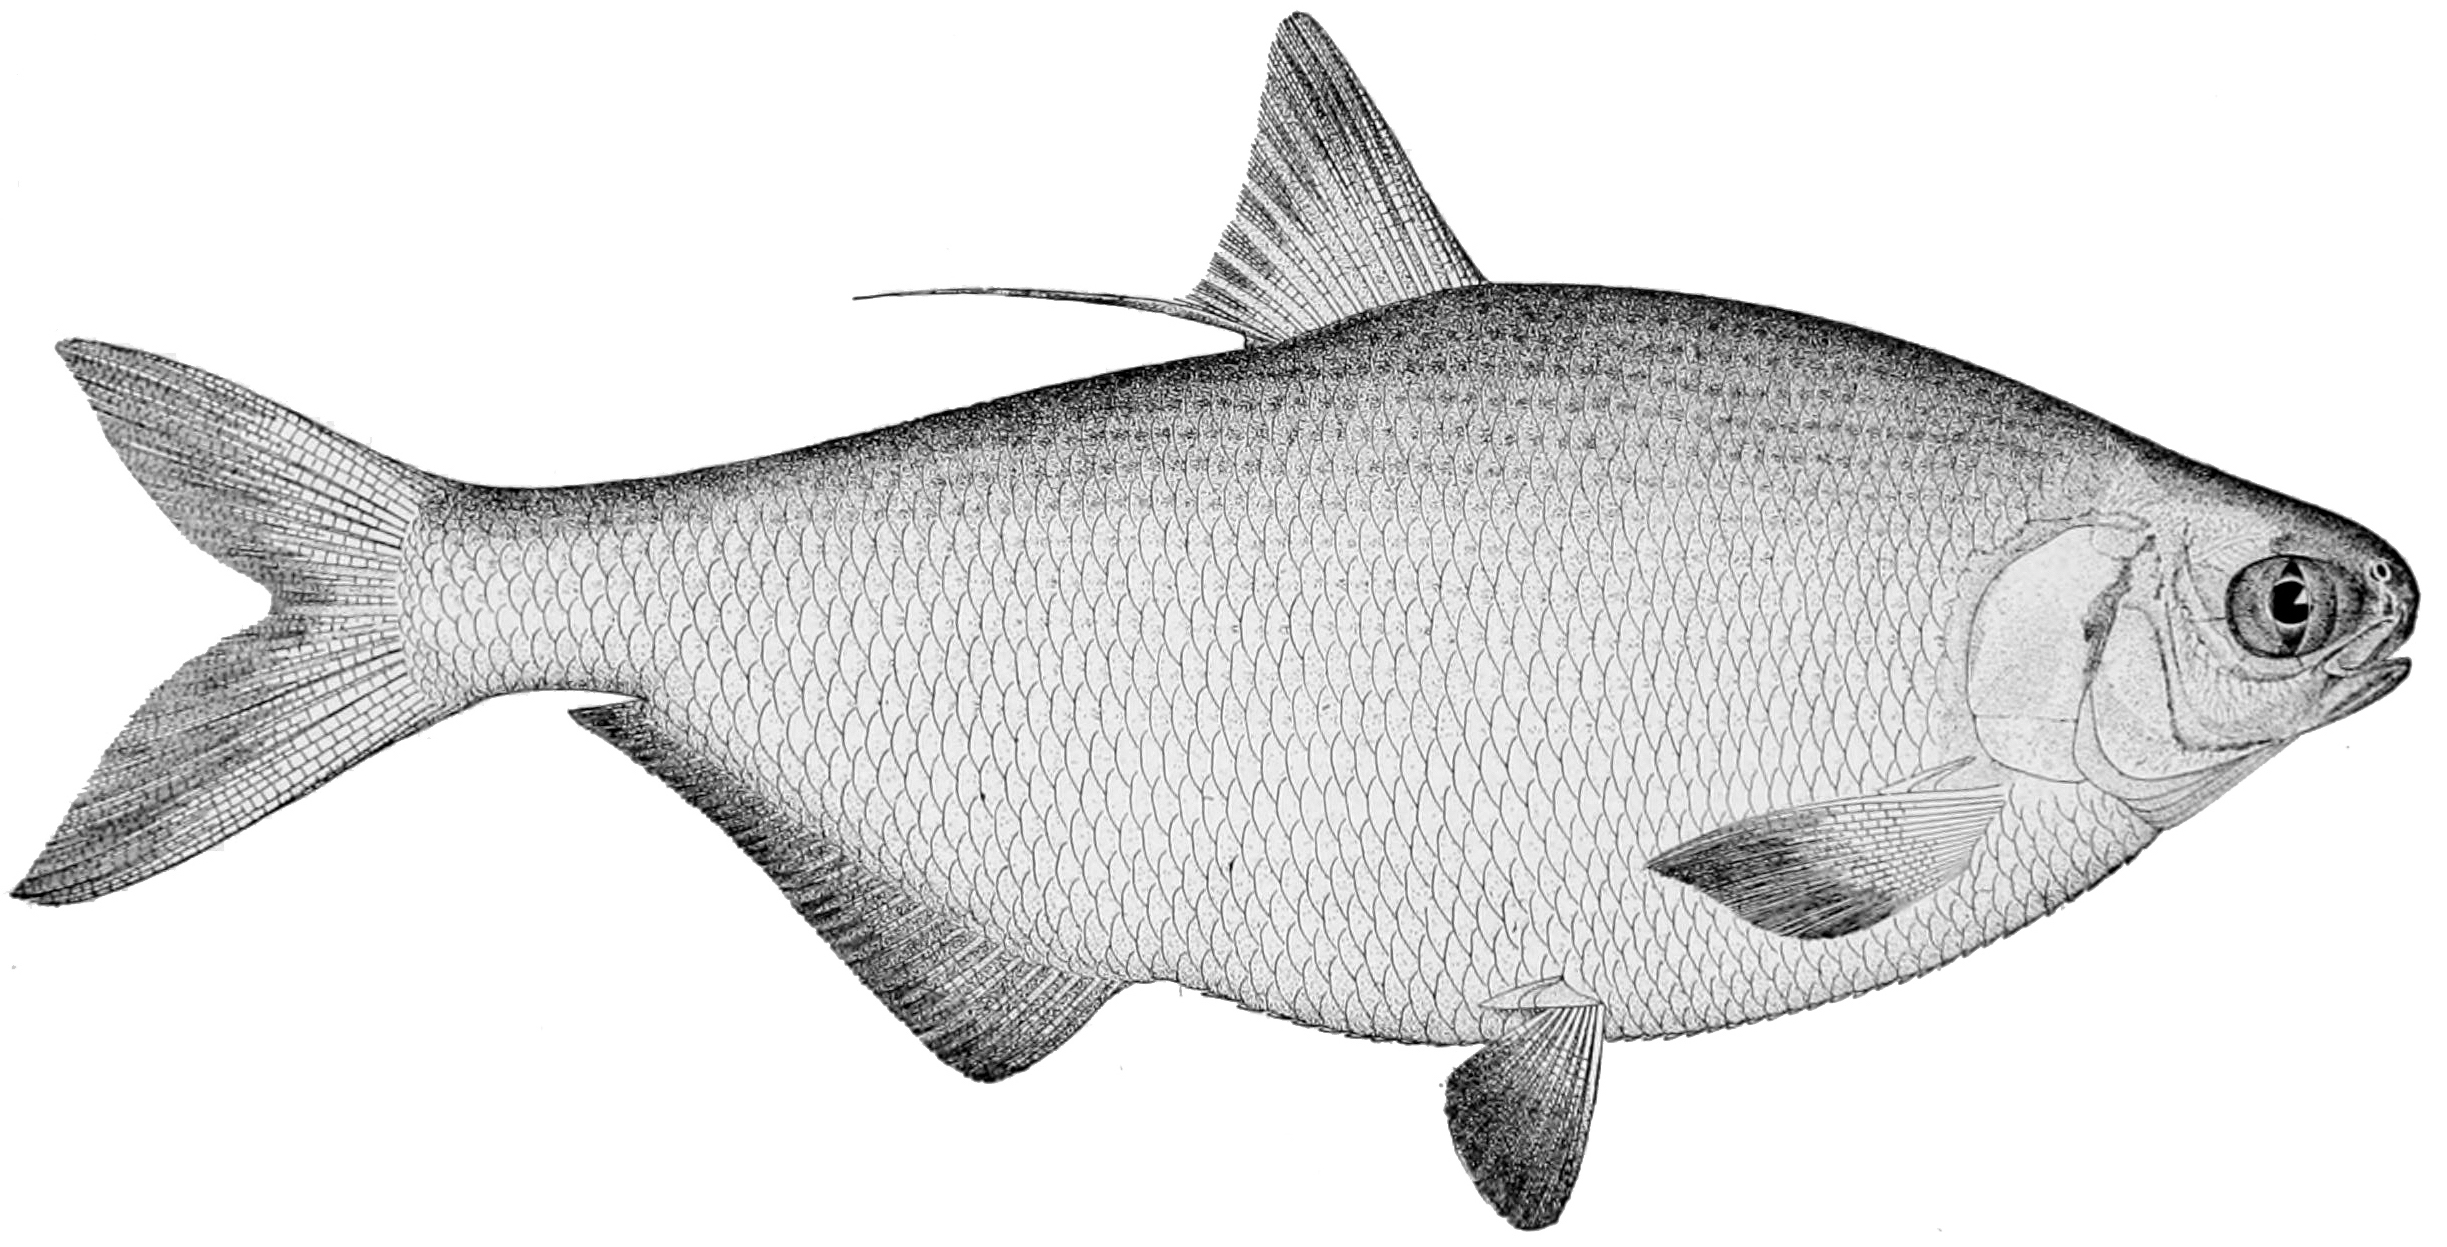
\includegraphics[width=0.08\textwidth]{adult.jpeg}
        };
\node[] (next) at (13,3) {};

\path[->]
	(census_pres) edge node {} (repro_in)
	(repro_out) edge node {$s(z)G(z',z)$} (census_next)
	(census_next) edge node {} (next)
	(repro_down) edge node {$p_b \rm{egg}(z)$} (eggs)
	(eggs) edge node {$\nu$} (eggs_viable)
	(eggs_viable) edge node {$s_0(d)$} (age1)
	(age1) edge node[right, pos=0.3] {$C_1(z')$} (census_next);
	
\end{tikzpicture}
%}
\end{center}
 \caption{\small{Life cycle diagram and census points for pre-reproduction census of gizzard shad.}}
\end{figure*}

\end{graphicalabstract}

%%Research highlights
\begin{highlights}
\item Research highlight 1
\item Research highlight 2
\end{highlights}

\begin{keyword}
  population dynamics \sep
  fisheries \sep
  Mississippi River basin \sep
  population ecology \sep
  invasive species impact 
%% keywords here, in the form: keyword \sep keyword

%% PACS codes here, in the form: \PACS code \sep code

%% MSC codes here, in the form: \MSC code \sep code
%% or \MSC[2008] code \sep code (2000 is the default)

\end{keyword}

\end{frontmatter}

%% \linenumbers

%% main text


\section{Introduction}
Gizzard shad (\emph{Dorosoma cepedianum}) is a laterally compressed, deep-bodied fish species that occupies numerous aquatic systems throughout central, southern and eastern regions of the United States \citep{pierce1981aspects,vanni2005linking}.  In more eutrophic habitats, such as reservoirs, gizzard shad can reach high abunadances and can come to dominate fish assemblages. Because of this, gizzard shad have the potential to influence freshwater systems in a number of ways. 
First, young shad often serve as a critical food source for many fish species, including those of commercial and recreational importance (such as walleye and largemouth bass)\citep{jester1972life}. Thus, this species can serve as an important trophic link within aquatic food webs.
Second, because detritus can serve as a primary food source throughout much of gizzard shad development (i.e. from the age-0 stage onward), these fish can transport nutrients
from benthic regions into pelagic habitats \citep{mather1995regeneration, schaus2000effects, vanni2005linking}. 
This process can result in an increase in the nutrients available to organisms within the water column leading to increases in phytoplankton biomass, algal blooms, and, due to these conditions, shifts in freshwater community structure \citep{aday2003direct, schaus2000effects}. 
Finally, the fact that detritus can comprise a substantial portion of gizzard shad diet also makes this species an important connector between terrestrial inputs and aquatic processes \citep{schaus2000effects}.
Given its potentially important role in aquatic ecosystems, interest has intensified in understanding how gizzard shad populations respond to environmental changes (both natural and anthropogenic) and what these changes may mean for freshwater communities in general and fish assemblages in particular.

Interactions within and between species in interconnected environments can have important consequences for fish populations across space and time \citep{thorp2006riverine}.  For gizzard shad, previous work has suggested that fish densities can play an important role in the length-distribution patterns observed in populations.  For example, Buynak et al. (1992) and Welker et al. (1994) reported inverse relationships between densities and lengths in age-0 gizzard shad under both field and semi-natural conditions.  These patterns were attributed to intraspecific competition among young shad for prey (zooplankton) resources. Although intraspecific competition may be occurring in subsequent stages of gizzard shad development, little work has actually been conducted to address this (Dicenzo et al., 1996). There is also evidence that the densities of other co-occurring fish species (such as invasive carps) can negatively influence aspects of gizzard shad biology, such as body condition (Irons et al. 2007, Love et al. 2018).     

%[NEED] Paragraph about density effect on fish species in Upper
%Mississippi River.
%While present density of gizzard shad may influence the growth and
%survival of adults, we emphasize our present investigation the role
%density has in age-0 survival.


Although substantial empirical work on gizzard shad biology has accumulated over the decades, few if any studies have attempted to use these data to model the population dynamics of the gizzard shad.
Work by \citet{catalano2010size, catalano2011whole} used empirically-based simulations of gizzard shad and focused on population-level responses.
This work did examine population-structure by examining length and did
not explore different sources of density feedback on the population
dynamics.
Here, we introduce an integral projection model for gizzard shad based on empirical data with density-dependent survival in age-0 fish.
We then compare model outcomes to dynamics reported for this fish species in the La Grange Station along the Illinois River.
The model itself could be an important tool for predicting gizzard shad population responses to changing environmental conditions, including those mediated through species invasions (i.e., silver and bighead carp).

\begin{table*}
  \caption{A summary of parameters, their biological meaning, and source for mean values.
  }
 \begin{center}
	\resizebox{\textwidth}{!}{
\begin{tabular}{p{6.5cm}|p{6cm}|c| p{6cm}  }\hline
     Parameter & Meaning (units) & Mean& Source \\\hline
Logistic survival probability function, $s(z)$ & & \\
  $\ds s_{\rm {min}}$ & minimum survival & 0.002 & \citep{bodola1955life} \\
  $\ds s_{\rm {max}}$ & maximum survival & $\ds 1-8.871K^{0.73}L_{\infty}^{-0.33}$ 
  & THEN 2015 \\ 
 $\ds \alpha_s$  & inflection point & 103.53 & modeled from LTRM dataset \\
  $\ds \beta_s$ & slope & -943.89 & modeled from LTRM dataset \\\hline
  Growth function, $\ds G(z,z')$ & & \\
  $L_\infty$ & maximum length (in mm) & 394.30 & \citep{catalano2010size} \\
  $K_g$ & growth rate & 0.26 &  \citep{michaletz2017variation} \\
  $\sigma_g$ & growth standard deviation & 25 &  \citep{michaletz2017variation} \\\hline
  Normal distribution of length of age-1, $\ds C_1(z')$ & & \\
  $\mu_r$ & mean length of recruitment (in mm) & 105 & \citep{michaletz2017variation} \\
  $\sigma_r$  & standard deviation of length & 25 & \citep{michaletz2017variation} \\\hline
Eggs produced, egg(z) & & \\
$\ds \mbox{egg}_{\mbox{max}}$ & maximum number of eggs produced & 742,094 & Estimated from \citep{jons1997ovarian} \\
$\ds \alpha_e$ & inflection point & 314.44 & Estimated from \citep{jons1997ovarian} \\
$\ds \beta_e$ & slope & -7.12 & Estimated from \citep{jons1997ovarian} \\\hline
Survival of age-0, $s_0(d(t))$ & & \\
$\ds a_0$ & intercept & 0.27 & Estimated from \citep{michaletz2010overwinter} \\
$\ds b_0$ & decay rate & 0.003 & Estimated from \citep{michaletz2010overwinter} \\\hline
Spawning & & \\ 
 $\nu$  & probability that egg becomes viable & 0.002 & \citep{bodola1955life} \\
 $p_b$ & probability that female spawns & 0.90 &    \\ 
 \end{tabular} } \label{table:parameters}
     \end{center}
     \end{table*}    

\section{Model Development}
\subsection{Gizzard shad life history}
Mating within this species can be temperature-dependent, but tends to occur between May and June. 
Males and females aggregate and then broadcast gametes into the surrounding water; fertilized eggs then settle and adhere to the bottom substrates. 
After a period of days, eggs hatch and fish develop from the larval stage to juveniles and eventually to adults. 
In many habitats, individuals can reach sexual maturity within a year. As gizzard shad mature, their diet preferences typically shift from phytoplankton and zooplankton early in development to detritus and zooplankton as adults. 
Given the large number of eggs produced by shad females ($>$ 300,000/year), there is evidence that intraspecific competition can be intense during early developmental stages in this species. 
However, the strength of competition can subside as fish transition to different food types during latter stages of development.   

\subsection{Equations}
We used an integral projection model to describe the life history of gizzard shad in the Upper Mississippi River (UMR) system. 
Integral projection model (IPM) were introduced by Easterling \citep{easterling2000size}, as a generalization of stage-based, matrix population models. 
IPMs have been used to describe a wide range of organisms \citep{ellner2016data, merow2014advancing, rees2014building} and are a natural choice for gizzard shad since many aspects of their life cycle have been studied. 
Specifically, functions used in our model incorporate data from studies on egg production and adult size as well as the survival of the age-0 stage and density. 

We assumed that variations among individual gizzard shad can be summarized by its length $z$ (in mm) ranging from the minimum possible length $L$ to the maximum value $U$. 
The state of the population at time $t$ (in years) is described by the length distribution $n(z,t)$. 
Specifically, for each time $t$, $n(z,t)$ is a smooth function of $z$ such that the number of individuals of length $z$ in the interval $[a,b]$ at time $t$ is $\ds \int_a^b n(z,t) \, dz$. 

Between times $t$ and $t+1$, individual gizzard shad may grow, die, and produce offspring that vary in length depending on the individuals current length (Figure \ref{life_cycle}). 
At time $t+1$ the population will have a length distribution defined by $n(z, t+1)$. 
For our model, we partition the life cycle of gizzard shad into two stages: 1) survival and growth, and  2) reproduction. 
For an individual of length $z$ at time $t$, $P(z',z)\Delta z$ is the probability that the individual is alive at time $t+1$, and its size is in the interval $[z', z' + \Delta z]$ (as with $n(z,t)$ this is an approximation that is valid for small $\Delta z$, and the exact probability is given by an integral like the one above). 
Similarly. $F(z',z)\Delta z$ is the number of new offspring in the interval $[z', z' + \Delta z]$ present at time $t+1$, per length-$z$ individual at time $t$.

\begin{figure*}
\label{llife_cycle}
    \begin{center}
%\scalebox{.75}[.75]{
\begin{tikzpicture}[->,>=stealth',shorten >=1pt,auto,node distance=3cm,
  thick,
  main node/.style={rectangle,draw},
  box/.style = {draw=gray, very thick,
                            minimum height=11mm, text width=11mm, 
                            align=center},]
                              
\node[main node, align=center] (census_pres) at (0,3) {Census $t$ \\
        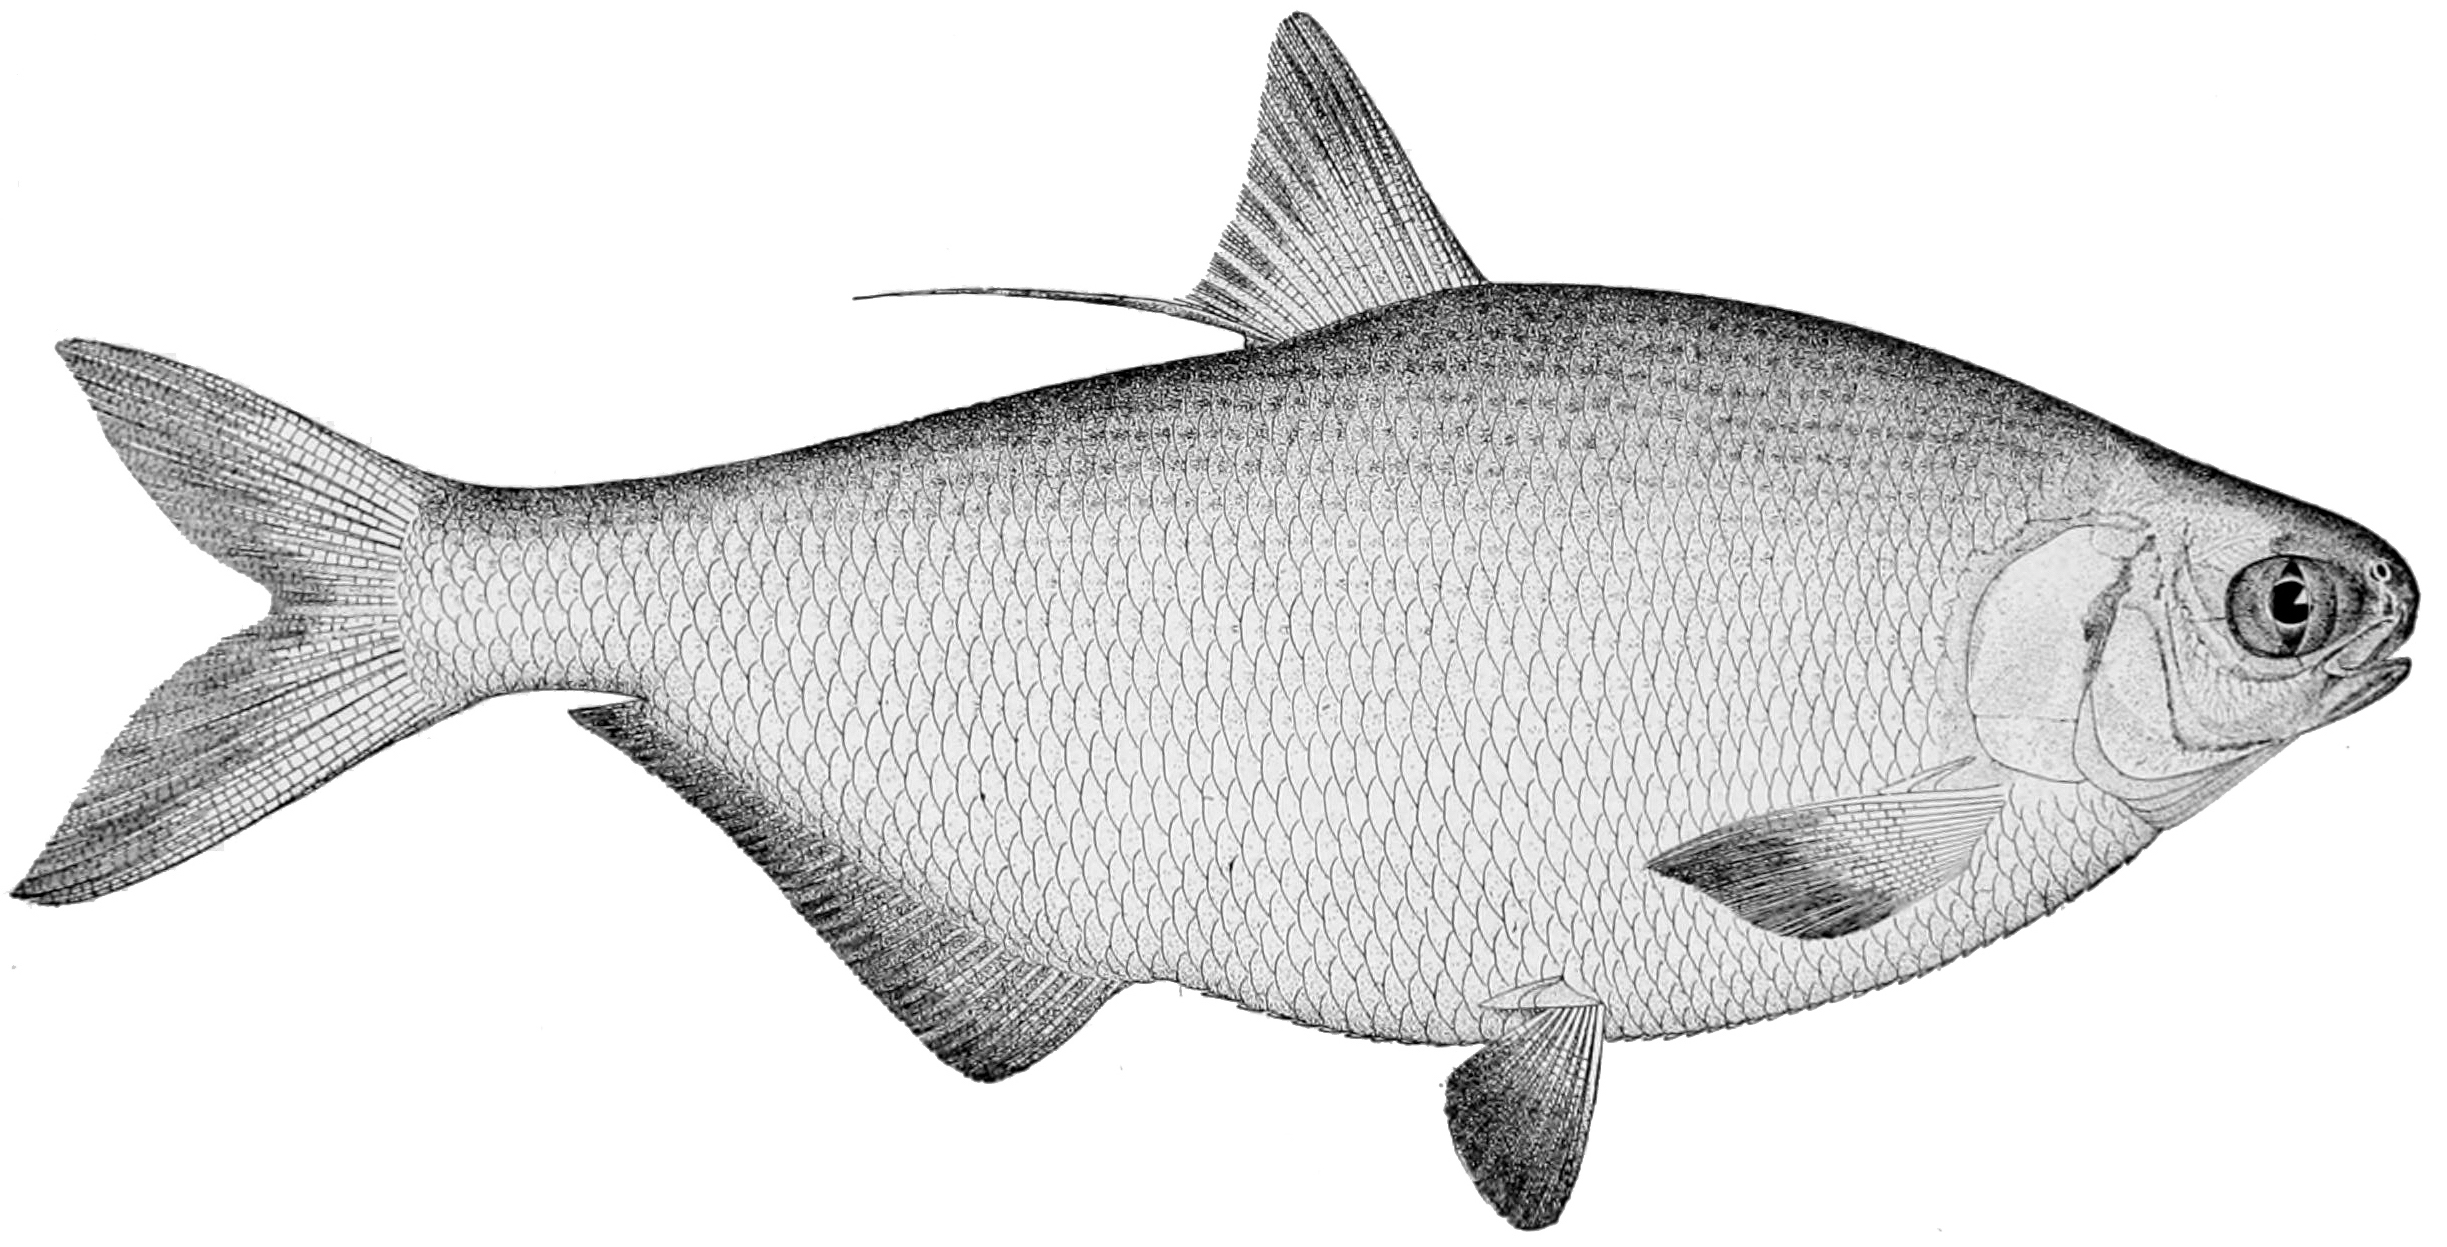
\includegraphics[width=0.12\textwidth]{adult.jpeg} \\
        $n(z,t)$};
\node[align=center] (repro) at (3.25,3) {Reproduction\\
        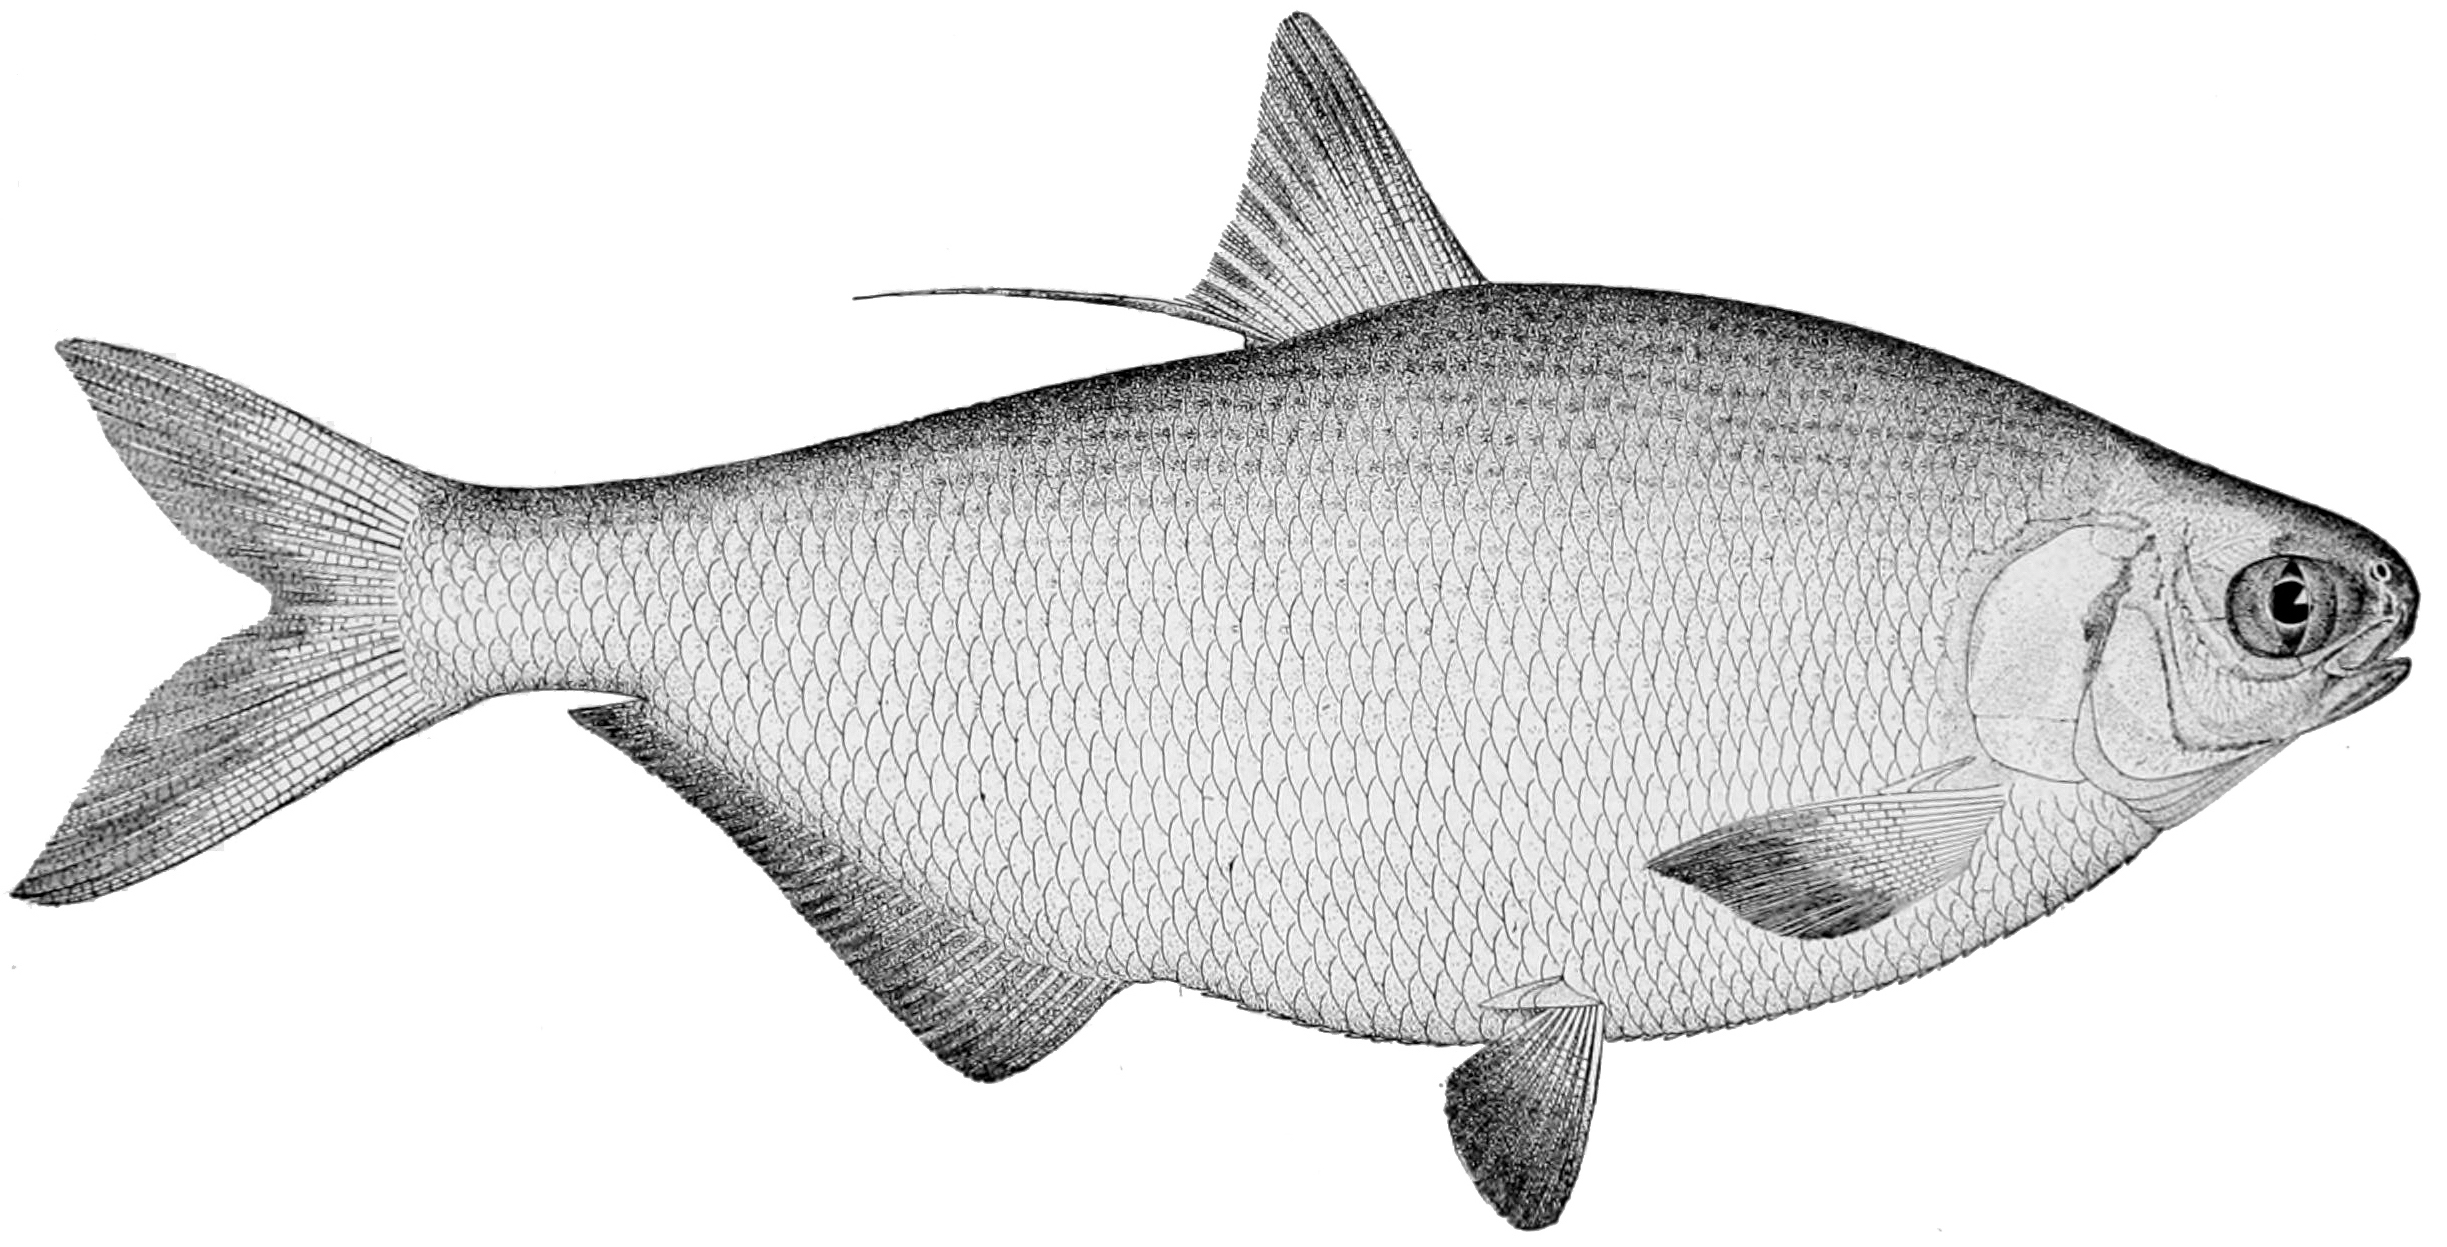
\includegraphics[width=0.12\textwidth]{adult.jpeg}\\
        };
\node (repro_in) at (2.3, 3)  {};
\node (repro_out) at (4.25, 3)  {};
\node (repro_down) at (3, 2.5)  {};
%\node[align=center] (surv) at (4.5,3) {\\
%        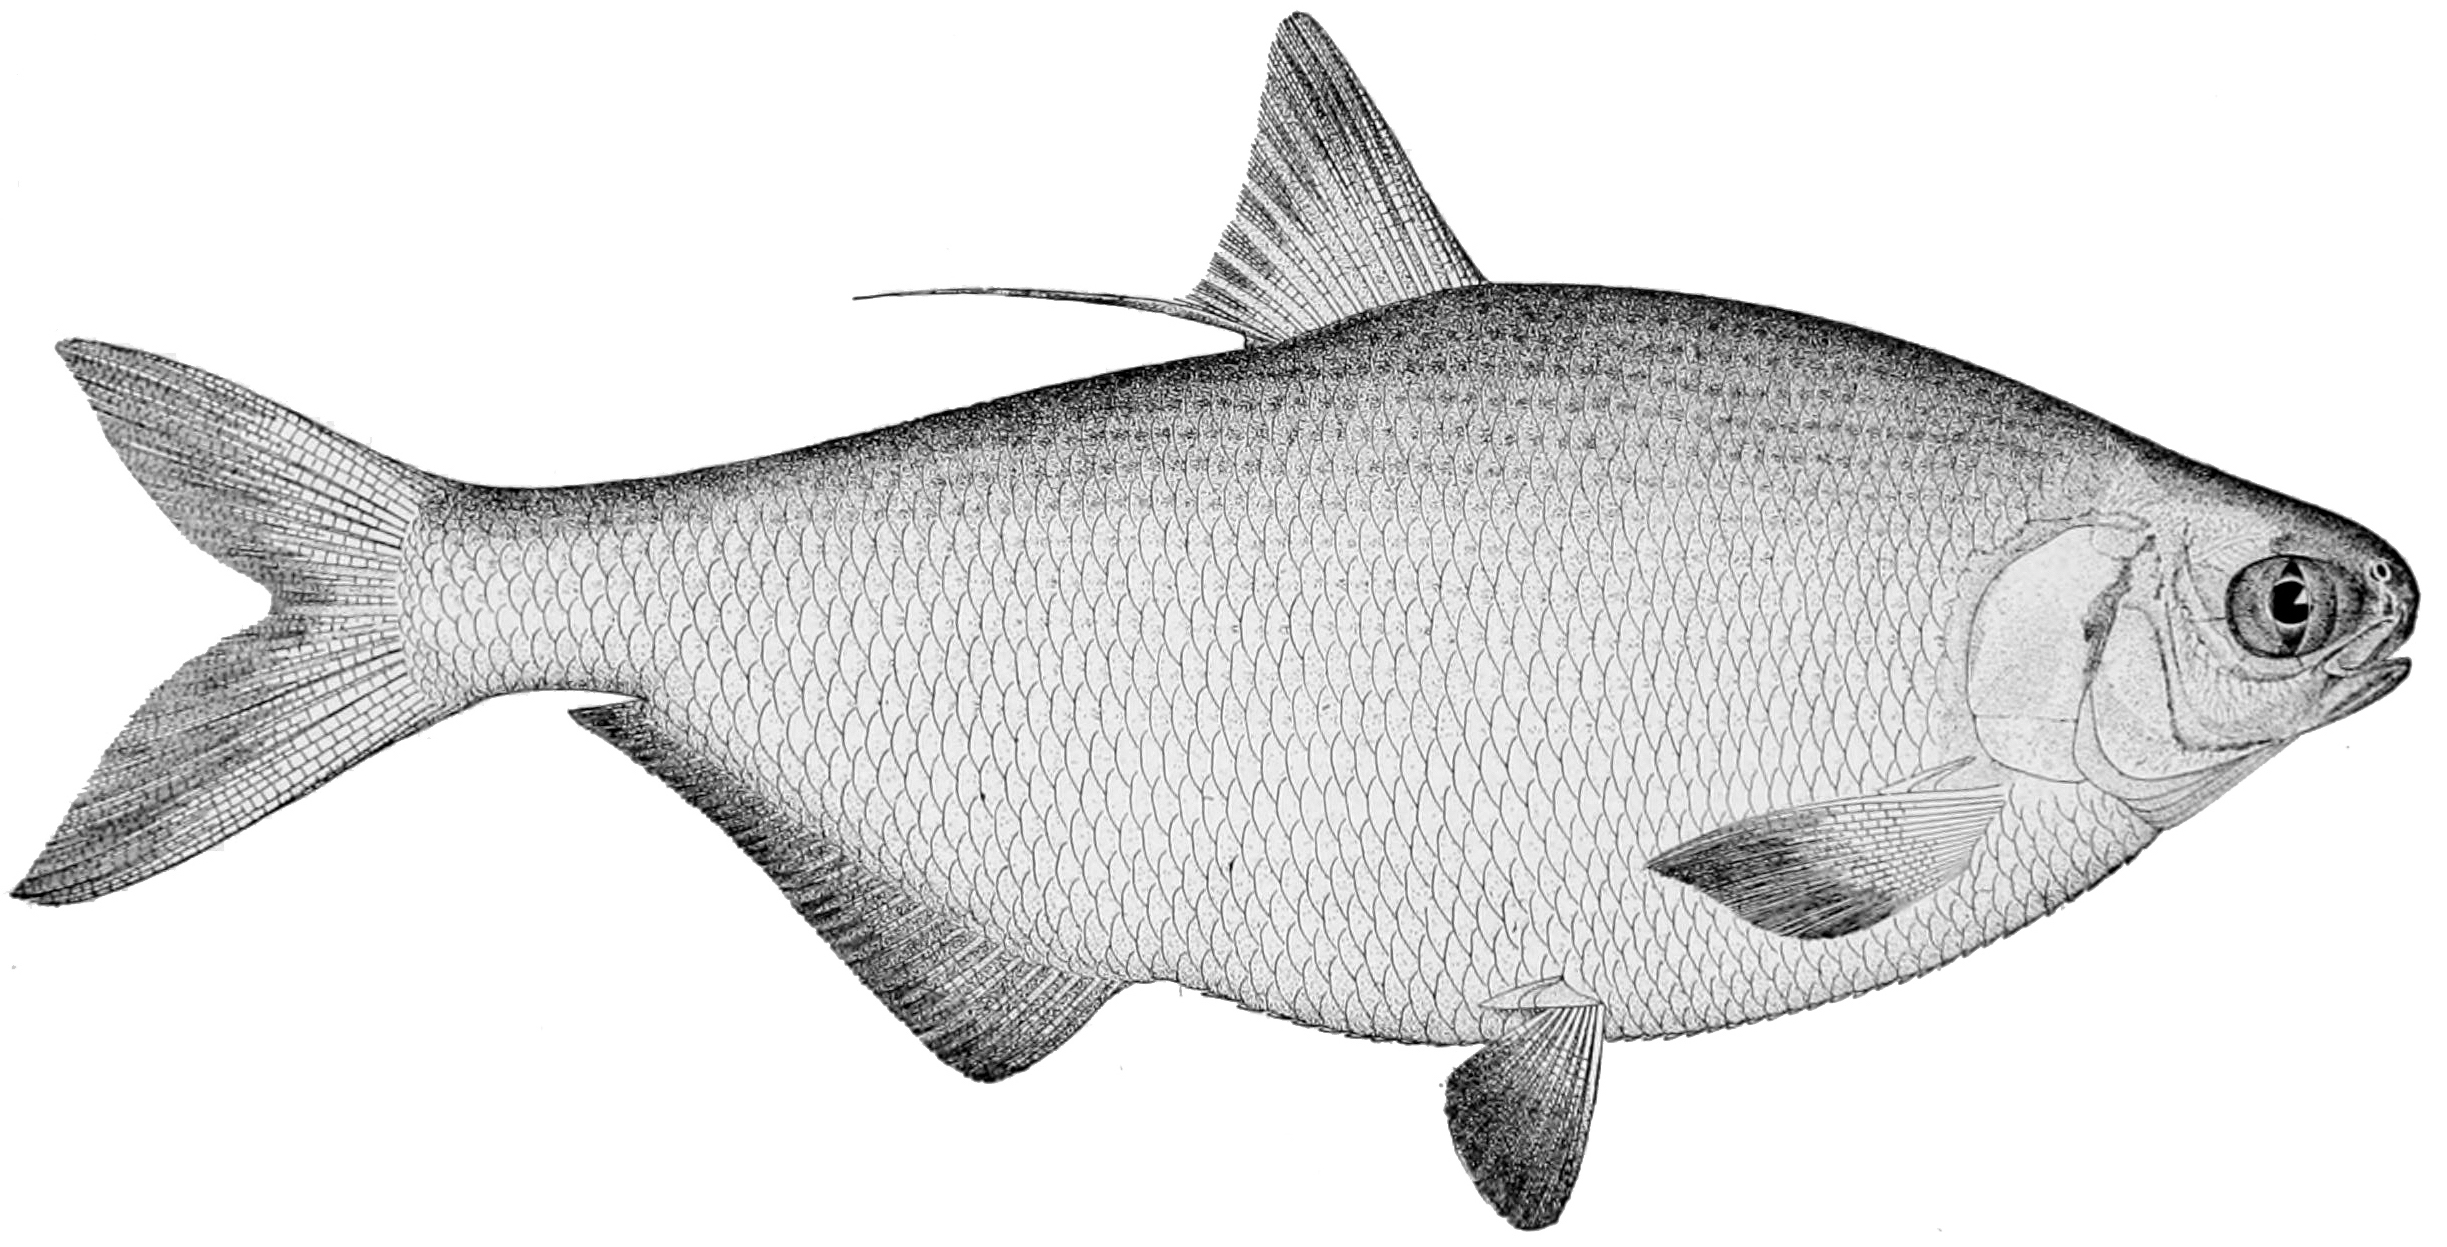
\includegraphics[width=0.15\textwidth]{adult.jpeg}\\
%        };
\node (grow_box) at (6.3,3.85) {Survival \& Growth};
\node[main node, align=center] (census_next) at (10,3) {Census $t+1$ \\
        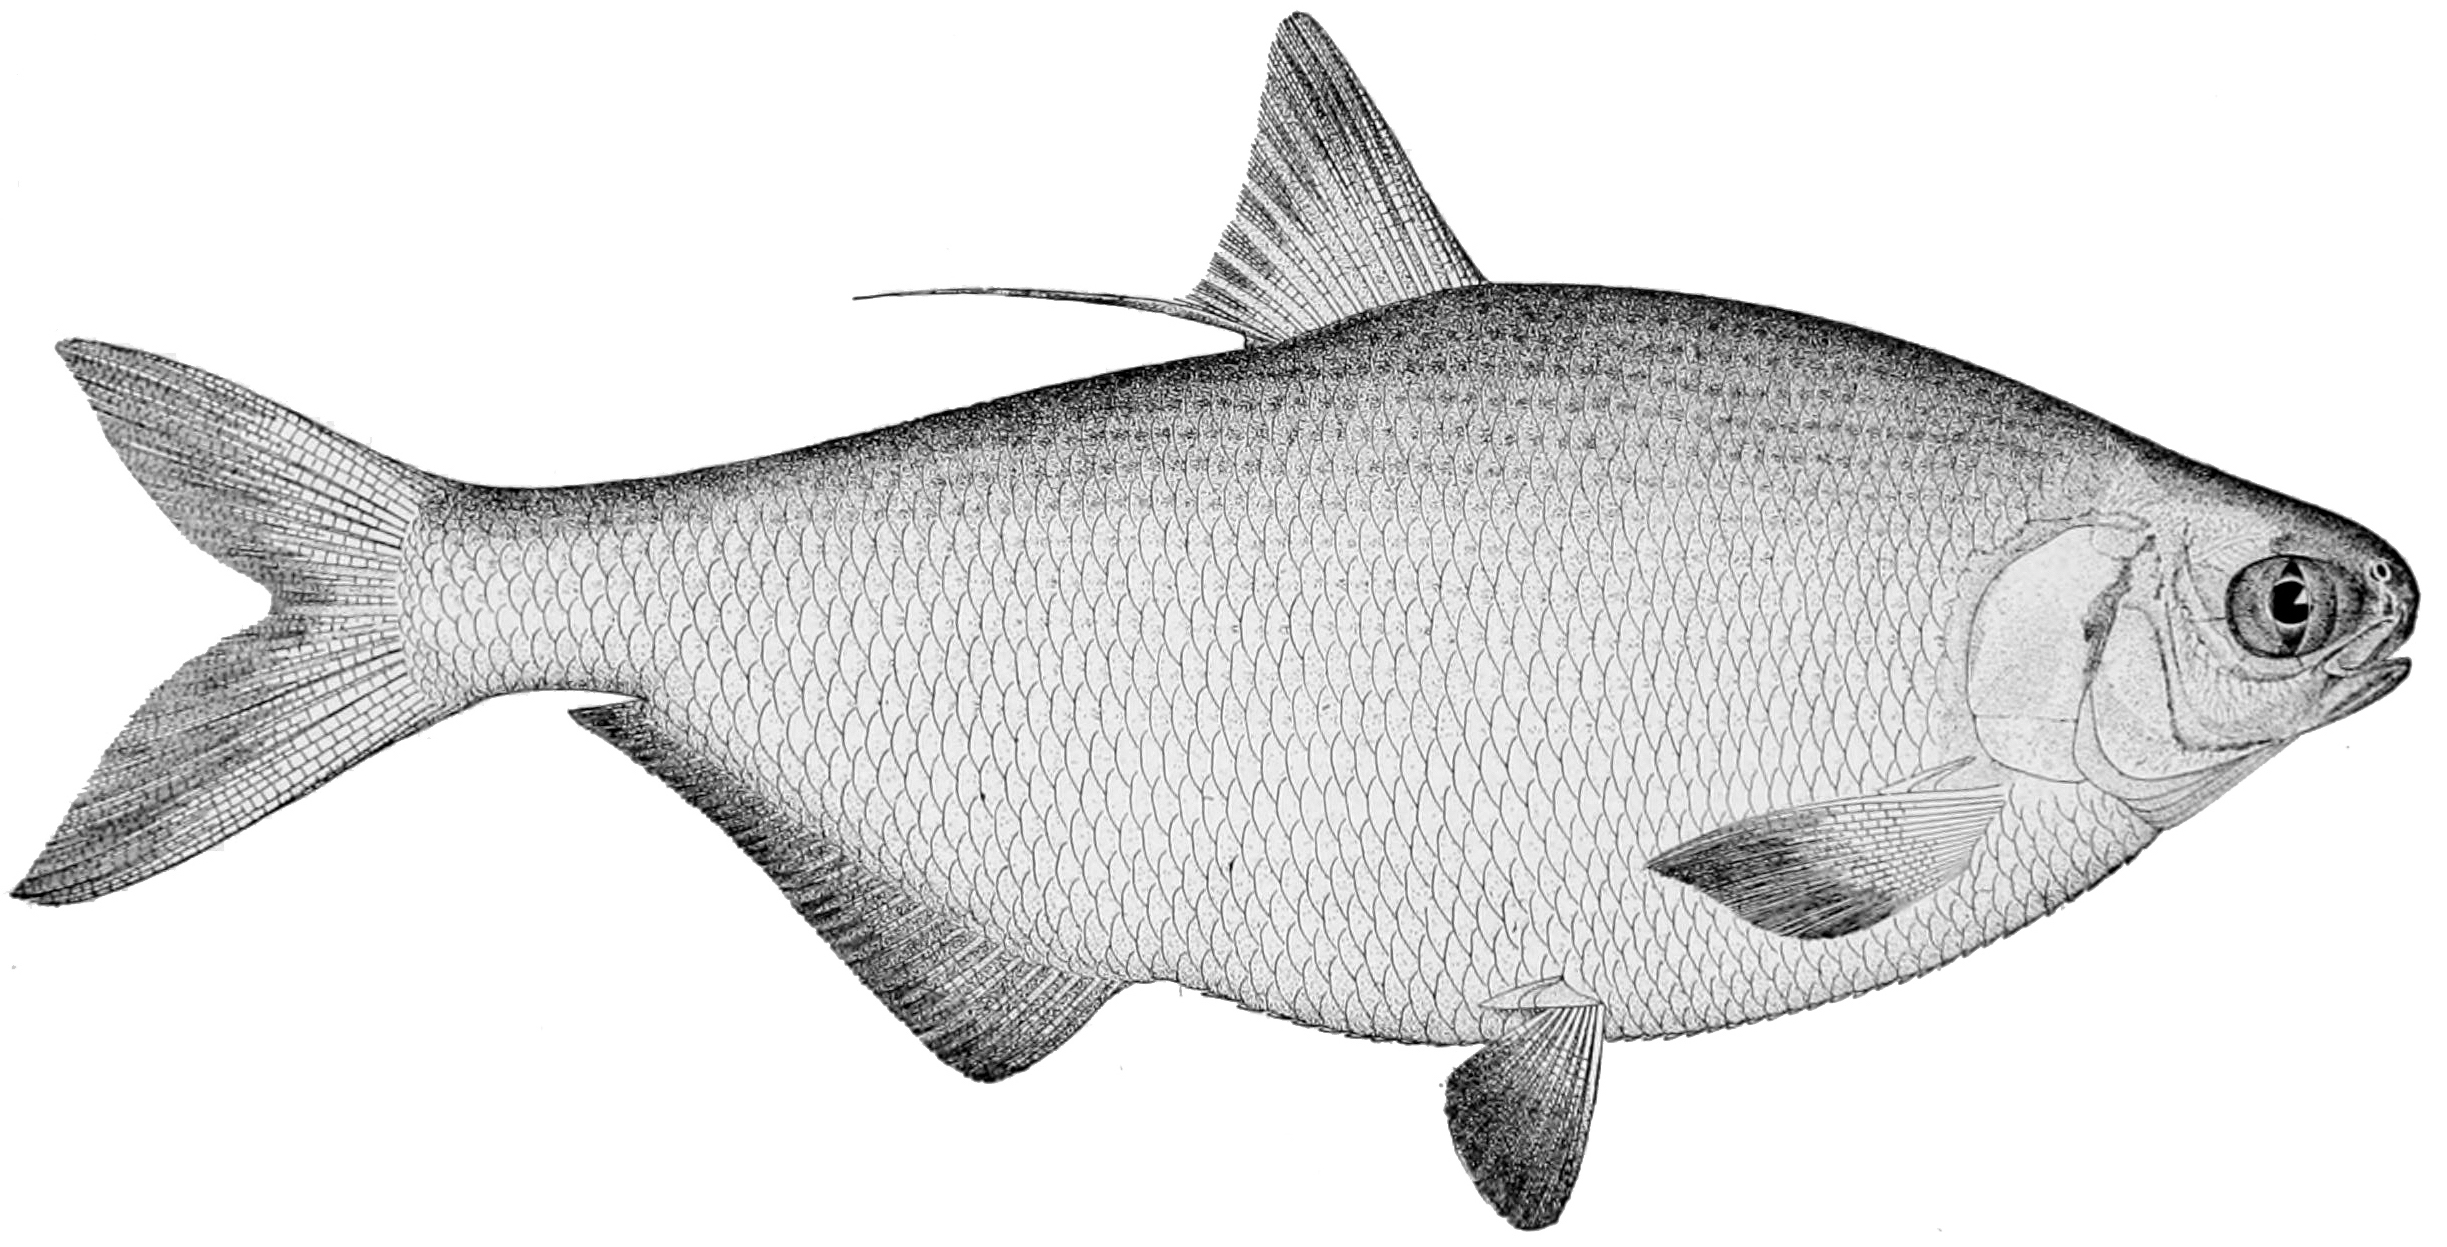
\includegraphics[width=0.15\textwidth]{adult.jpeg}\\
        $n(z',t+1)$};
\node (repro_box) at (13,3.85)  {Reproduction};
\node[align=center] (eggs) at (3,0) {Eggs \\ $\bullet$ $\bullet$ $\bullet$ $\bullet$ \\
  \, $\bullet$ $\bullet$ $\bullet$ $\bullet$ \\ $\bullet$ $\bullet$ $\bullet$ $\bullet$};
  \node[align=center] (eggs_viable) at (5,0) {Viable \\ $\bullet$ $\bullet$ $\bullet$ \\
  \, $\bullet$ $\bullet$ \\ $\bullet$ $\bullet$ $\bullet$};
 \node[align=center] (age1) at (8,0) { Age-1\\
        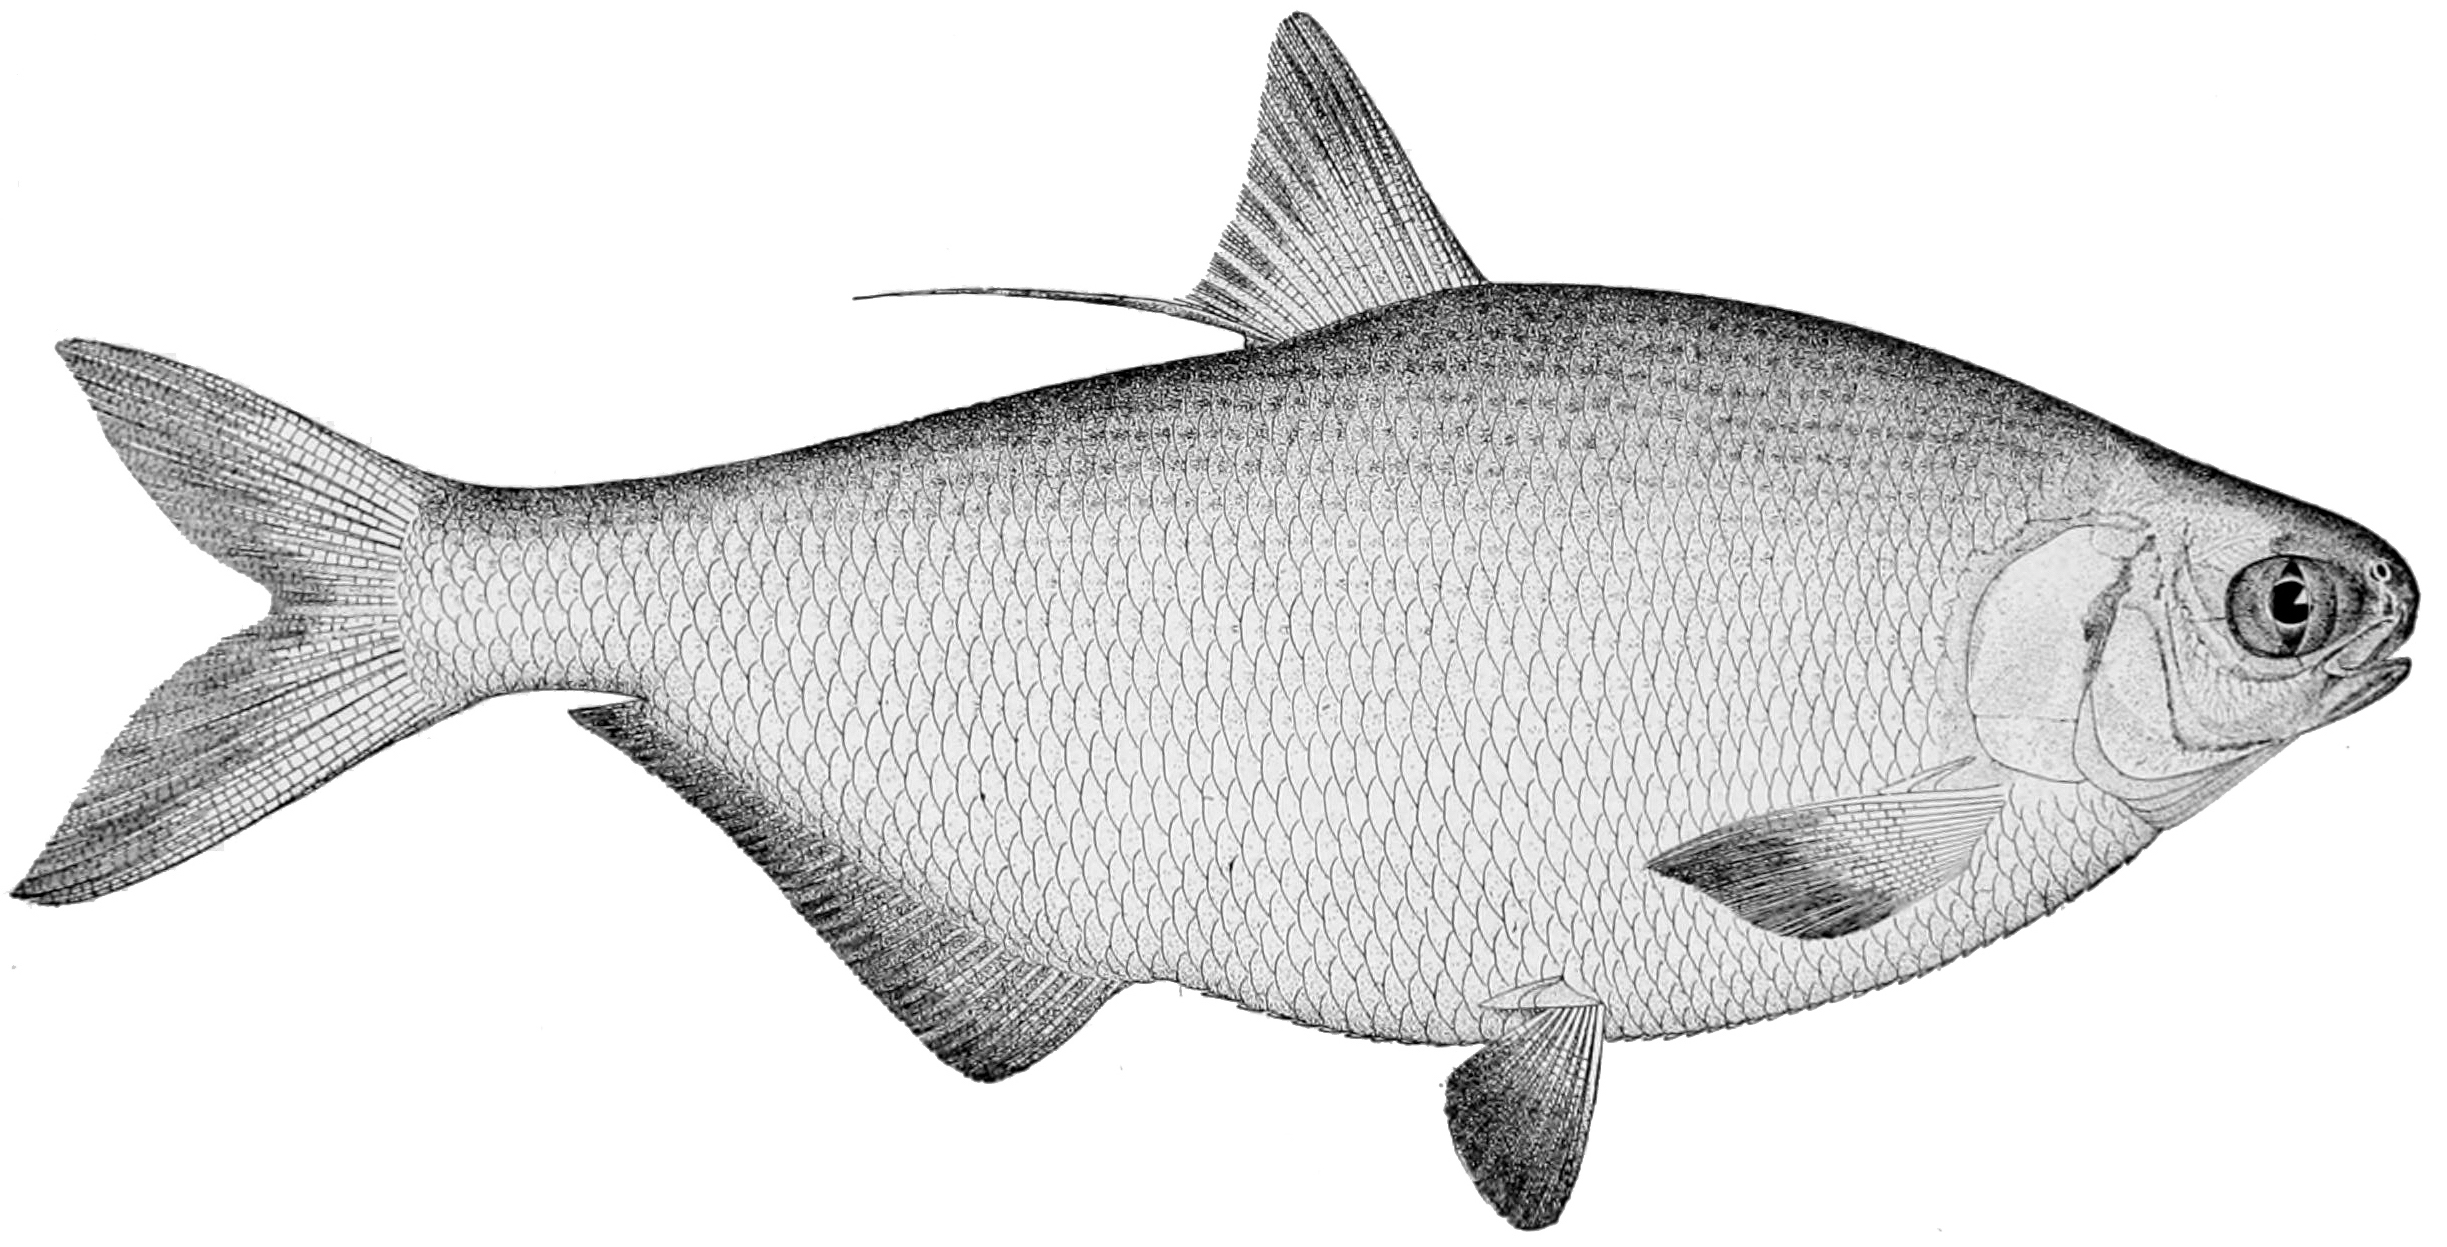
\includegraphics[width=0.06\textwidth]{adult.jpeg}
         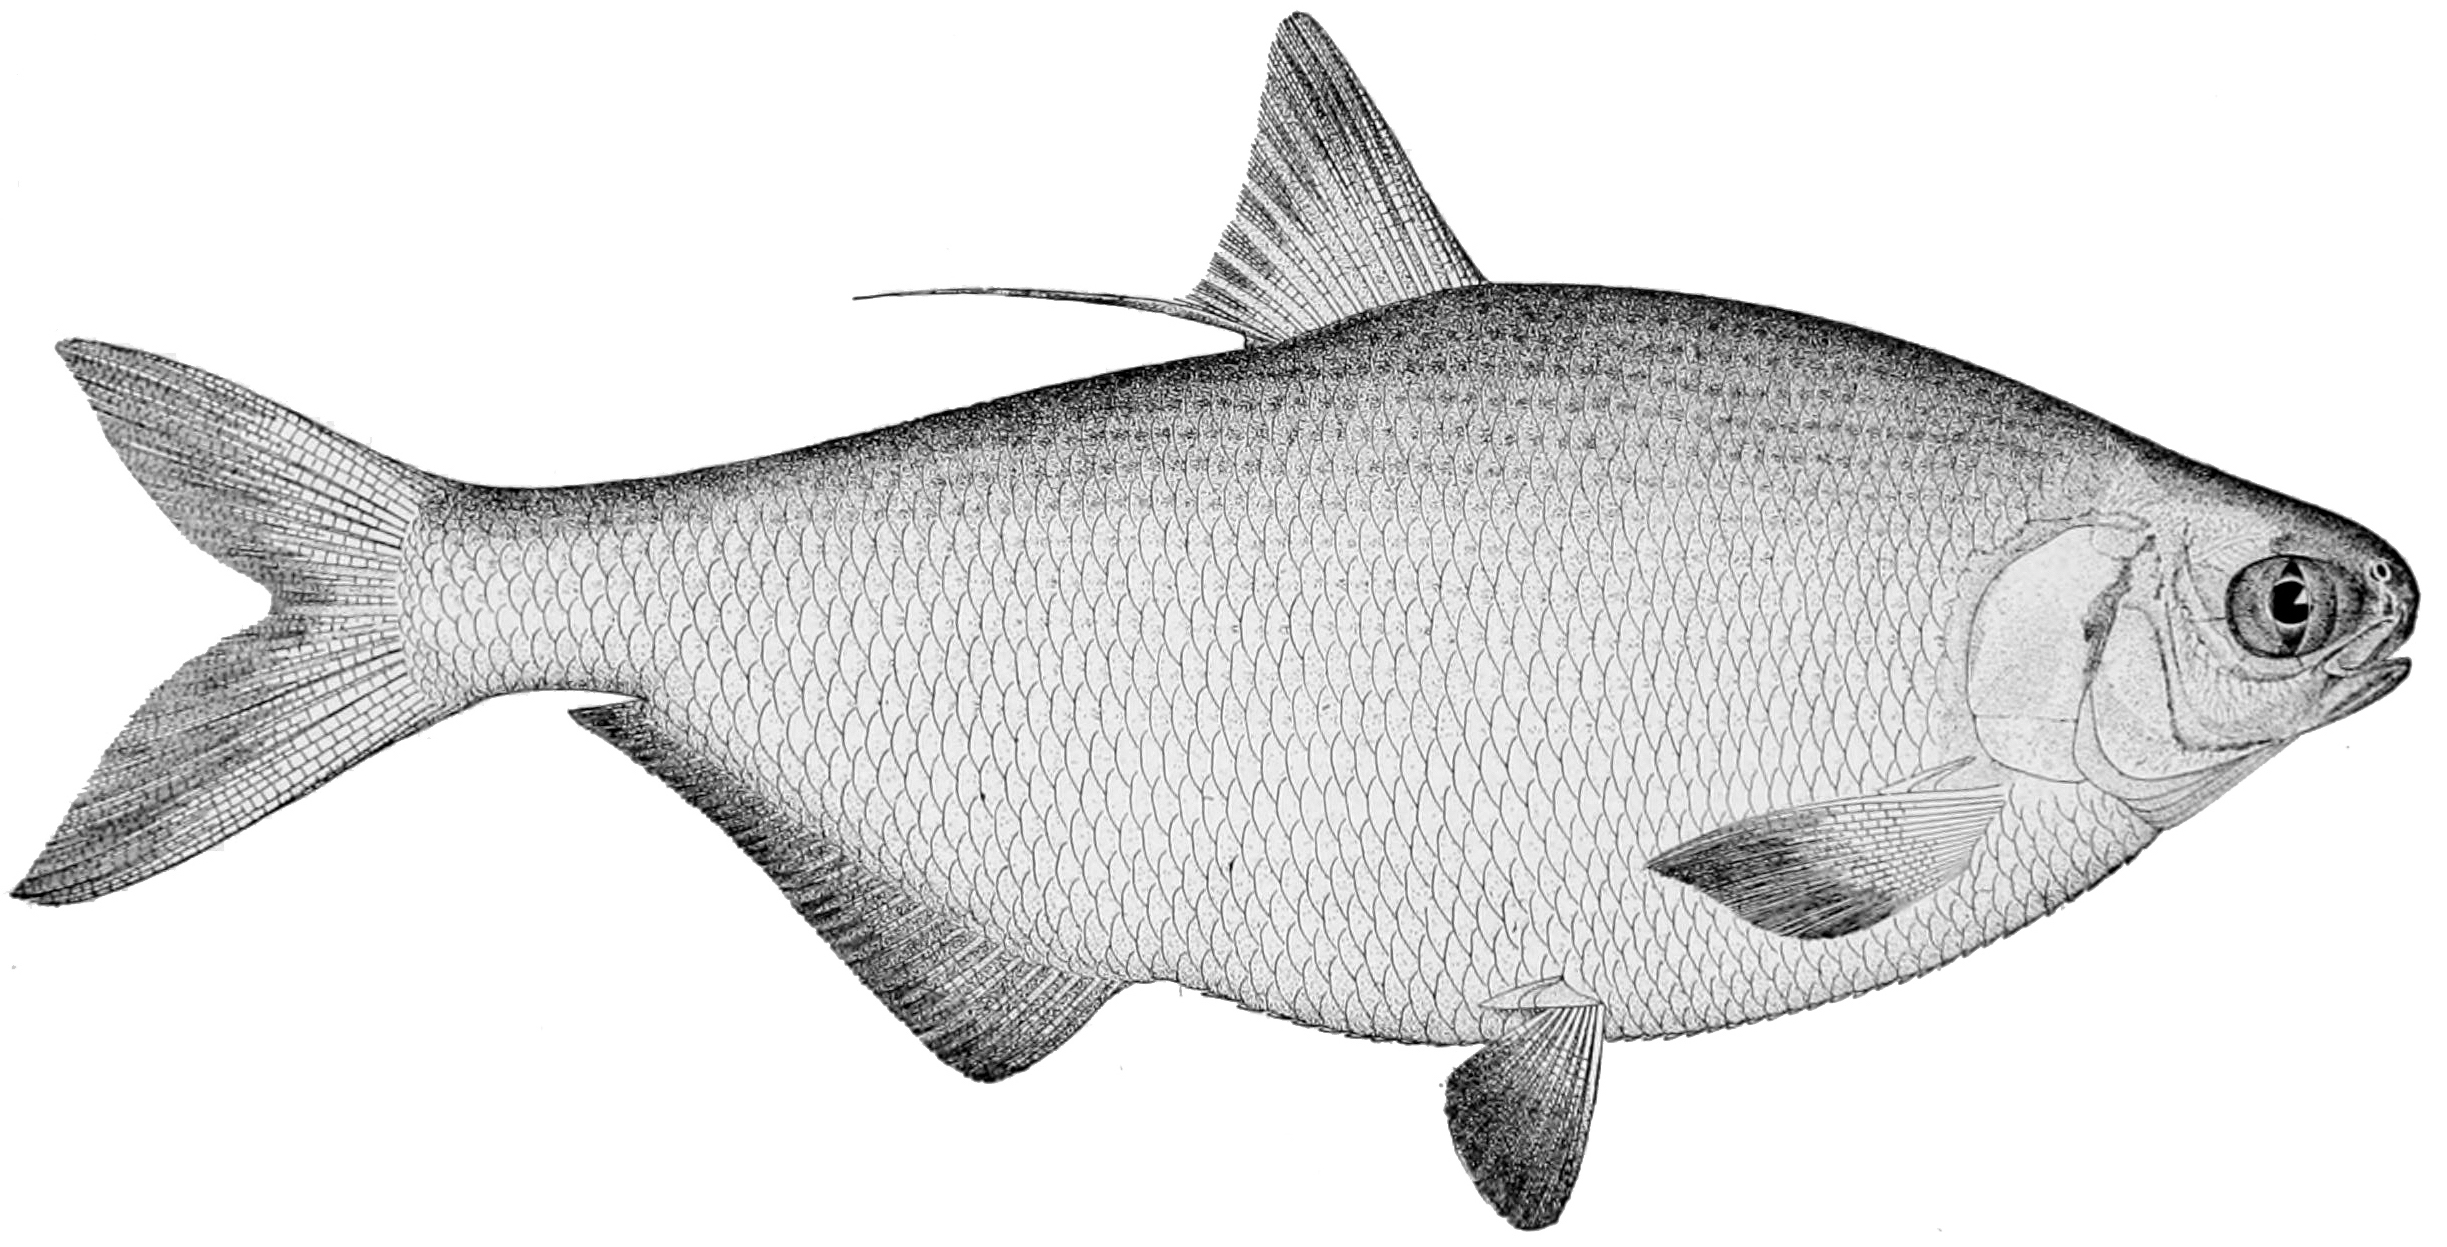
\includegraphics[width=0.04\textwidth]{adult.jpeg}\\
         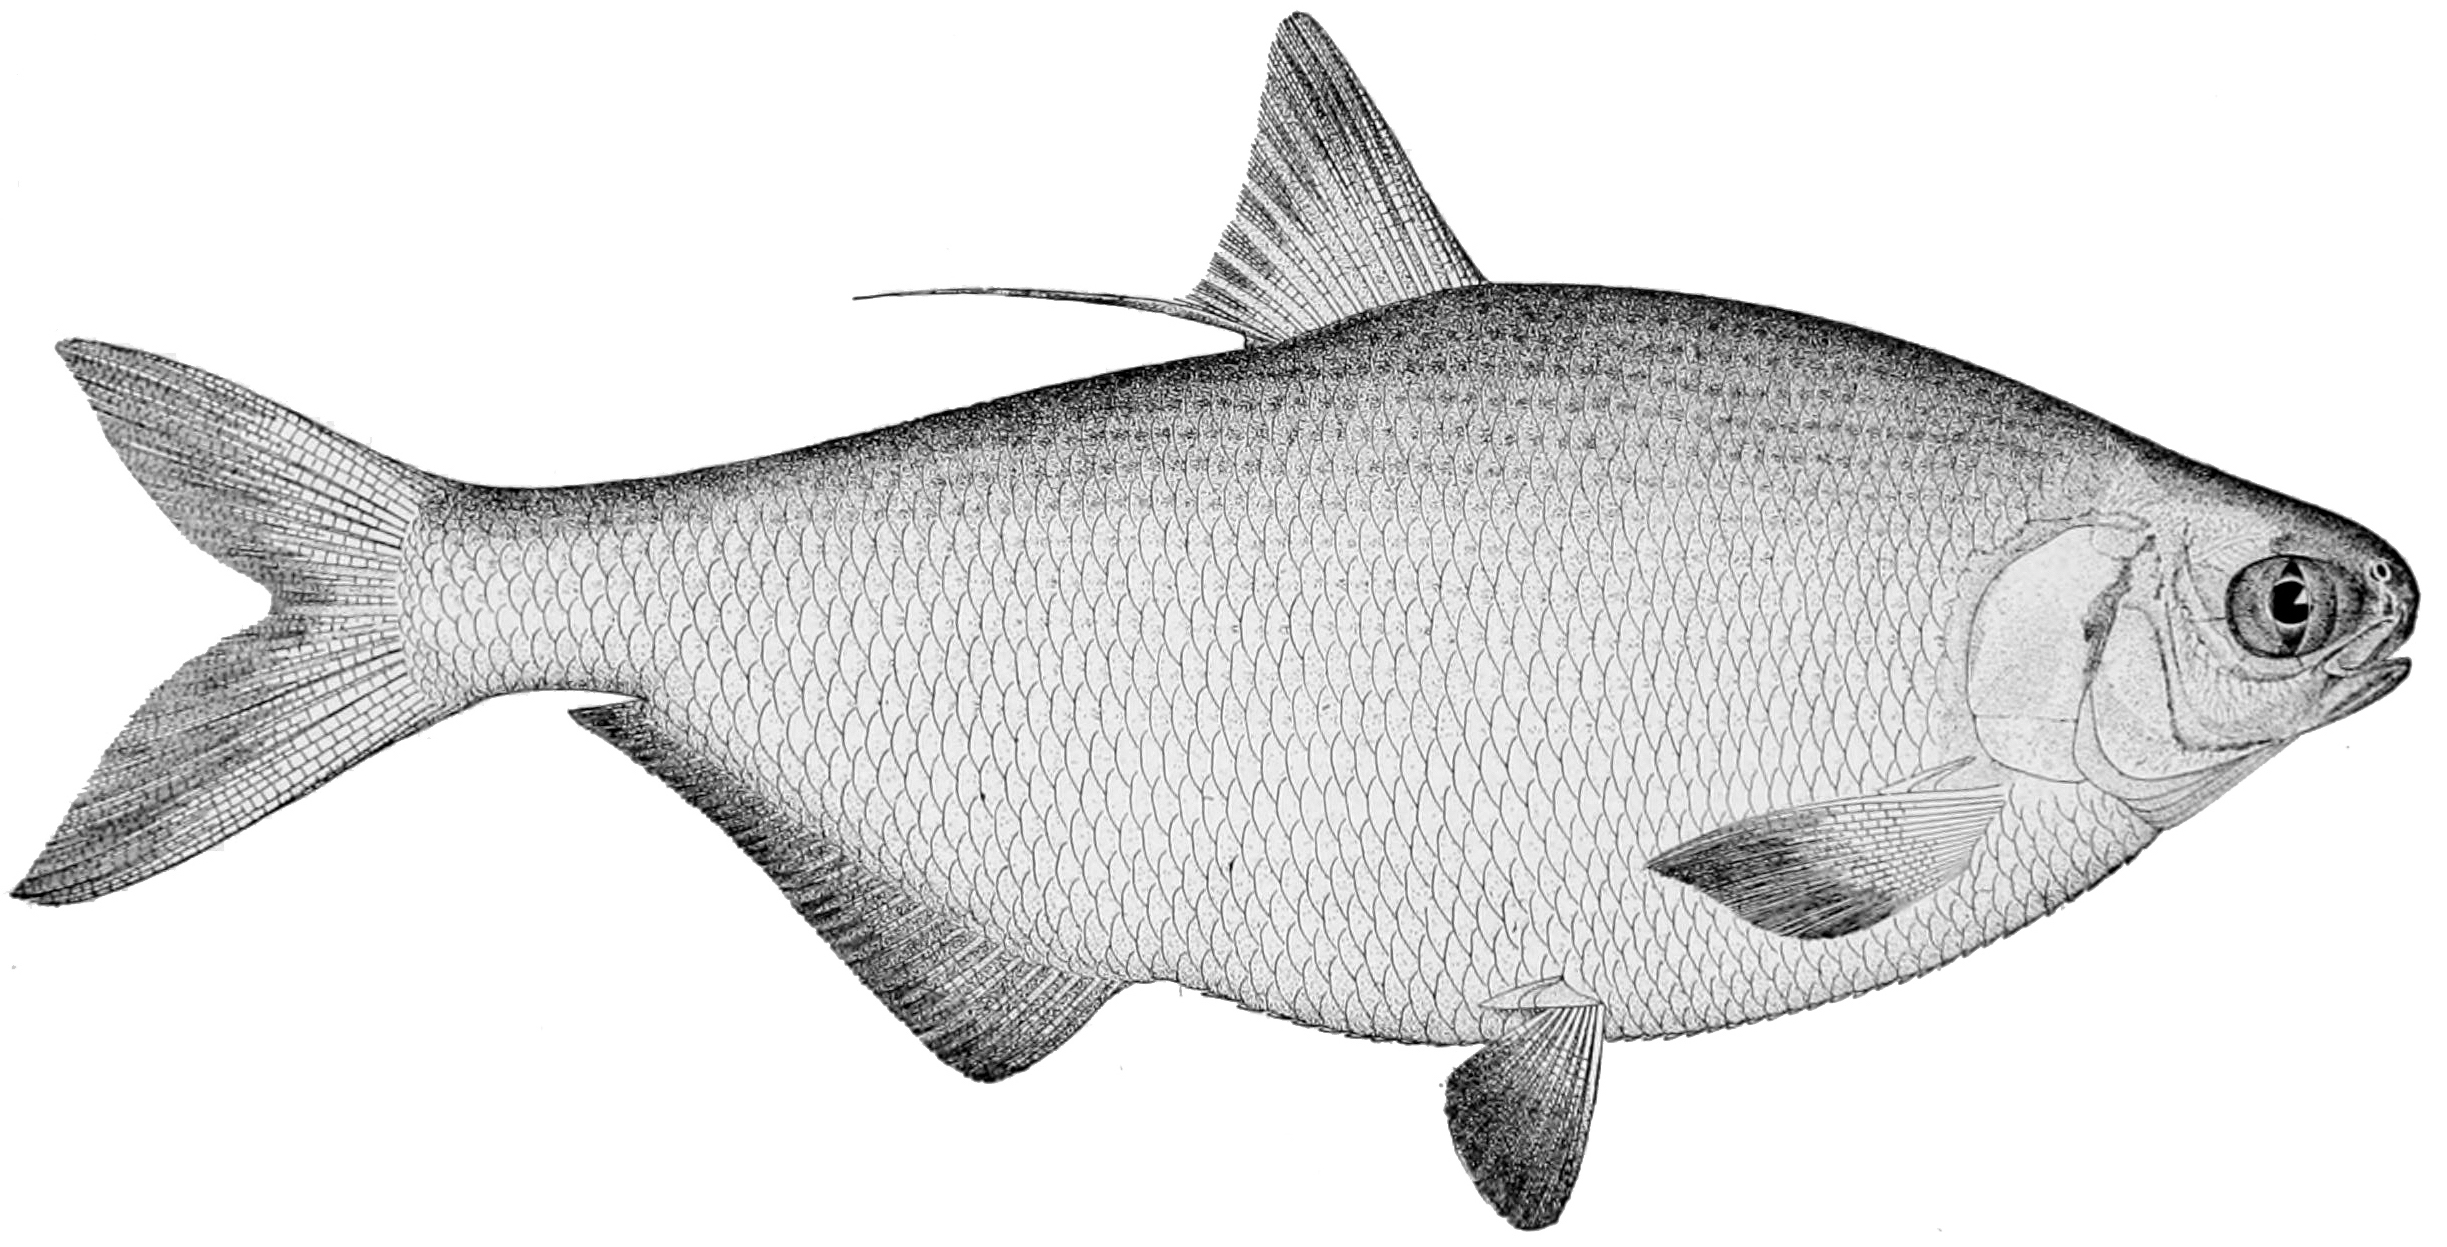
\includegraphics[width=0.08\textwidth]{adult.jpeg}
        };
\node[] (next) at (13,3) {};

\path[->]
	(census_pres) edge node {} (repro_in)
	(repro_out) edge node {$s(z)G(z',z)$} (census_next)
	(census_next) edge node {} (next)
	(repro_down) edge node {$p_b \rm{egg}(z)$} (eggs)
	(eggs) edge node {$\nu$} (eggs_viable)
	(eggs_viable) edge node {$s_0(d)$} (age1)
	(age1) edge node[right, pos=0.3] {$C_1(z')$} (census_next);
	
\end{tikzpicture}
%}
\end{center}
 \caption{\small{Life cycle diagram and census points for pre-reproduction census of gizzard shad.}}
\end{figure*}

\subsubsection{Growth and survival}
We define $P(z'z) = s(z,T)G(z',z)$ where $s(z)$ is the adult annual survival probability and $G(z',z)$ describes the annual length transitions. 
We assumed that the survival function is a logistic function,
\begin{equation}\label{eq:surv}
s(z,T) = s_{\rm min} + \frac{s_{\rm max}-s_{\rm min}}{1+e^{\beta_s(\ln(z)-\ln(\alpha_s)),}}.
\end{equation}
with four parameters: the minimum survival rate $s_{\rm min}$; a maximum survival rate, $s_{\rm max}$; and intercept parameter, $\alpha_{s}$; and a slope parameter, $\beta_{s}$ \citep{bolker2008ecological}.  

We assumed that the growth function is a two-variable normal distribution centered around a modified von Bertalanffy function of the length at time t. 
The von Bertalanffy equation, commonly used to describe the length of a fish over time, is given by $\ds z(t) = L_{\infty} \left(1-e^{-K(t-t_0)} \right)$ where $L_\infty$ is maximum asymptotic length, $K$ is the growth rate, and $t_0$ is the initial time. 
The expected length in the next year
\begin{align*}
 z' =z(t+1) & =  L_{\infty} \left(1-e^{-K(t+1-t_0)} \right) =  L_{\infty} - L_{\infty}e^{-K(t-t_0)} e^{-K} \\
 & =   L_\infty - \left( z(t)-L_\infty \right) e^{-K} =   L_{\infty} \left(1-e^{-K} \right) + z(t)e^{-K}. 
 \end{align*}
Consequently, we assumed that 
%\begin{equation}\label{eq:grow}
$\ds G(z',z) = \mathrm{Prob}(z' \, | \,  z, L_{\infty}, K_g) = \mathrm{Normal PDF}(\mu_g, \sigma_g)$
%\end{equation}
where $K_g$ is the individual growth rate, $\mu_g =  L_{\infty} \left(1-e^{-K_g} \right) + z(t)e^{-K_g}$, and $\sigma_g$ is the standard deviation.

\subsection{Fecundity}
We define the fecundity kernel, 
\begin{equation}\label{eq:fecundity}
F(z', z) = p_b \, \mbox{egg}(z) \, \nu \, s_0(n(z,t)) \, C_1(z')
\end{equation}
where $p_b$ is the probability of reproducing, $\mbox{egg}(z)$ is the mean number of eggs produced, $\nu$ is the probability that an egg is viable, $s_0(n(z,t))$ is the density-dependent probability of surviving to age-1, and $C_1 (z')$ is the length distribution of new recruits at age-1 (when they are first censused).

We assumed that the mean number of eggs produced by females of a certain length is a three-parameter logistic function,
\begin{equation}\label{eq:egg}
\mbox{egg}(z) = \frac{\mbox{egg}_{\rm max}}{1+e^{\beta_e(\ln(z)-\ln(\alpha_e)),}}.
\end{equation}

The probability of survival of gizzard shad during their first year may depend on many factors \citep{michaletz2010overwinter} such as mean temperature, mean total length, the present density of age-0 fish.  
In this study, we focus only on the density factor and define the probability of survival of age-0 fish as the exponential function
\begin{equation}\label{eq:s0}
s_0(d(t)) = a_0 \, e^{-b_0 d(t)}
\end{equation}
where $a_0$ is the intercept, $b_0$ the decay rate, and $d(t)$ is the density at time $t$ of age-0 gizzard shad per 1000 m$^3$, 
\[ d(t) = 10^{-3} \int_L^U p_b \, \mbox{egg}(z) \, \nu n(z,t) \, dz. \]  

Finally, after computing the total number of viable eggs produced and survive to age-1 fish, we multiplied this number with a normal distribution of length,
$ \ds C_1 (z') =  \mathrm{Normal PDF} (\mu_r, \sigma_r)$ where $\mu_r$ is the mean length of age-1 gizzard shad and $\sigma_r$ is the standard deviation. 

\subsection{Dynamical Model} 
%In traditional matrix population models, the state vector is multiplied on the left by a matrix to project the current measurement to its future value.  In an integral projection model, the projection matrix is replaces by an integral kernel $K(z',z)$ that projects the population forward in time.  
The population at time $t+1$ is the sum of the contributions from each individual alive at time $t$,
\begin{equation}\label{eq:IPM}
n(z',t+1) = \int_L^U K(z',z)n(z,t) \,dz,
\end{equation}  
where $K(z',z) = s(z) G(z',z) + F(z',z)$ and $[L,U]$ is the range of all possible lengths.

\section{Methods}
\subsection{Study Area and LTRMP Data Collection}
The 129 km long La Grange Reach is located between La Grange Lock and Dam (L\&D) and Peoria L\&D on the Illinois River, U.S., and is about midway between the Mississippi River and Lake Michigan. 
The Illinois River is a major tributary of the Mississippi River, draining nearly two-thirds of the state of Illinois. 
Along with the main channel of the UMR, the fish community of La Grange Reach has been monitored by the Long-term Resource Monitoring Program (LTRMP) from 1990 to the present, with approximately 500 random collections each year from 15 June to 31 October. 
The LTRMP fish collection methodology included a multiple gear approach (netting and electrofishing) to monitor the general fish community of the UMR system through time \citep{gutreuter1995long}. 
The total lengths were recorded for all fishes captured. 
Methodology, protocols and modifications to the LTRMP can be found in \cite{gutreuter1995long}, and \cite{ickes2002evaluation}. 

The location of La Grange Reach has two important features motivation its choice for the methods of our study. 
First, we parameterized the IPM using data from the main channel of the UMR.  As a part of Illinois River and UMR, La Grange Reach is upstream from the main channel (should we include figure/map?).  
The proximity to, but relative independence from, the main channel, made it a good choice.  Secondly, La Grange Reach is a large pool between the main channel of the Mississippi River and Lake Michigan.  
In recent years, there have been concerns with the threatening introduction of invasive carp to the Great Lakes.  
Consequently, the impact of invasive carp on the native fish populations in the pools leading to the Great Lakes have received an elevated level of attention.  
Understanding the population dynamics of gizzard shad, may in the future make it easier to assess the impacts carp has on native fish populations.

\subsection{Parameterization}
The parameters for the growth function were chosen as the mean values published on a study of gizzard shad located in large impoundments \citep{michaletz2017variation}. 
The survival rate of adults gizzard shad dependent on their length is not well documented and required us to make some additional modeling assumptions.  
An investigation of gizzard shad in Lake Eerie (\cite{bodola1955life}) provided the minimum and maximum survival rate of adults. 
We used a least squares method to find the $\alpha_s$ and $\beta_s parameters that 
minimized the total square-distance between the (observed) pre-carp LTRMP length distribution in the main channels of the UMR (pools 4, 8, 13, 26, and the open river) and (predicted) model equilibrium, $n(z,100)$.  

\subsubsection{Fecundity and recruitment}
Maturity of female gizzard shad corresponds with lengths of approximately 140 mm and the number of eggs produced increase as the females increase in size \citep{jons1997ovarian}.  
The mean eggs produced per female was described by a three-parameter logistic function (see Figure 1) whose parameters were estimated from data provided in Figure 1a. of \citep{jons1997ovarian}. 

The survival to age-0 was assumed to be dependent on the density of age-0 gizzard shad (Figure \ref{fig:surv_age0}).  
We estimated the exponential parameters using data provided in Table 2 of \citep{michaletz2010overwinter}. 
The parameters for the size distribution of age-1 fish were gleaned from a study of gizzard shad located in large impoundments \citep{michaletz2017variation} and the historic 1990-2020 LTRMP dataset of gizzard shad in La Grange Reach.

\begin{figure}
\centering
\begin{subfigure}[b]{.43\textwidth}
  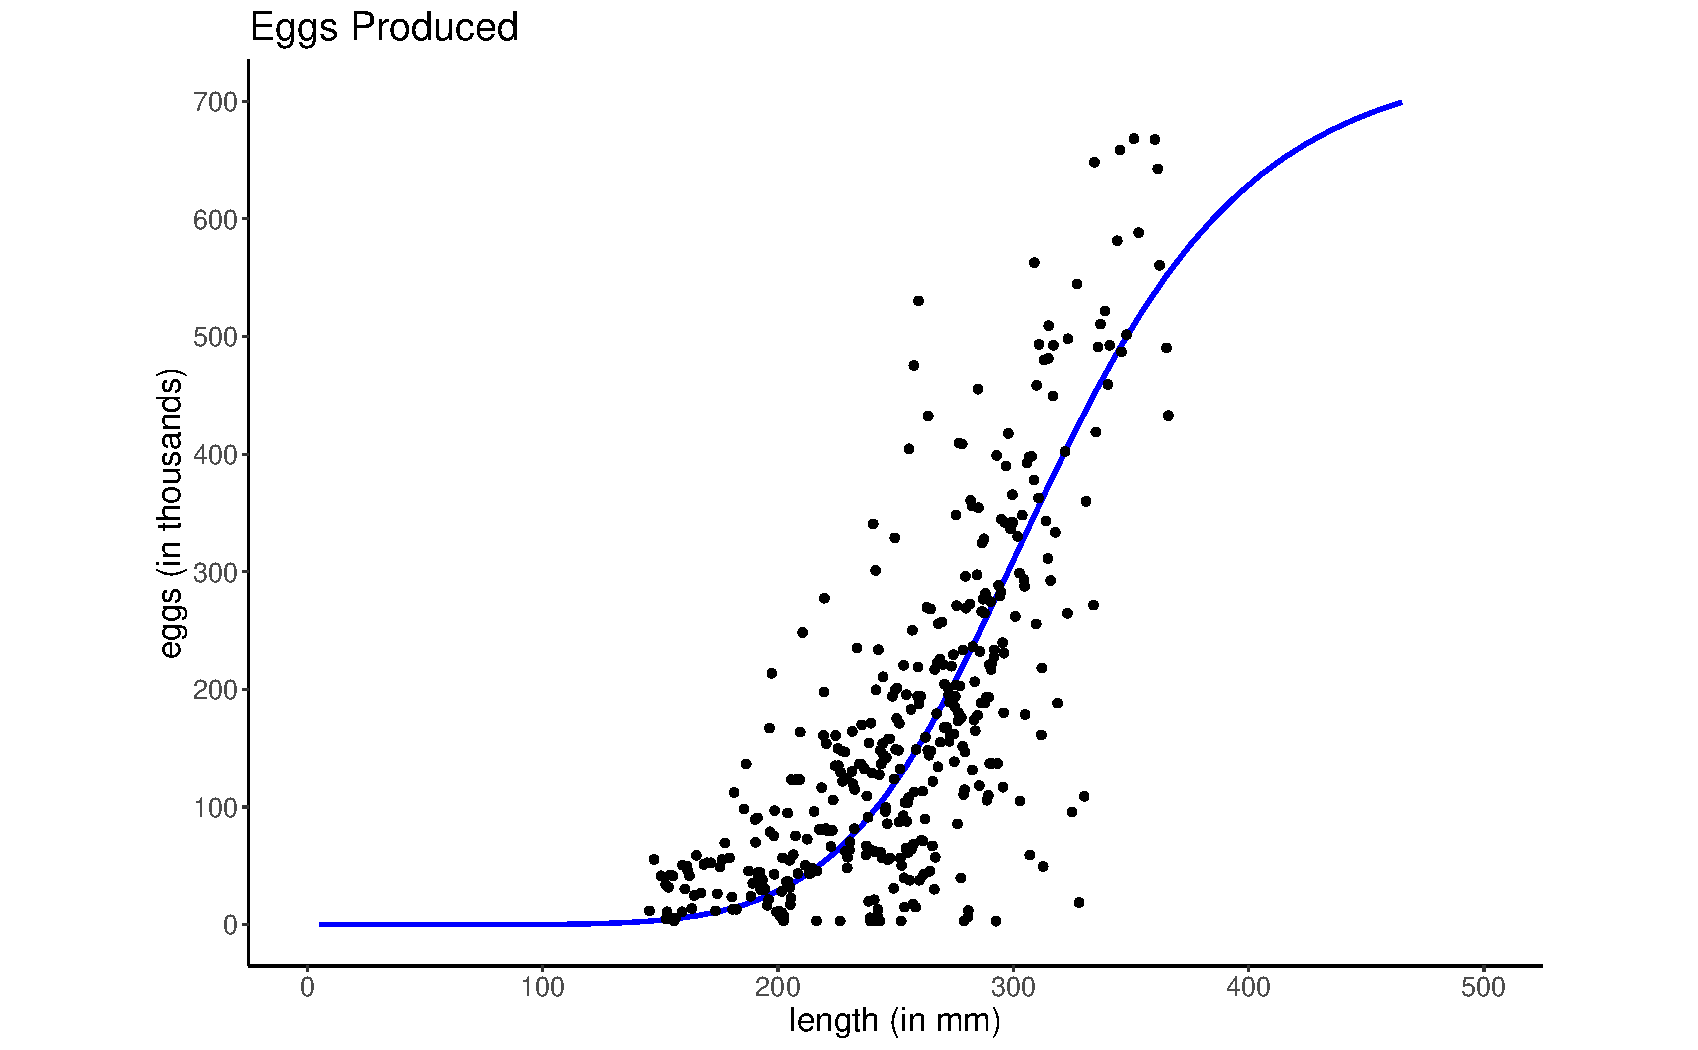
\includegraphics[width=\textwidth]{figures/Figure1a.pdf}
  \caption{}
  \label{fig:eggs}
\end{subfigure}
\begin{subfigure}[b]{.43\textwidth}
  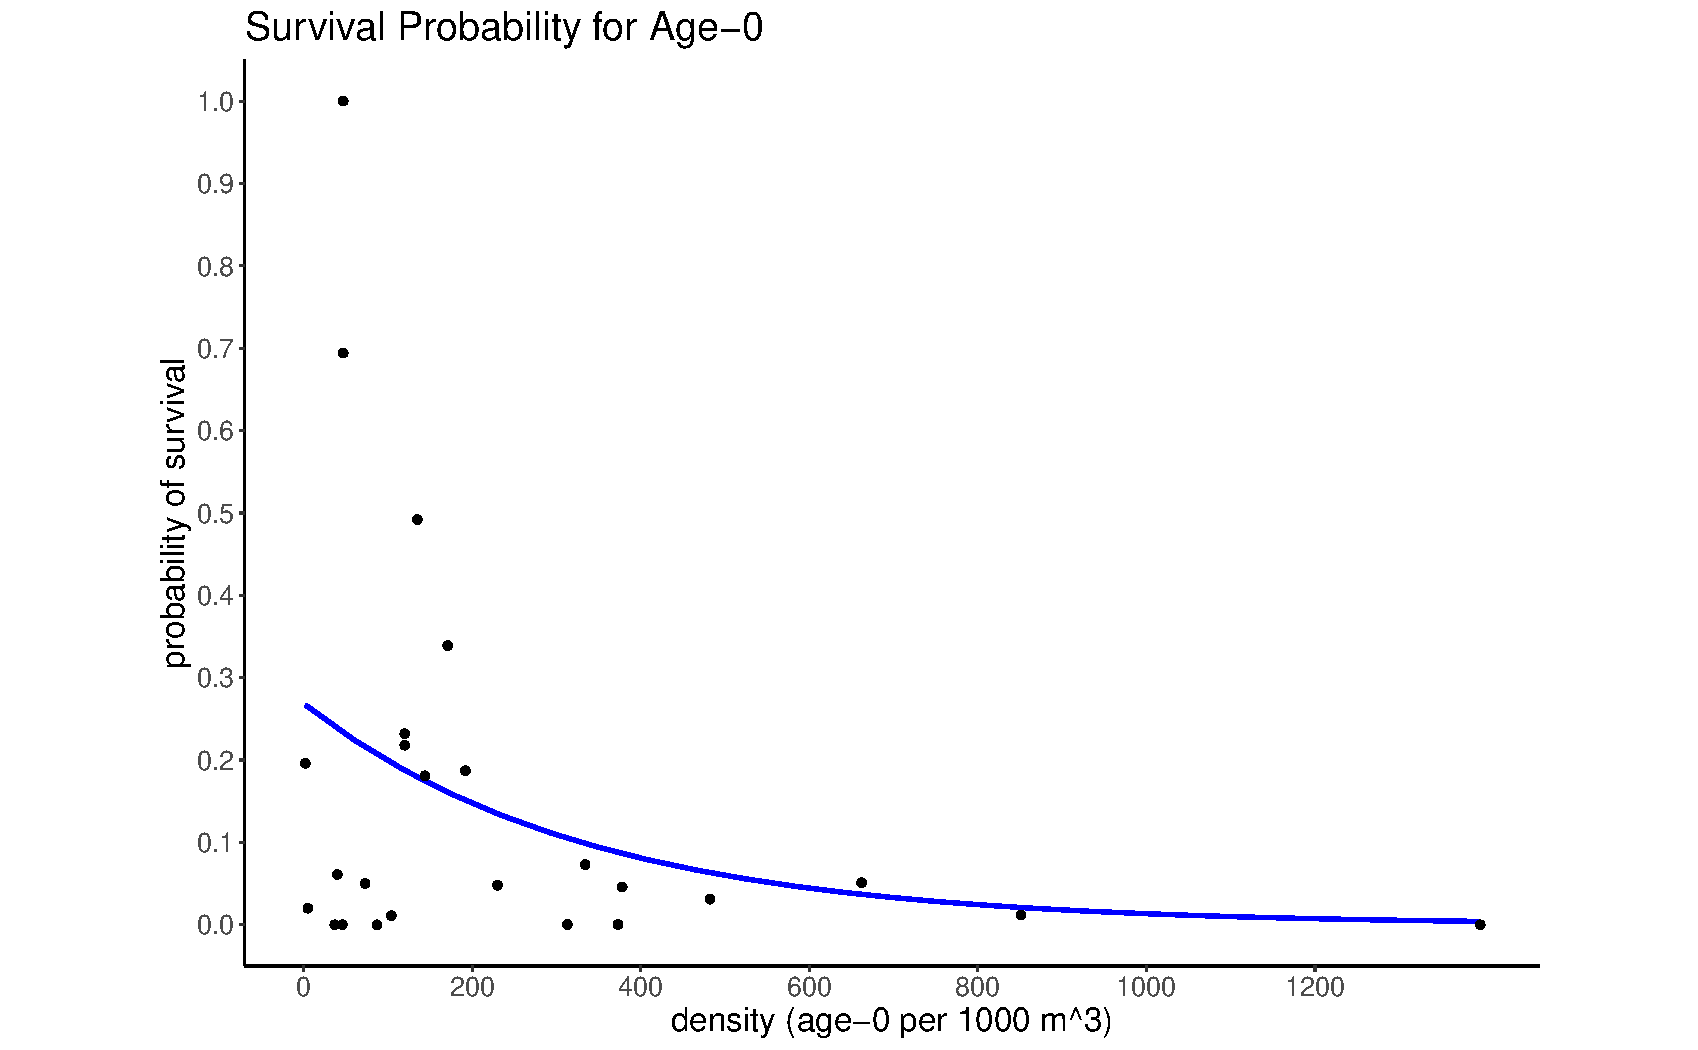
\includegraphics[width=\textwidth]{figures/Figure1b.pdf}
  \caption{}
  \label{fig:surv_age0}
\end{subfigure}
\caption{(a) Graph of $\mbox{egg}(z)$. Data from \citep{jons1997ovarian}.  (b) Graph of $s_0(d)$. Data from \citep{michaletz2010overwinter}. }
\label{fig:fecundity}
\end{figure}    
%
%To complete the recruitment process we assign a length to the recruited individuals by simulating a Gaussian random variable with mean $\mu_c$ and standard deviation $\sigma_c$.

\section{Analysis and Results}
We numerically solved the integral model using the Midpoint Rule with large approximating matrices \citep{burden2005numerical}. 
The Midpoint Rule has been commonly used for integral projection models because of its simplicity and effectiveness \citep{ellner2006integral, ramula2009integral,  merow2014advancing}. 
During the course of model development, we explored different step sizes for the Midpoint Rule and found that about 50 points provided numerically stable results. 
We integrated over lengths from 0 mm to 400 mm. 
The upper limit was chosen based upon numerical stability and consistency of the system (e.g., avoiding eviction or the loss of individuals due to numerical errors \citep{williams2012avoiding}). 

\subsection{Initial conditions}  We assumed that the initial density of gizzard shad $d_0 = 964.7$, the annual average density of gizzard shad observed in La Grange Reach from 1993-2019.  
The probability of an individual being length $z$ at time $t=0$  was assumed to be normally distributed with mean $0.5L_\infty$ and standard deviation $\sigma_0 = 30$, similar to observations (1990-2020) in LTRMP fish dataset.  
As a result, we initialized our model with
\begin{equation}\label{eq:n}
 n(z,0) = d_0 \mbox{Norm} (0.5 L_\infty, \sigma_0) = 964.7 \mbox{Norm} (166, 30). 
 \end{equation}

The model was coded in R \citep{R} and the scripts are published on JP github page \verb+https://github.com/jppeirce+.

\subsubsection{Comparison with the LTRMP La Grange dataset}
%The only data used in the model from La Grange Reach was the average water temperature during the early Spring period March 15 - April 15 (used to determined the adult survival inflection point).
The total number of gizzard shad in our simulation reached a stable equilibrium (Figure \ref{fig:ntotal}) within 50 years and, more relevantly, the length distribution at that equilibrium compares favorably with the observations from La Grange found in the LTRMP fish dataset (Figure \ref{fig:lagrange}). 
We notice that the peak frequencies are near the same length with the model predicting slightly more adults lengths and fewer juvenile lengths than the observations. 
The location of the maximum in the LTRMP data, corresponding to new recruits, suggests that there may be smaller age-0 fish than in study from \citep{michaletz2017variation} that was used in the model parameterization.  

\begin{figure}
\centering
\begin{subfigure}[b]{.43\textwidth}
  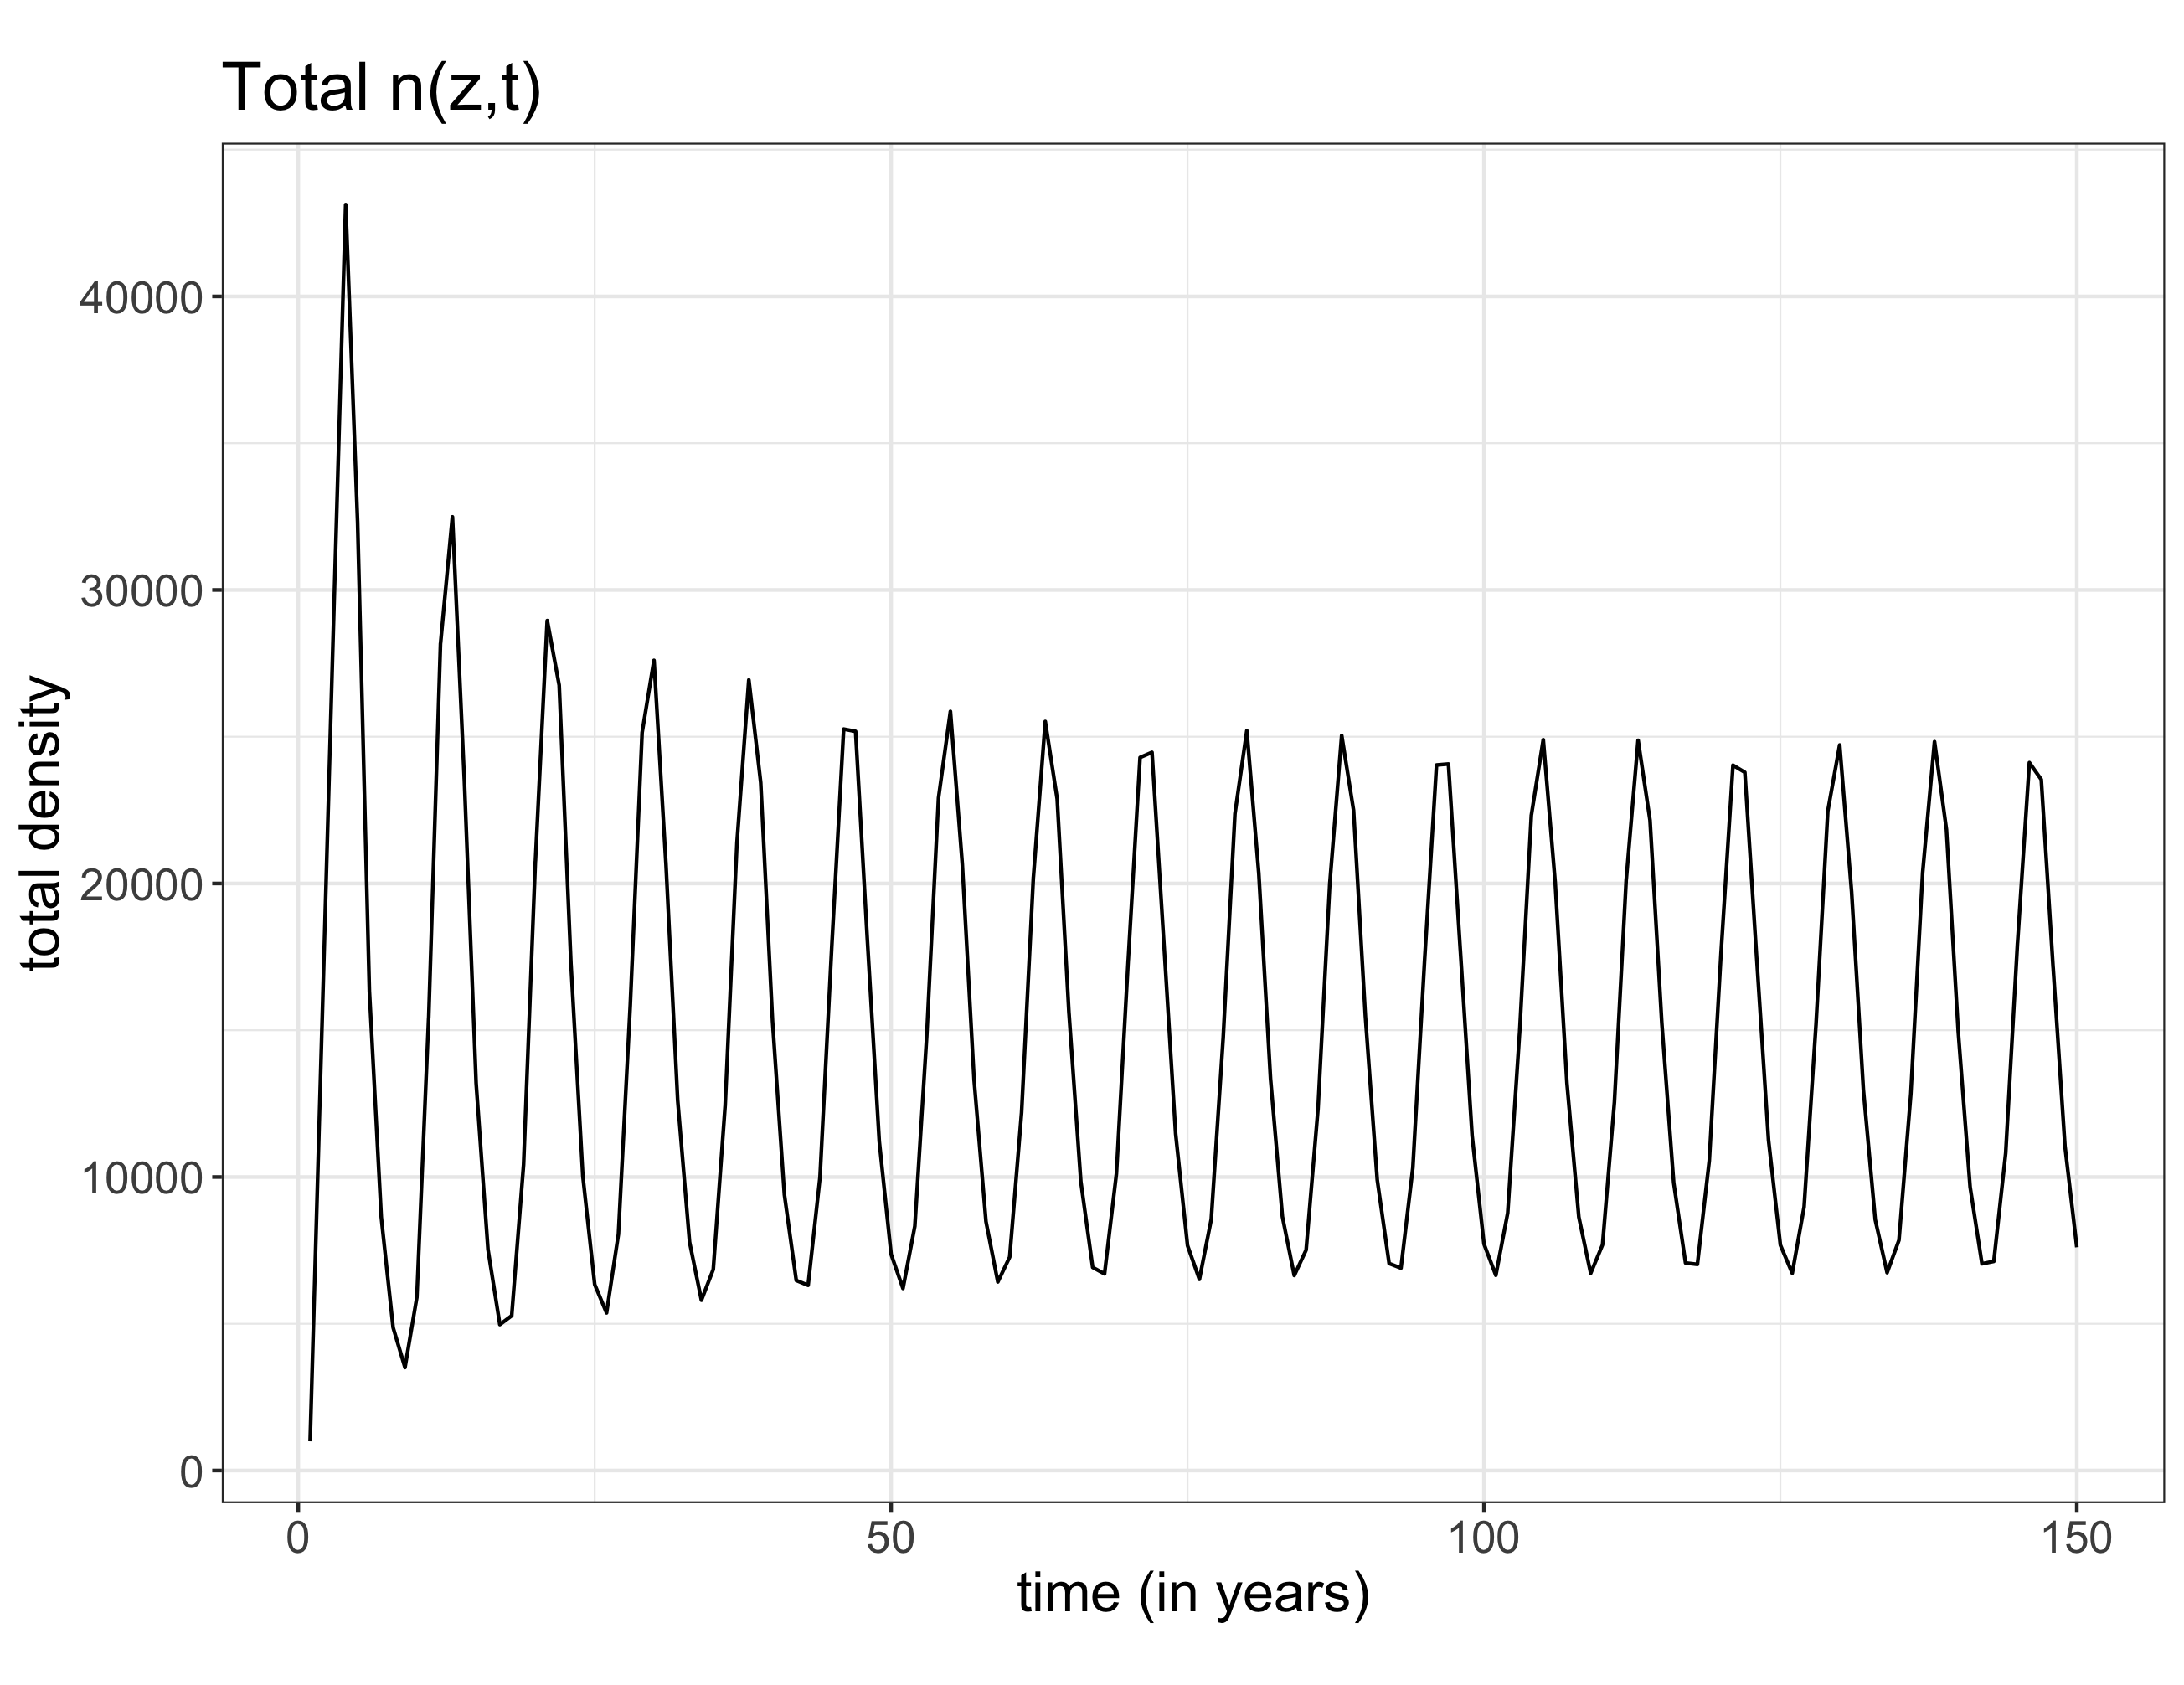
\includegraphics[width=\textwidth]{figures/ntotal.png}
   \caption{}
  \label{fig:ntotal}
\end{subfigure}
\begin{subfigure}[b]{.43\textwidth}
   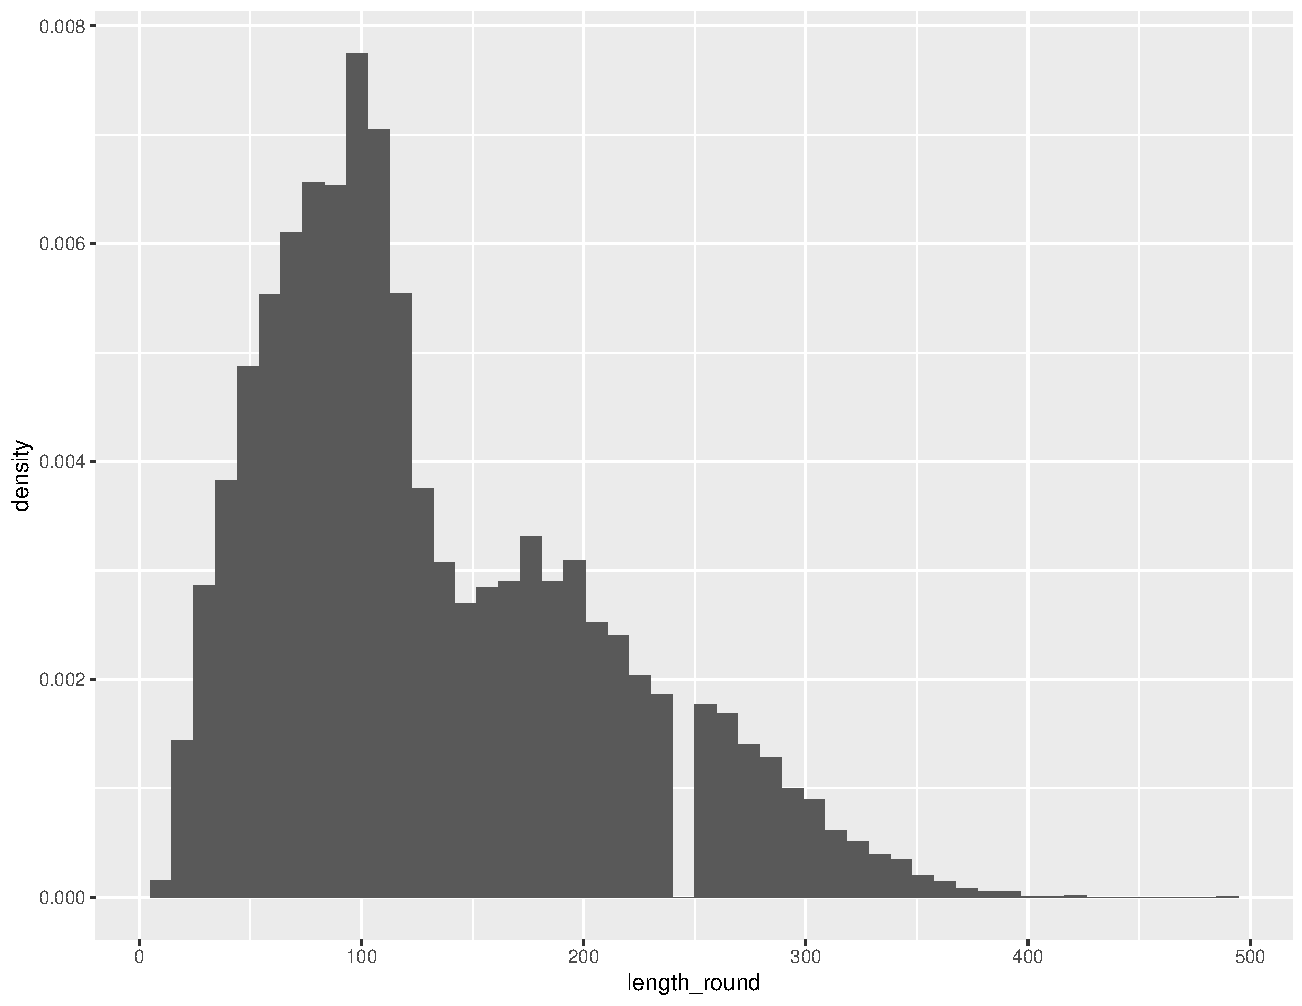
\includegraphics[width=\textwidth]{figures/lagrange.pdf}
     \caption{}
\label{fig:lagrange}
\end{subfigure}
\caption{(a) The total number of gizzard shad in La Grange Reach predicted by IPM for first 50 year. (b) LTRMP observations of gizzard shad in La Grange Reach (histogram with 50 len) compared with the IPM length frequency at equilibrium ($t=100$ years)}
%\caption{(a) Graph of $p_b(z)$ (b) Graph of $\mbox{egg}(z)$, (c) Density-dependent survival of age-0 gizzard shard.}
%\label{fig:fecundity}
\end{figure}    

\subsubsection{Survival and Relative Growth}
The dependence on survival of next generation of age-0 fish on the present density of age-0 fish strongly influences the density, at all ages, of gizzard shad within the population. 
When the fish density is large, there may be more fish at longer lengths and consequently a greater number of eggs produced.  
More eggs leads to a higher density of age-0 fish and reflectively a reduction in the survival to age-1.  
If this reduced survival continues for a few years, the overall density of fish may decline and there may not be as many larger fish reproducing.  
If fewer eggs are spawned, there are less age-0 fish and the reduced density leads to a better survival probability.  
For these years we would expect the overall density to increase.  
This cycle of oscillation continues, reflected in our model by the time-dependent survival probability of age-0 (Figure \ref{fig:age0time}) and the relative growth rate 
$$ \lambda(t) = \left. \int_L^U n(z,t+1) \, dz \middle/ \int_L^U n(z,t) \, dz \right.$$ (Figure \ref{fig:lambda}).

\begin{figure}
\centering
%\begin{subfigure}[b]{.43\textwidth}
  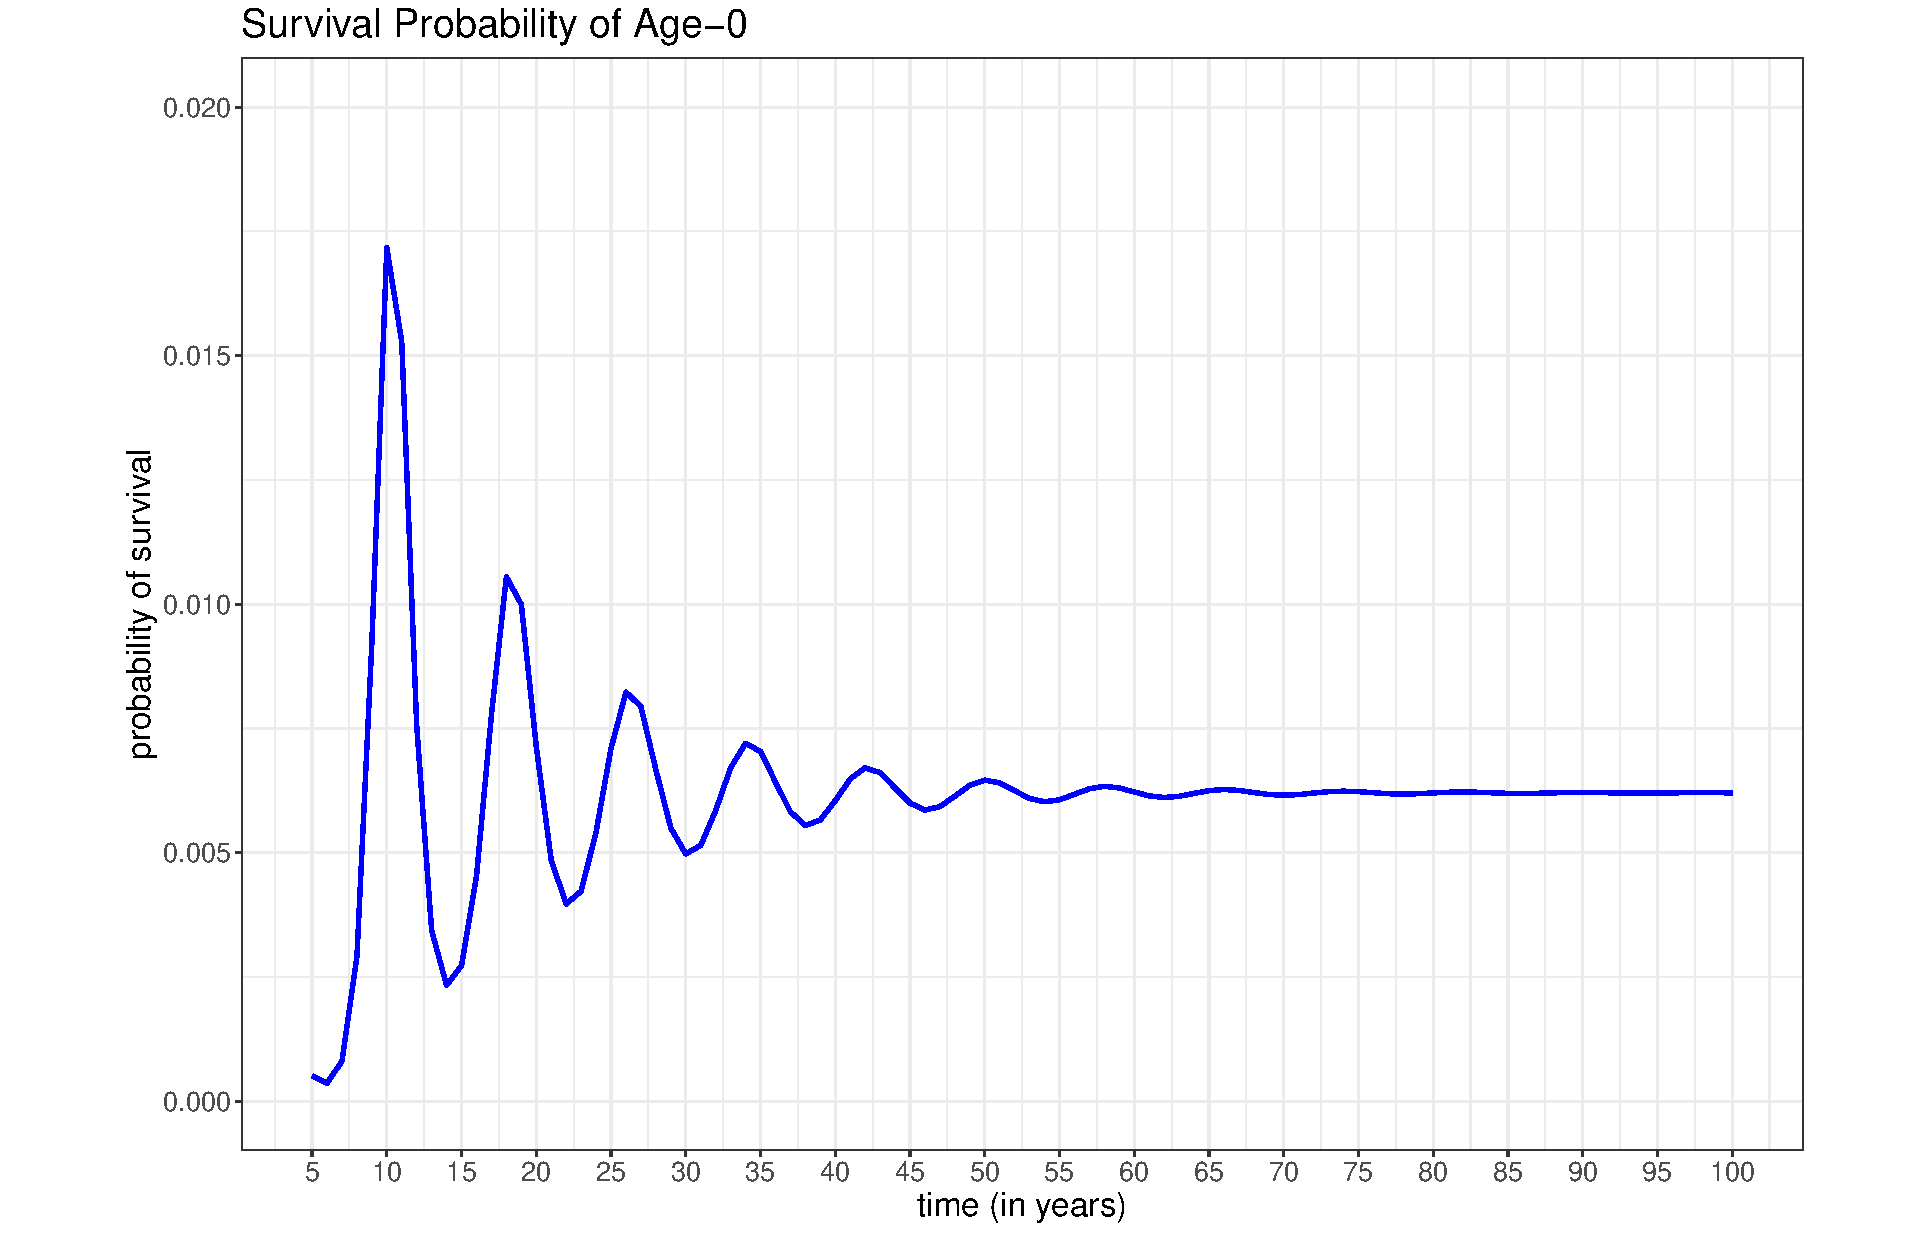
\includegraphics[width=.4\textwidth]{figures/Figure2a.pdf}
   \caption{}
  \label{fig:age0time}
%\end{subfigure}
%\begin{subfigure}[b]{.43\textwidth}
%   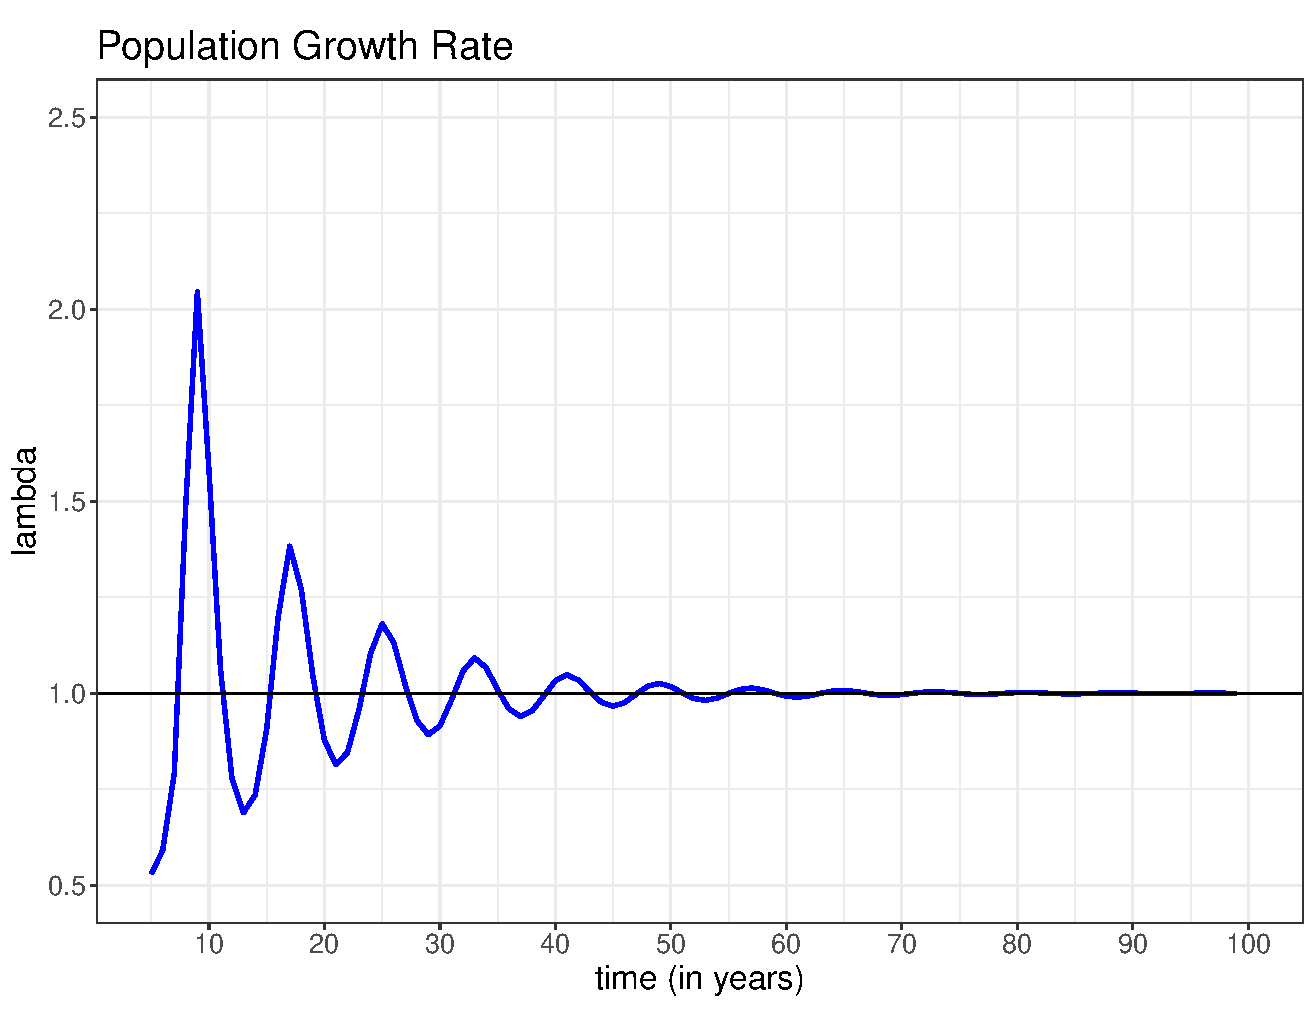
\includegraphics[width=\textwidth]{figures/Figure2b.pdf}
%     \caption{}
%\label{fig:lambda}
%\end{subfigure}
\caption{(a) Survival of age-0}
%\caption{(a) Graph of $p_b(z)$ (b) Graph of $\mbox{egg}(z)$, (c) Density-dependent survival of age-0 gizzard shard.}
%\label{fig:fecundity}
\end{figure}    

\subsection{Time Evolution of Initial State}
Starting with $n(z,0)$ defined by Equation \ref{eq:n}, we computed the length distribution for 3 years.  
In year 1, there are two relative maximum frequencies corresponding to the recruitment of age-1 fish and the survival of the adults.

\subsubsection{Dynamics of the Age-1 Over Time - Fixed Frame}
 The greatest value of $n(z,1)$ during year one is centered at the mean length of recruitment. 
 In the following years, the decrease in the maximum value is a result of the two factors:  the reduction in the density of adults and the density-dependent survival function for age-0 fish. 
 Starting in year 1, there is a reduction in the number of egg-producing adults (lengths above 140 mm) compared with the initial population.  
 From Figure \ref{fig:eggs}, fewer longer adults implies fewer eggs produced.  
 The eggs that are produced, however, may have a greater chance of survival to the age-1 census (Figure \ref{surv_age0}).  
 This is evident in the increase in density of recruits (NEED TO SHOW?) but is illustrated in lower frequency of recruits (Figure \ref{fig:length_dist}) 

%illustrates that this survival advantage is not sufficient to maintain or increase the frequency of recruits.  


% and as a consequence the density of    to lengths centered at approximately 210 mm.  In the following years, there is a decrease in the frequency of the age-0 fish length.  This is caused by two factors resulting from the reduction in the frequency of egg-producing adults (lengths above 140 mm) compared with the initial population. First, is the decline in the numbers of eggs produced.  From Figure XXX, we assumed that longer fish produce more eggs.  As a result, the second factor is the increase in the density of age-0 fish.  As density of age-0 fish increases, the survival rate of age-0 decreases (see Figure XXX).

[Theme: Dynamics of a cohort - moving frame]
Figure XXX also demonstrates the growth in gizzard shad population.  
The peak length frequency of age-1 fish in $n(z,1)$ near $z = 105$ mm is seen as a peak in $n(z,2)$ near 160 mm, and again as a peak in $n(z,3)$ at about 210 mm. 
 MORE DISCUSSION NEEDED

%Two factors influence a reduction in the frequency of age-0 lengths in years 2 and 3. First, there are fewer egg-producing adults (lengths above 140 mm) compared with the initial population.  This cause Second, the density of age-0

%\begin{figure}
%\centering
%  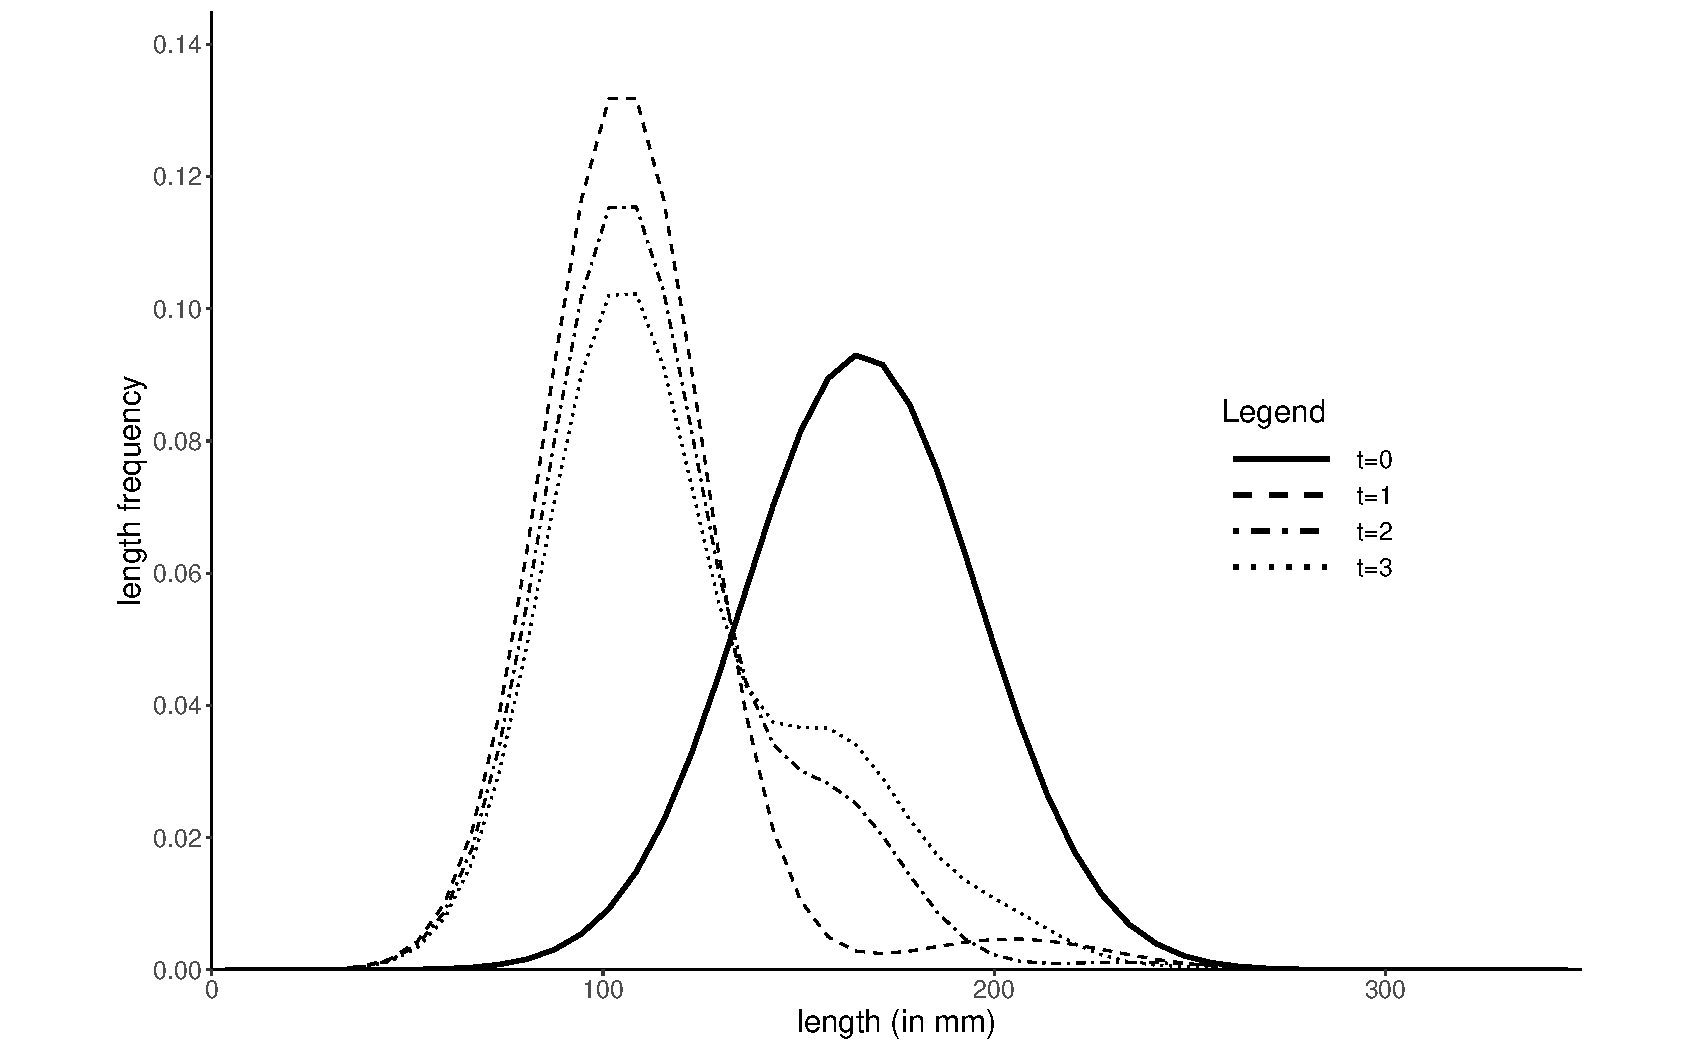
\includegraphics[width=.45\textwidth]{figures/lengthdist.pdf}
%\caption{Simulated frequency of lengths of Gizzard Shad.  Initial density  and N=xxx}
%\label{fig:length_dist}
%\end{figure}   
%
%

\begin{figure*}
\centering
\begin{subfigure}[b]{.43\textwidth}
  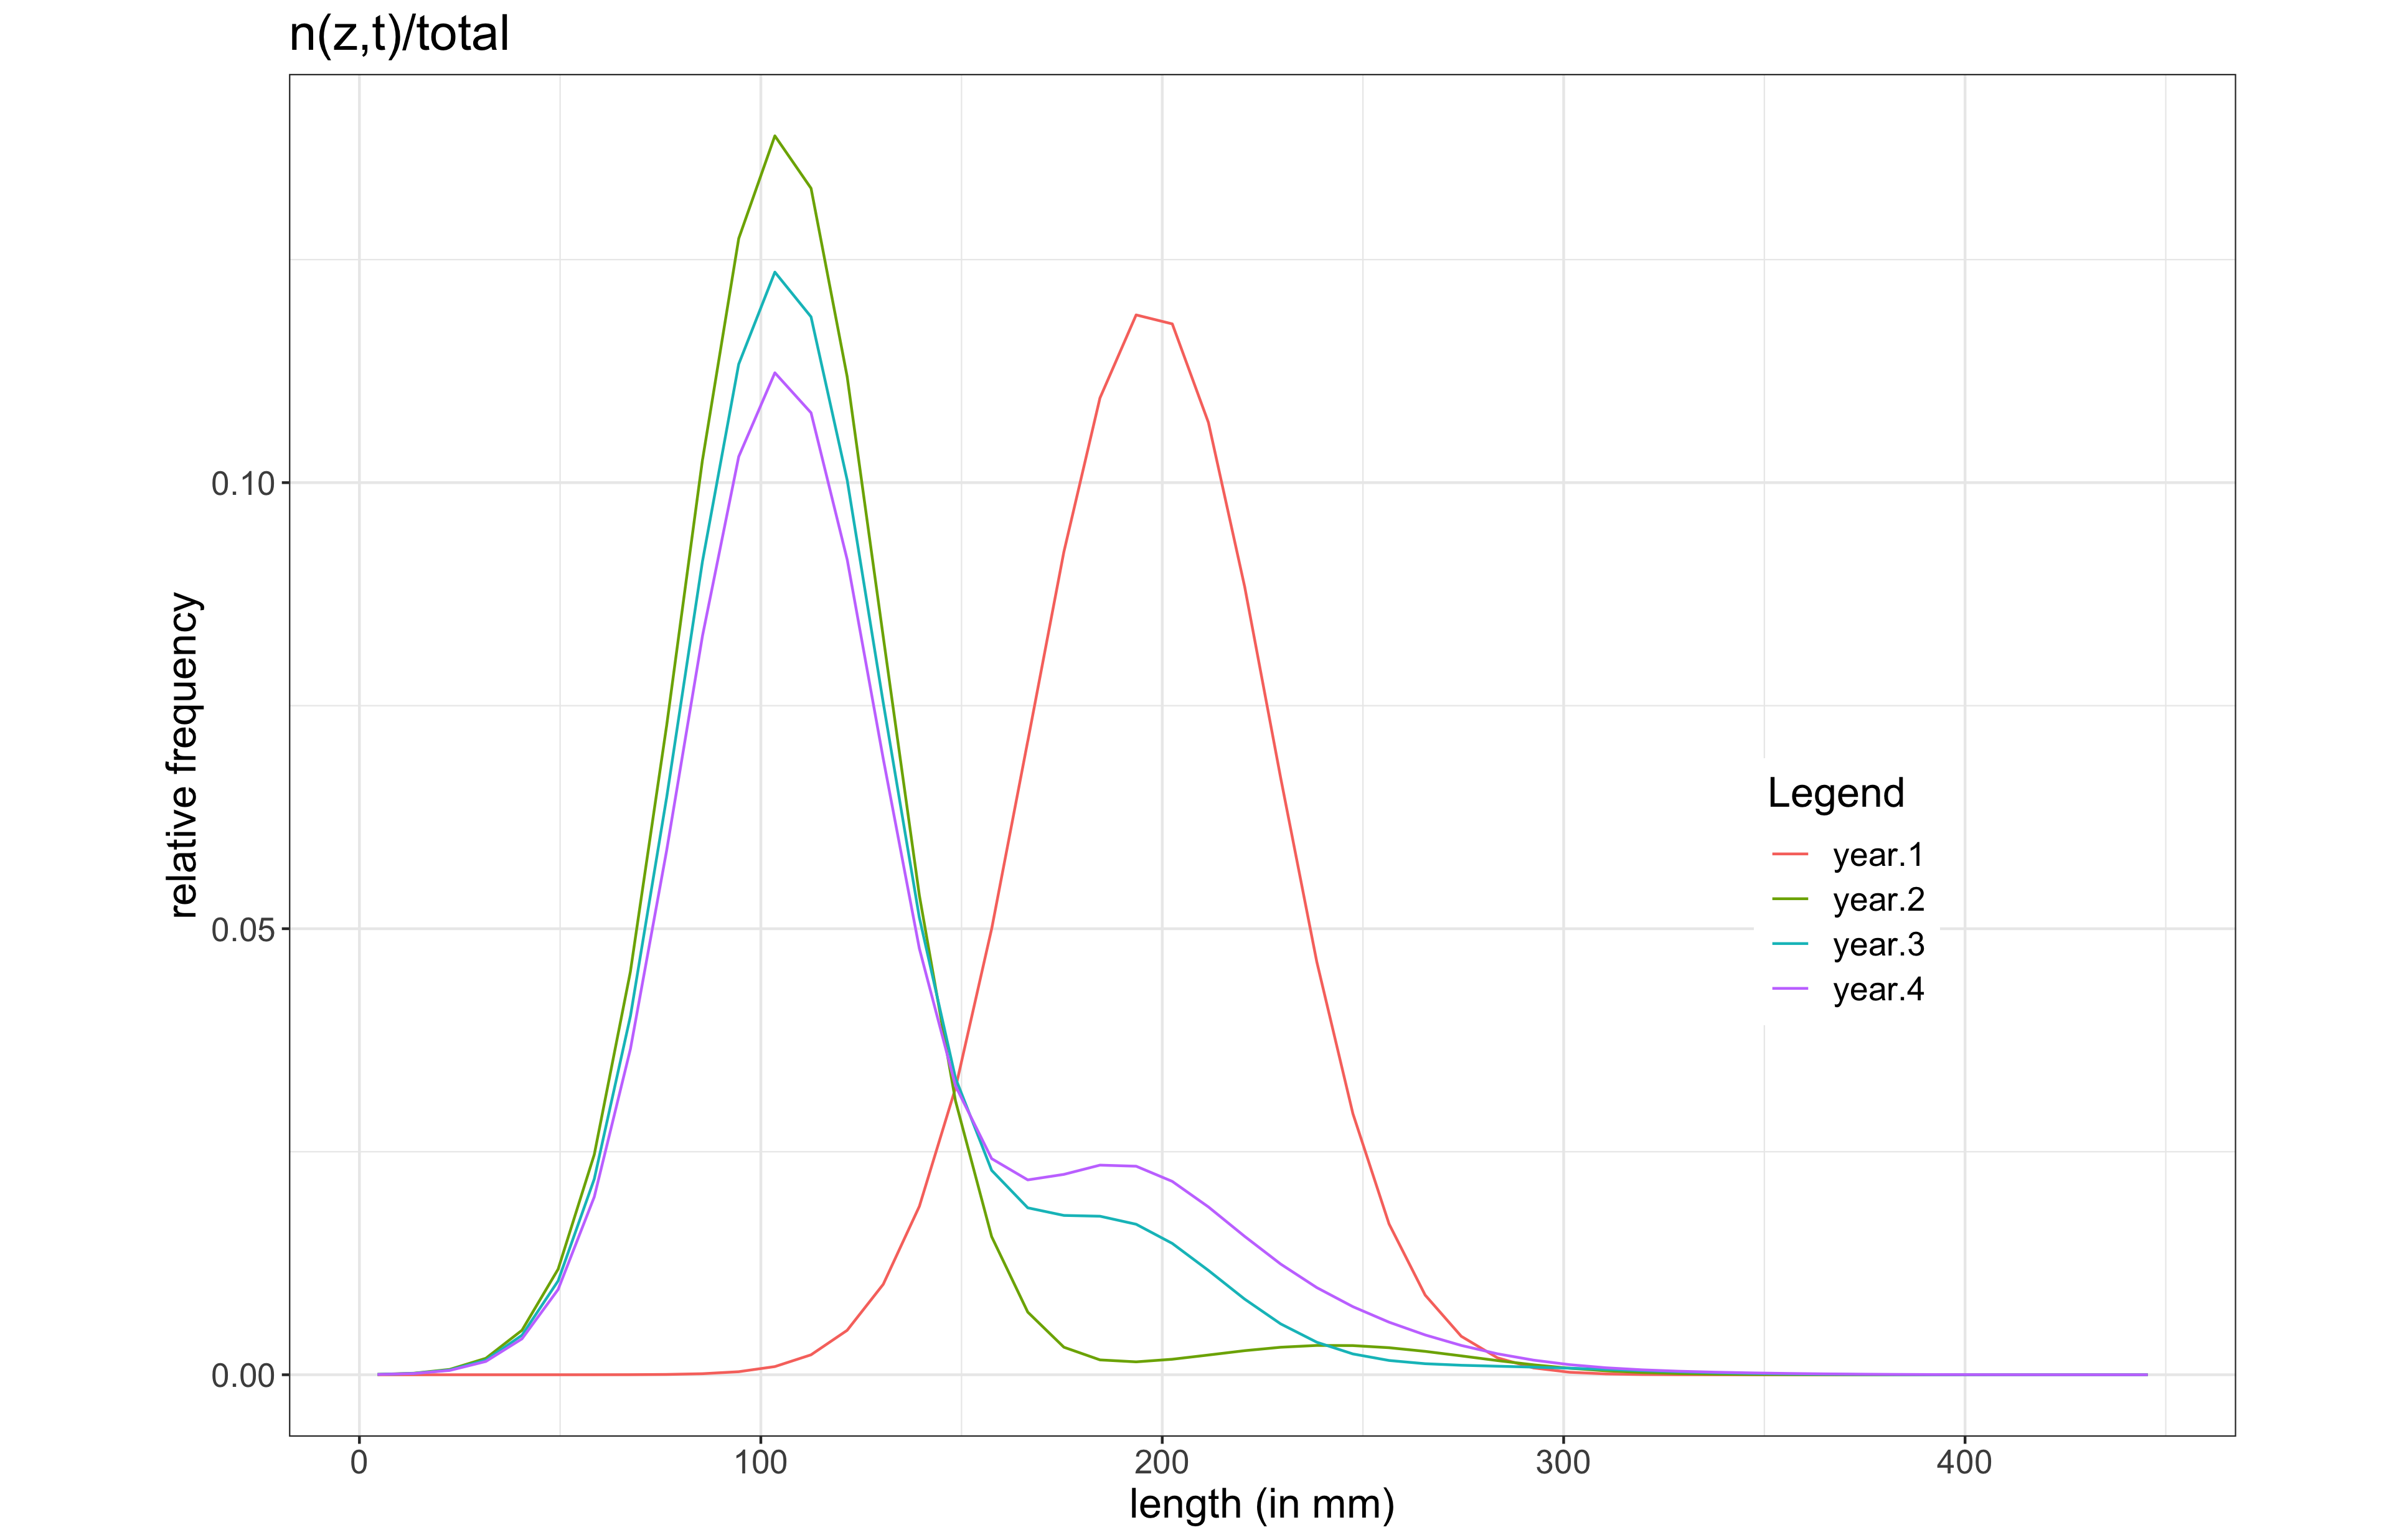
\includegraphics[width=\textwidth]{figures/sim.png}
\caption{Simulated frequency of lengths of Gizzard Shad.  Initial density  and N=xxx}
\label{fig:length_dist}
\end{subfigure}
\begin{subfigure}[b]{.43\textwidth}
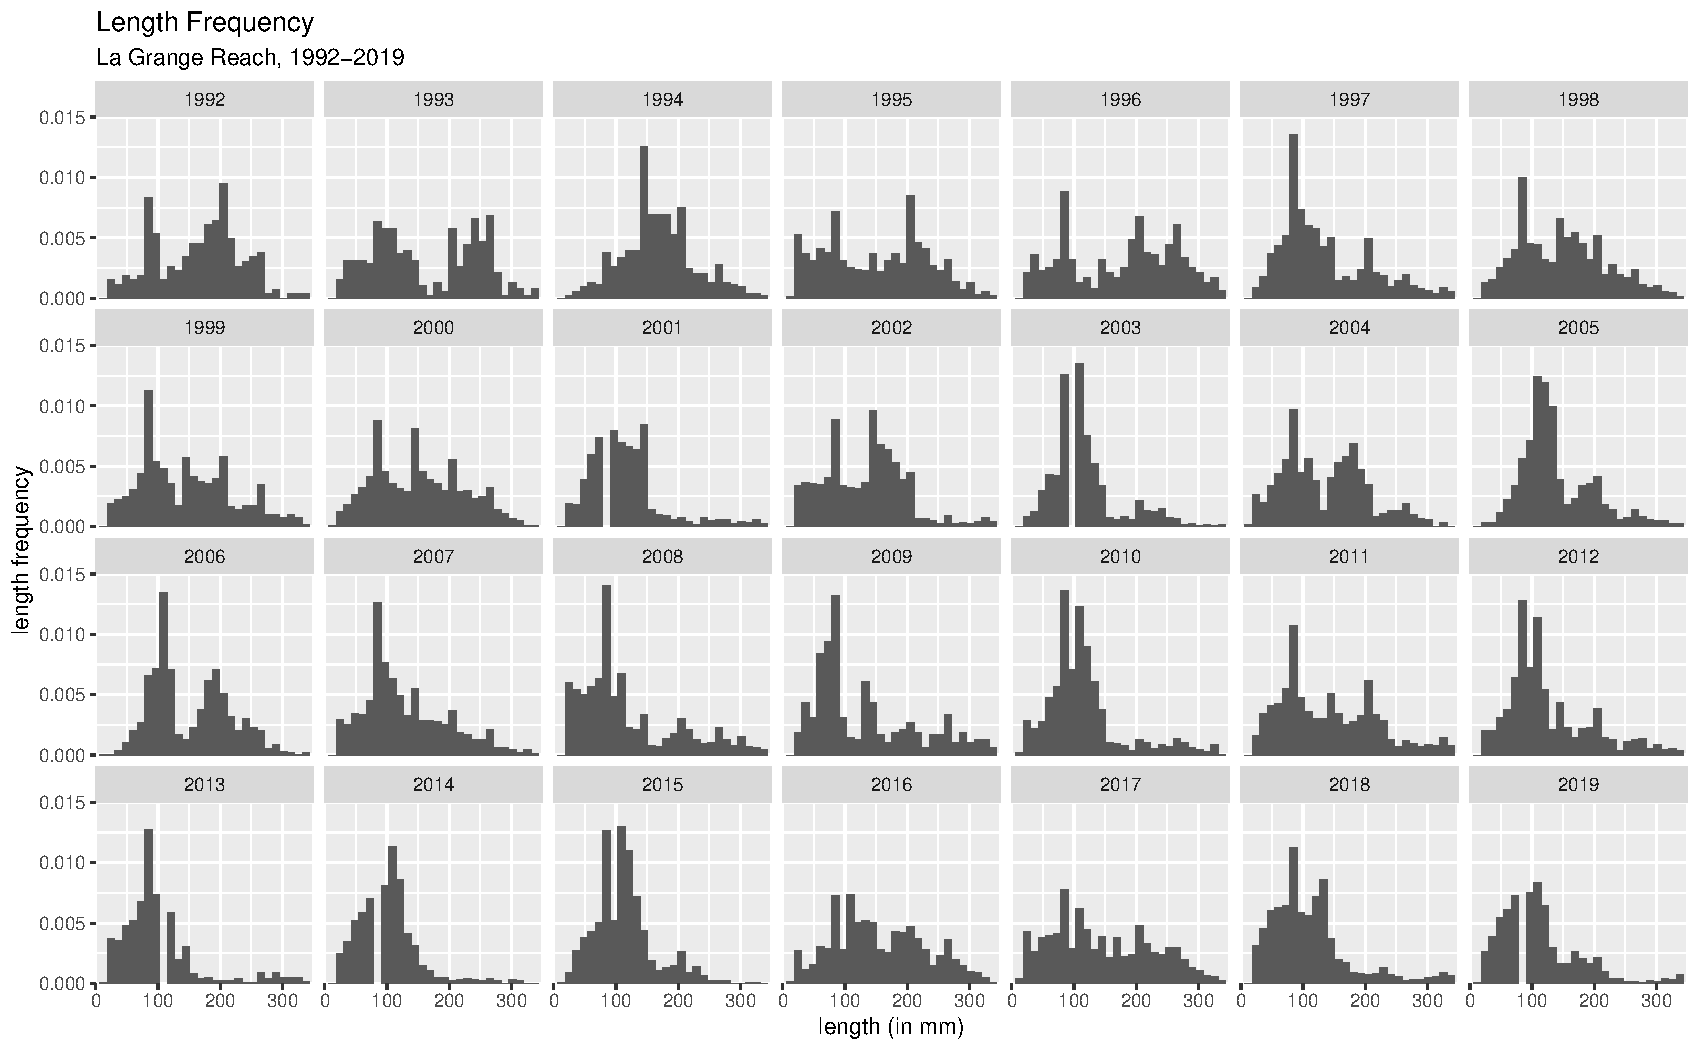
\includegraphics[width=\textwidth]{figures/LTRMgraph.pdf}
\caption{Simulated frequency of lengths of Gizzard Shad.  Initial density  and N=xxx}
\label{fig:length_dist}
\end{subfigure}
\caption{(a) Simulated length distributions. (b) LTRMP gizzard shad density from La Grange Reach 1992-2020}
%\caption{(a) Graph of $p_b(z)$ (b) Graph of $\mbox{egg}(z)$, (c) Density-dependent survival of age-0 gizzard shard.}
%\label{fig:fecundity}
\end{figure*}    




\section{Discussion}

%\begin{figure*}
%\centering
%  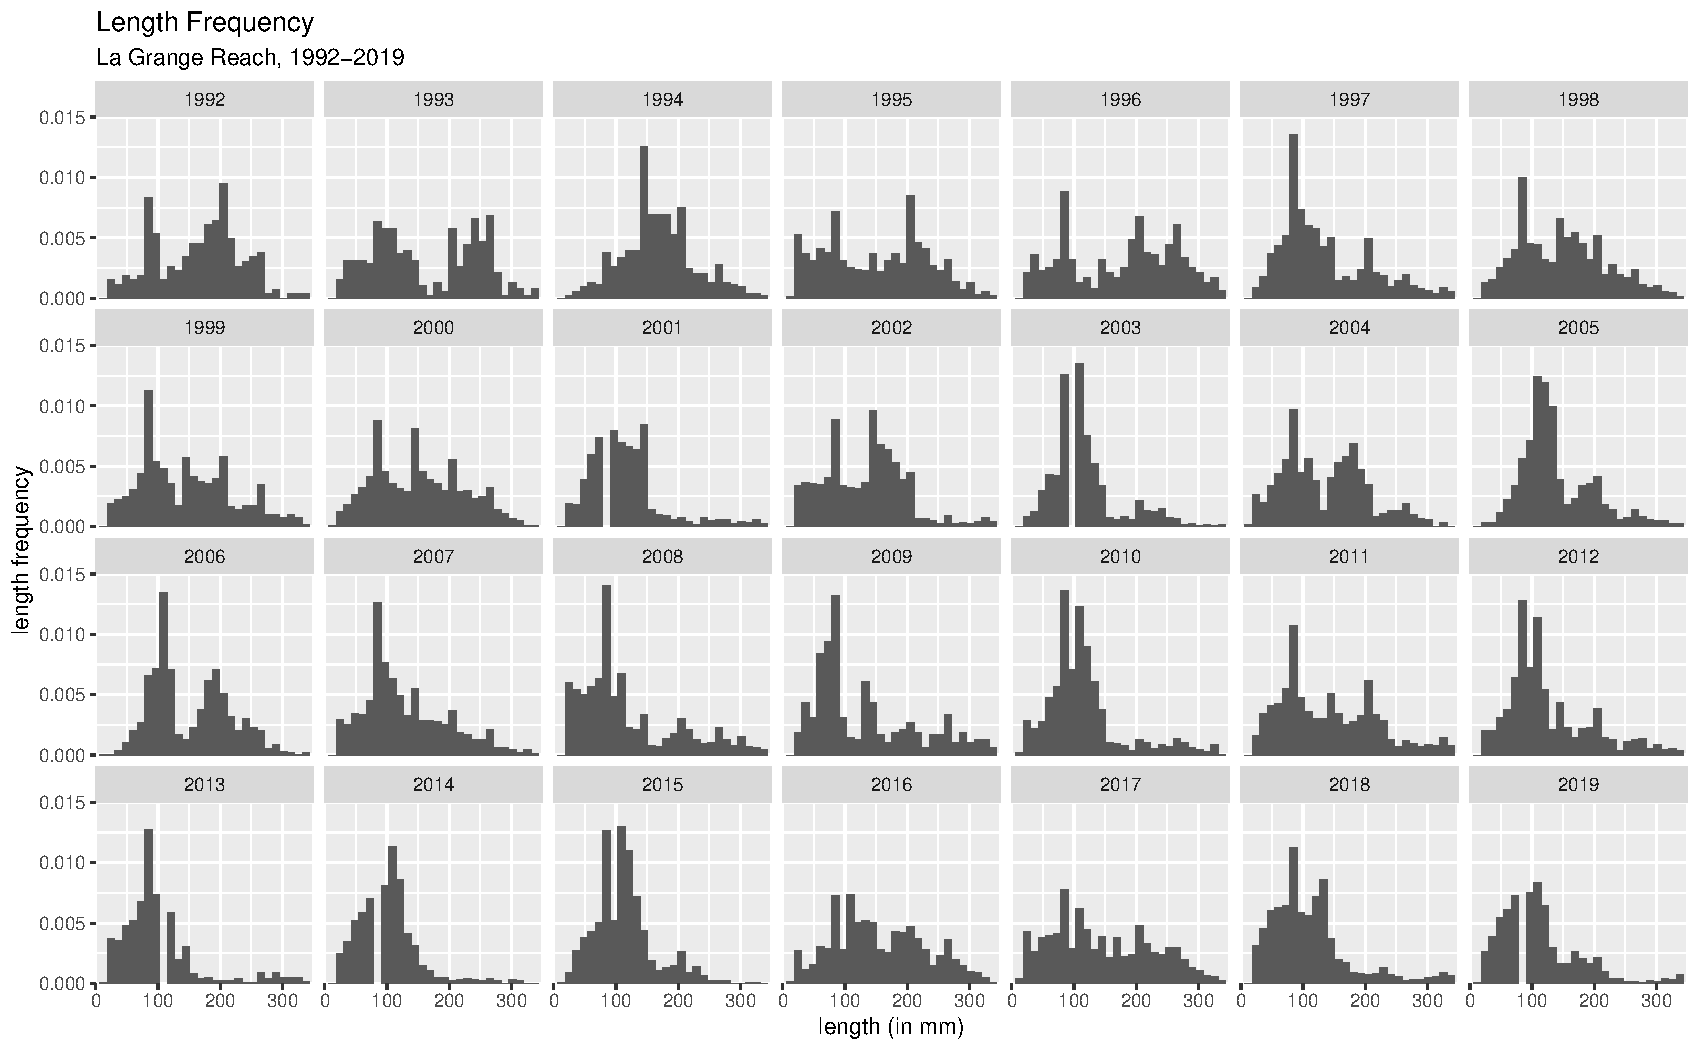
\includegraphics[width=.8\textwidth]{figures/LTRMgraph.pdf}
%\caption{LTRM}
%\label{fig:LTRM}
%\end{figure*}    

We compare a simulated length distribution with U.S. Geological Survey (USGS) Long-Term Resource Monitoring (LTRMP) data from the La Grange Reach of the Illinois River from 1992-2019. 
The La Grange Reach of the Illinois River is a 125 km segment of the lower Illinois River between the La Grange Lock and Dam at RKM 129 and the Peoria Lock and Dam at RKM 254. 
It is characterized by a wide floodplain surrounding the main channel and a mosaic of side channels, fully connected backwaters, and semi-connected backwaters.

[Comparison of Frequency plots vs Simulation - Similarities]
In these data, we see similar patterns as displayed in Figure XXX.  
Specifically, from years 2010-2012...


[Comparison of Frequency plots vs Simulation - Differences]

[Possible explanation of differences and future direction]


[More future direction - two species model]


\begin{enumerate}
\item Summary of findings and key discussion points
  \begin{enumerate}
  \item Comparison to empirical data
  \item Deviations from empirical data
  \item discussion about sameness and differences
  \item Sources of density within our model
  \end{enumerate}
\item Comparison to existing literature
  \begin{enumerate}
  \item Talk about Matt's work \citep{catalano2010size,
      catalano2011whole}
  \item Broader need for models such as this
  \end{enumerate}
\item Implications for management of species
  \begin{enumerate}
  \item Invasive species
  \item Impact of size on harvest
  \item impact of size on movement
  \end{enumerate}
\item Future ideas to explore
  \begin{enumerate}
  \item Multi-species model
  \item Spatial impacts
  \item Climate on density
  \item Changing climate scenarios
  \end{enumerate}
\end{enumerate}

\section{Acknowledgments}

These data are a product of the U.S. Army Corps of Engineer's Upper Mississippi 
River Restoration Program (UMRR) Long Term Resource Monitoring (LTRMP) element 
implemented by the U.S. Geological Survey in collaboration with the five 
Upper Mississippi River System (UMRS) states of Illinois, Iowa, Minnesota, 
Missouri, and Wisconsin.
The U.S. Army Corps of Engineers (Corps) 
provides guidance and has overall program responsibility.

We thank the U.S.~Geological Survey  Biothreats program and Great
Lakes Restoration Initiative for funding.
In addition, research was supported by NSF-DMS Grant \#1852224, ``REU Site: Ecological Modeling of the Mississippi River Basin''. 



%\subsection{Length frequencies comparison in La Grange Reach}

%\citep{delong2005upper,  mcclelland2012long}. 
%
%The USGS has sampled the fish community of the La Grange Reach of the Illinois River annually since 1993. 
%
%\begin{figure}[t] 
%  \centering
%    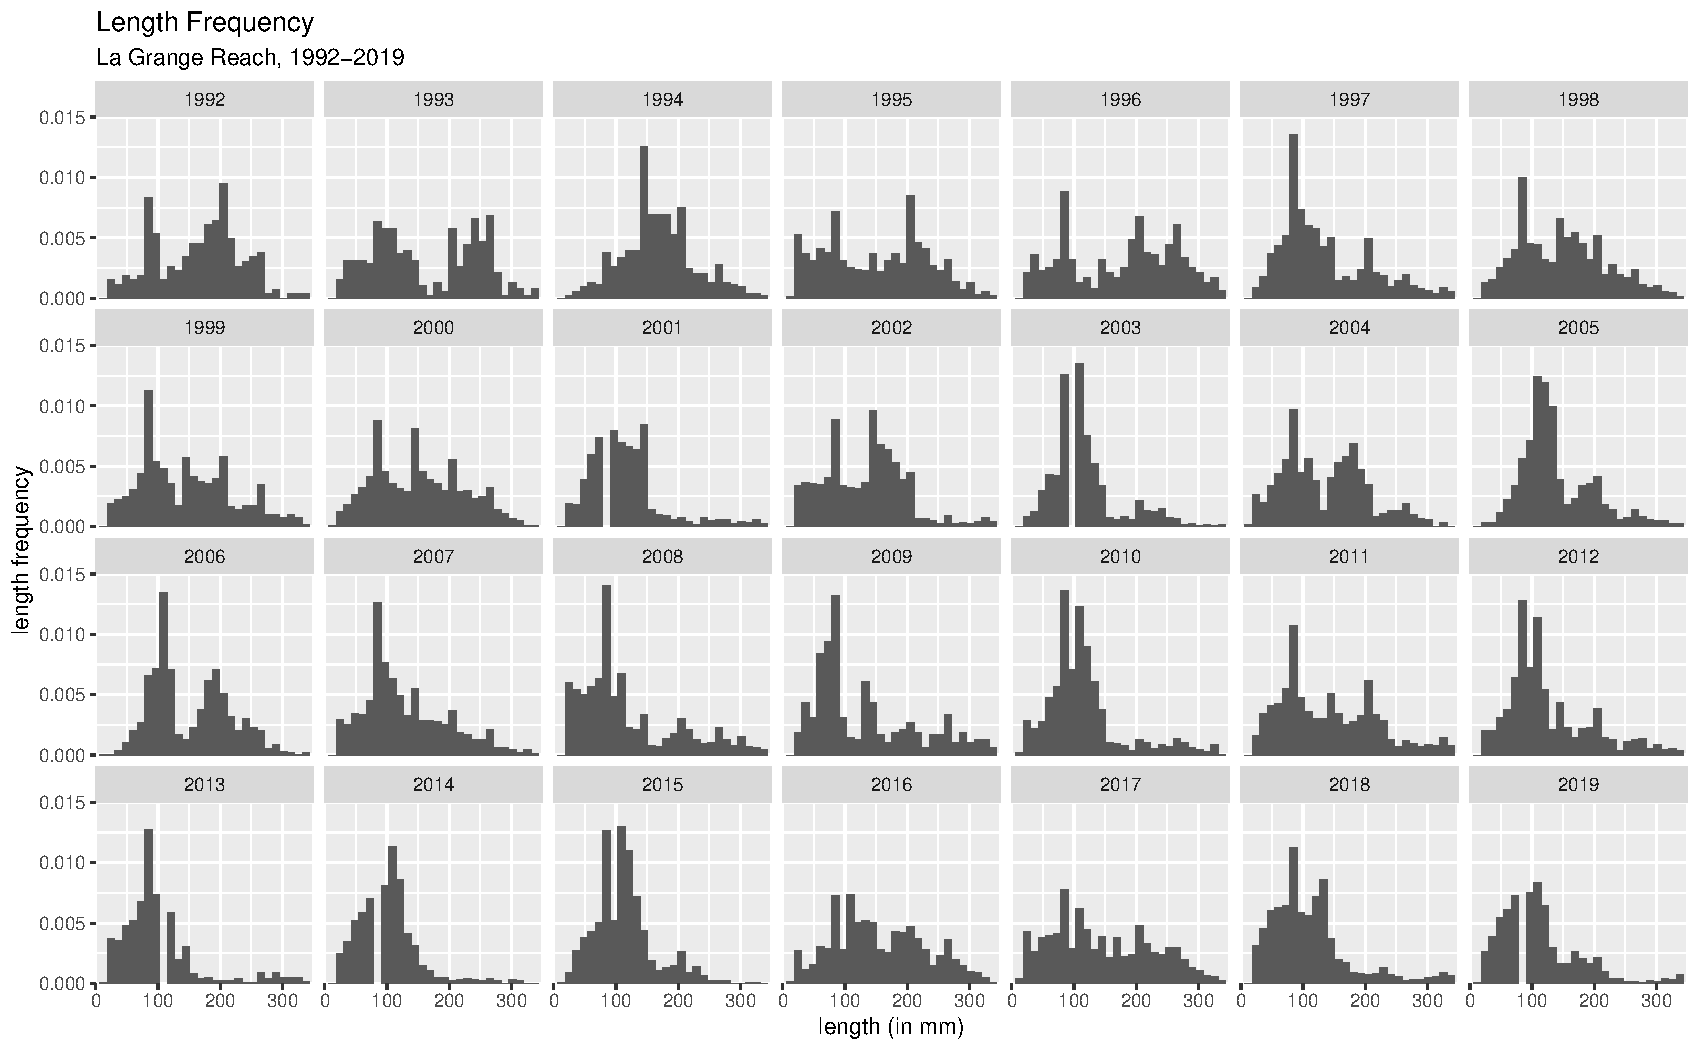
\includegraphics[width=0.5\textwidth]{figures/LTRMgraph.pdf}
%     \caption{Length frequency of gizzard shad in La Grange reach 1992-2019.}
%\label{fig:ltrm_freq}
%\end{figure}
%
%\begin{figure}[t] 
%  \centering
%    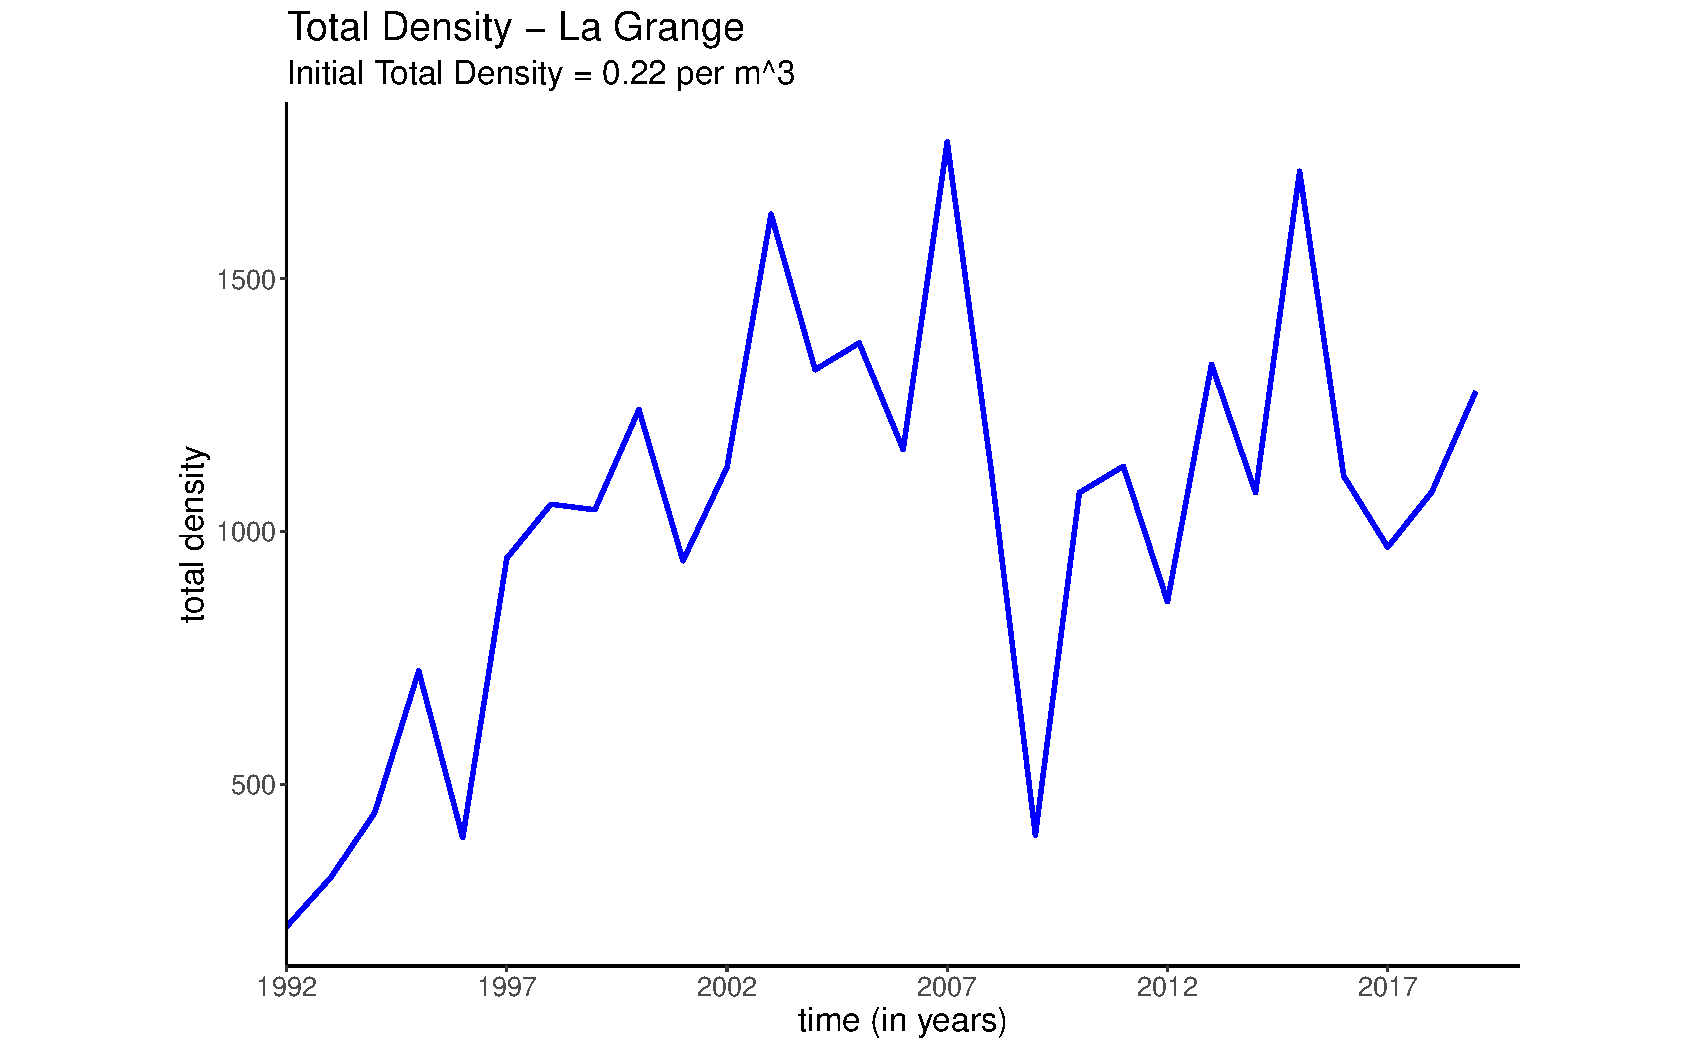
\includegraphics[width=0.5\textwidth]{figures/LTRMdensity.pdf}
%     \caption{Total density of gizzard shad in La Grange reach 1992-2019.}
%\label{fig:ltrm_freq}
%\end{figure}
%
%\begin{figure}[t] 
%  \centering
%    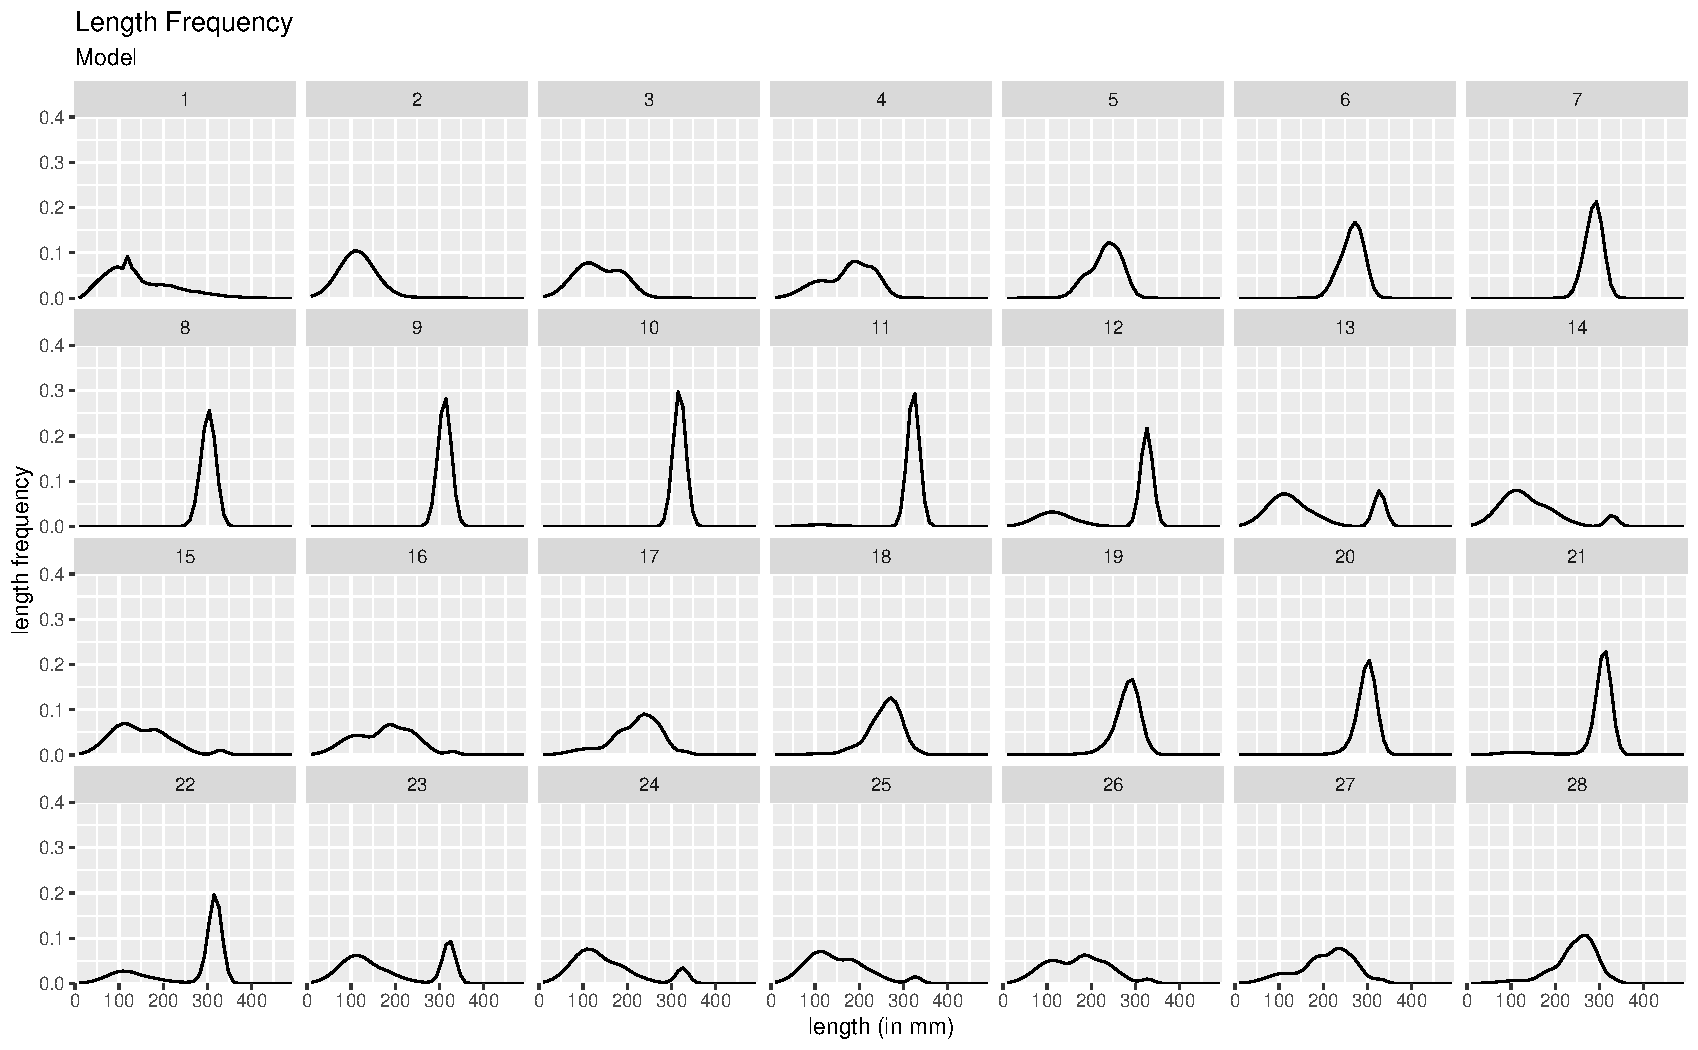
\includegraphics[width=0.5\textwidth]{figures/model_freq.pdf}
%     \caption{Simulated length frequency of gizzard shad for 28 years. Initial length frequency is the average density from LTRM data.}
%\label{fig:ltrm_freq}
%\end{figure}
%
%\begin{figure}[t] 
%  \centering
%    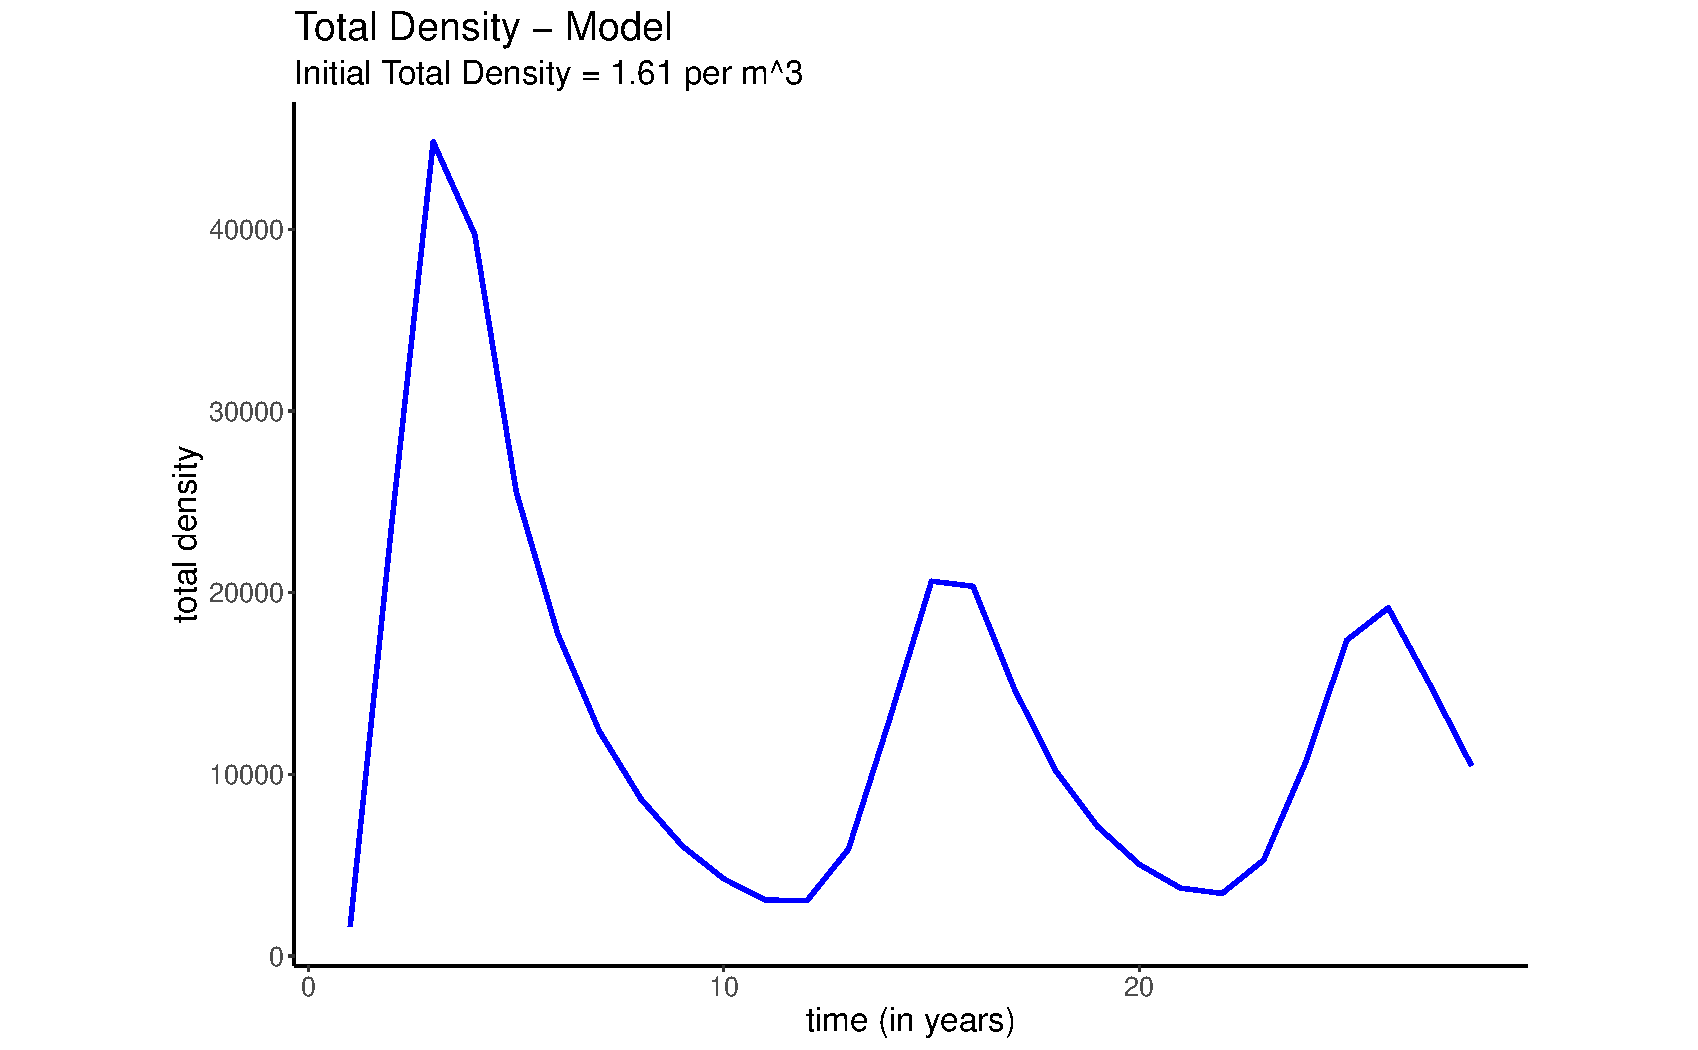
\includegraphics[width=0.5\textwidth]{figures/model_density1.pdf}
%     \caption{First 28 years of a simulated total density of gizzard shad.}
%\label{fig:ltrm_freq}
%\end{figure}
%
%\begin{figure}[t] 
%  \centering
%    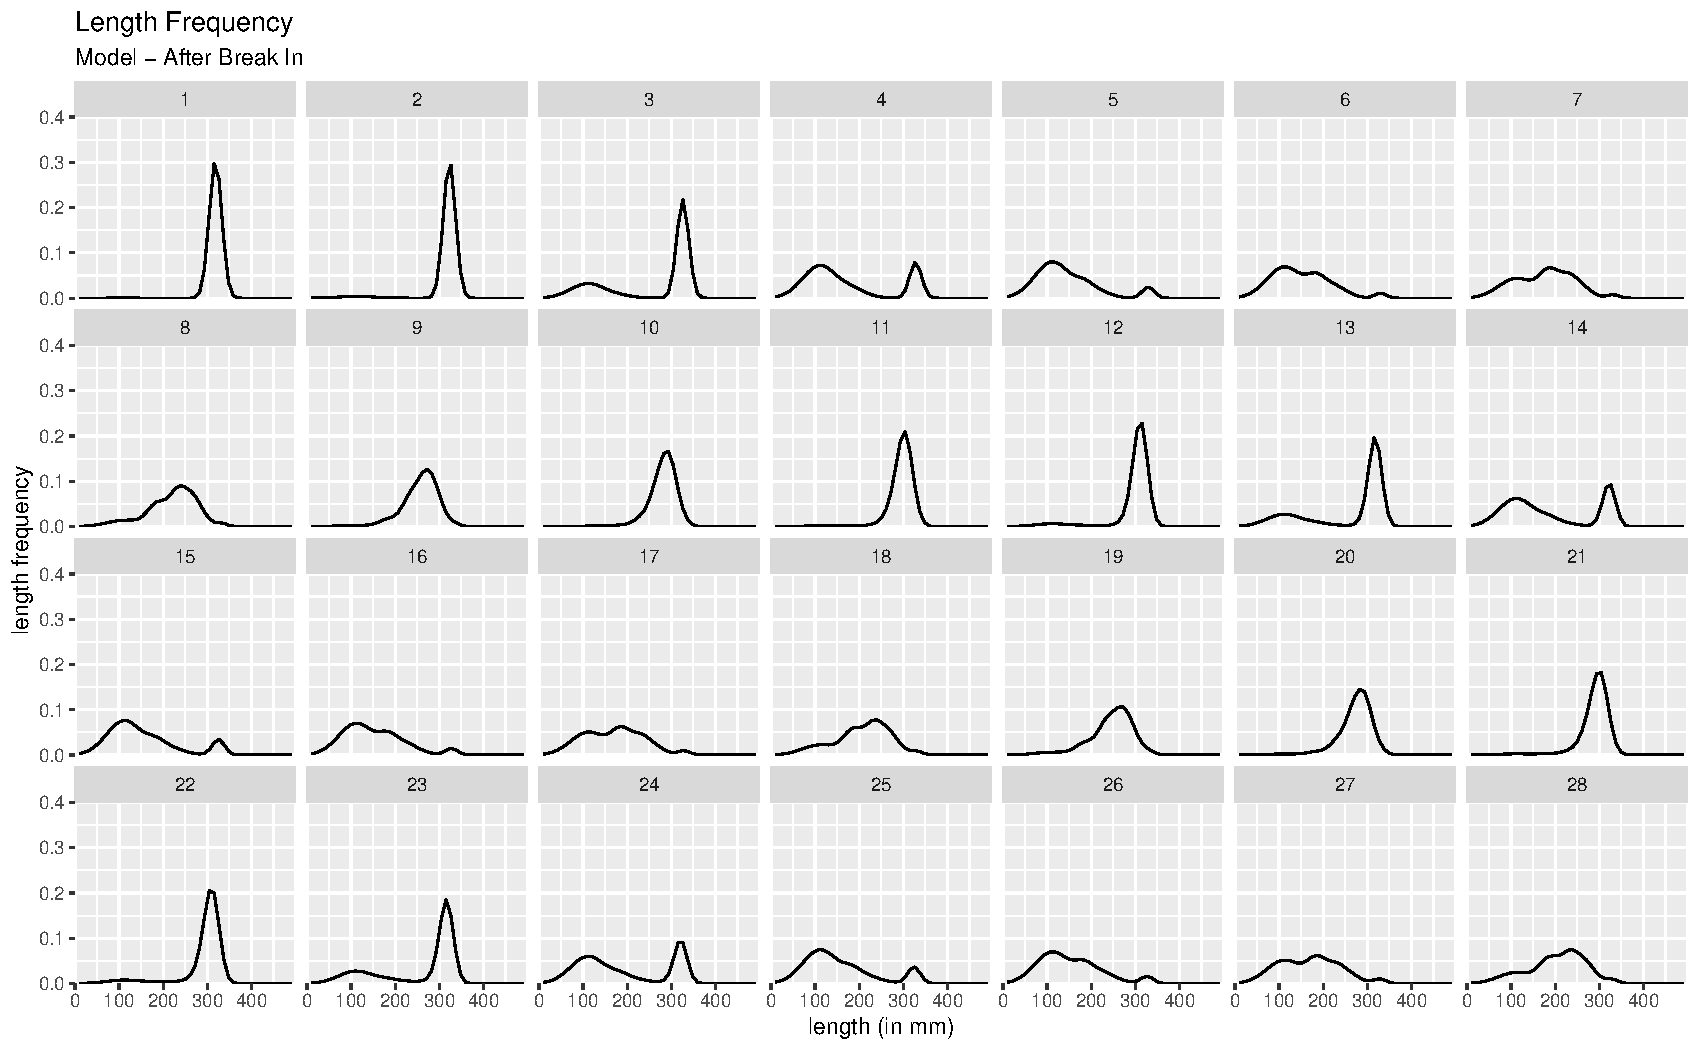
\includegraphics[width=0.5\textwidth]{figures/model_freq2.pdf}
%     \caption{Simulated length frequency of gizzard shad for 28 years. Initial length frequency is the average density from LTRM data.}
%\label{fig:ltrm_freq}
%\end{figure}
%
%\begin{figure}[t] 
%  \centering
%    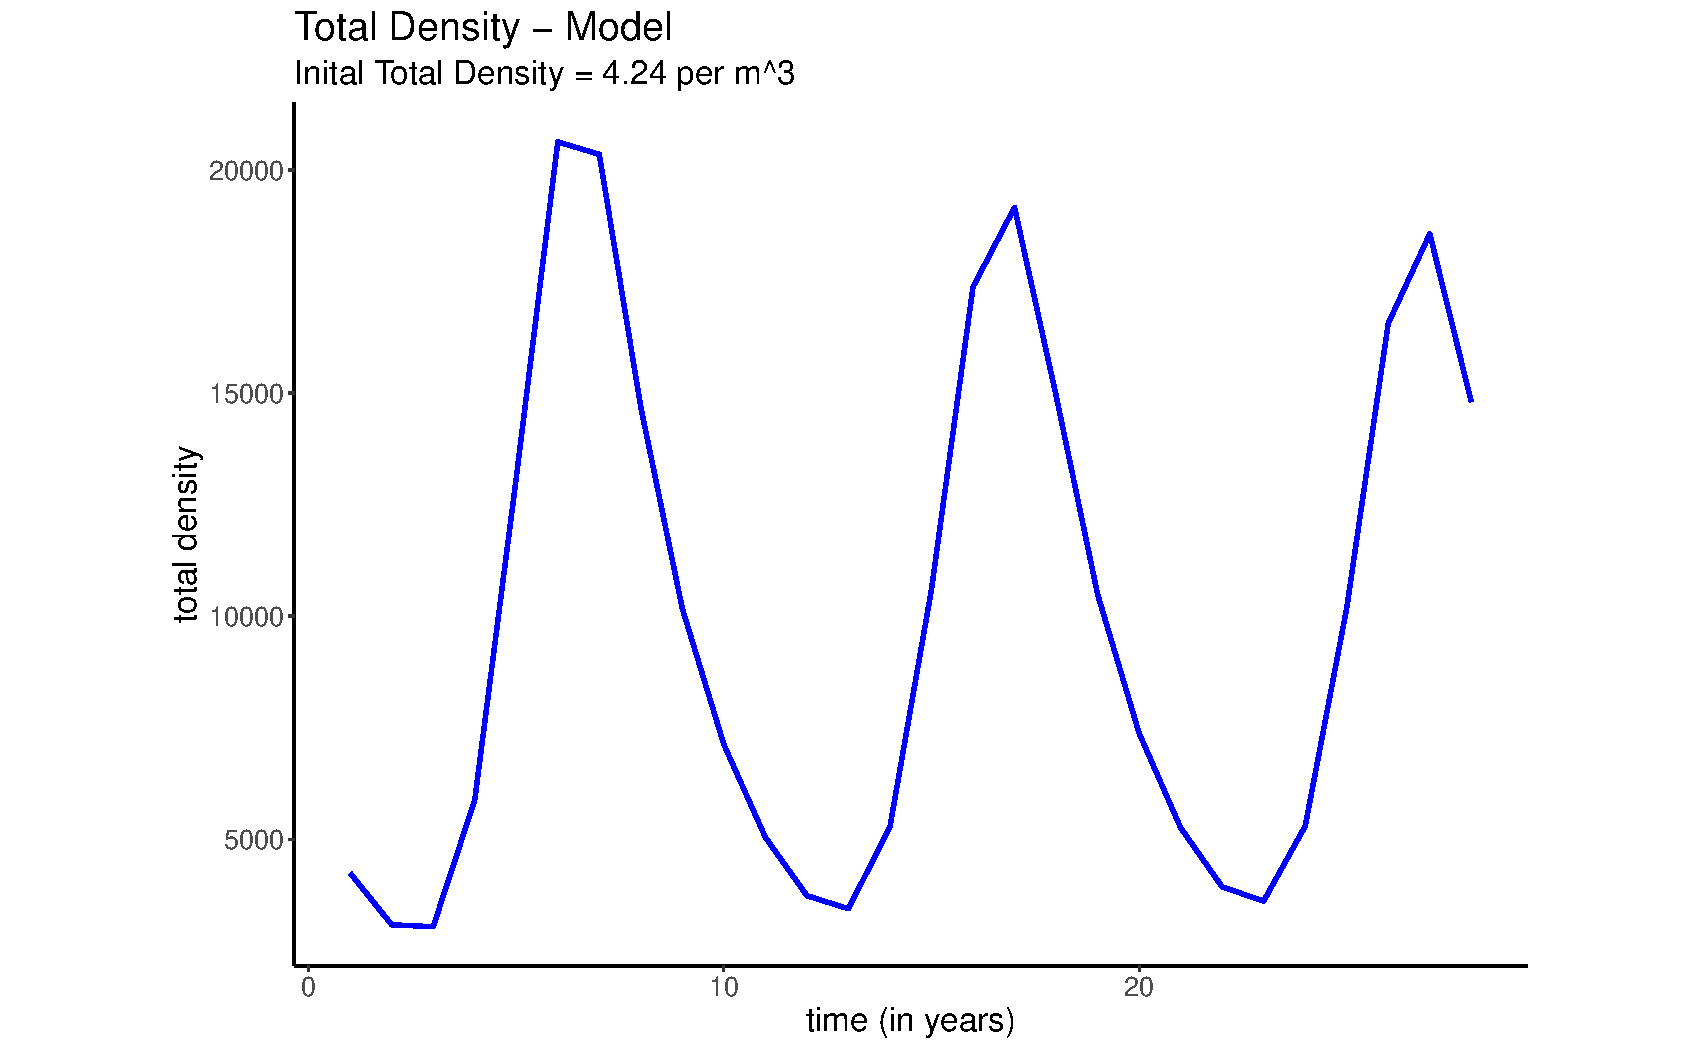
\includegraphics[width=0.5\textwidth]{figures/model_density2.pdf}
%     \caption{First 28 years of a simulated total density of gizzard shad.}
%\label{fig:ltrm_freq}
%\end{figure}
%


%Selecting years with sample sizes greater than 200 observations limited the LTMR dataset to the years 2002 and 2005. In both years, the length of the sampled gizzard shad was organized into 11 bins of equal width $\Delta z = 30\mbox{mm}$ starting with 60-90mm.  We used the 2002 length distribution to define the initial distribution $\ds n(z_i,0)$, $i=1,...,11$, as the observed values per $\Delta z$. Solving equation (\ref{eq:IPM}) with parameter values summarized in Table \label{table:parameters} for 3 years resulted in a relative distribution that is compared with the observed values in 2005 (Figure \ref{fig:LGdata_sim}).


%DISCUSS GRAPH
%
%\subsection{Total number of gizzard shad over time}
%We use the LTRM annual total catch data from the stratified random sampling sites for two sites. Fish were sampled with electrofishing used in stratified random sampling collections. 
%
%Discuss graphs
%
%\begin{figure}
%\centering
%\begin{subfigure}[b]{.32\textwidth}
%  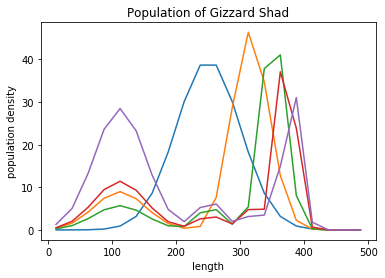
\includegraphics[width=\textwidth]{figures/popdensity.png}
%     \caption{}
%  \label{fig:popdensity}
%\end{subfigure}
%\begin{subfigure}[b]{.32\textwidth}
%   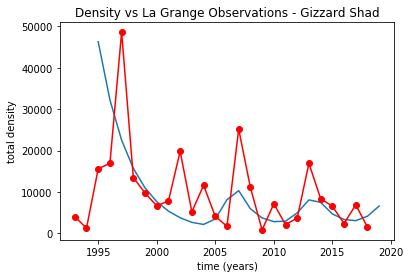
\includegraphics[width=\textwidth]{figures/lagrange.png}
%     \caption{}
%\label{fig:lagrange}
%\end{subfigure}
%\begin{subfigure}[b]{.32\textwidth}
%   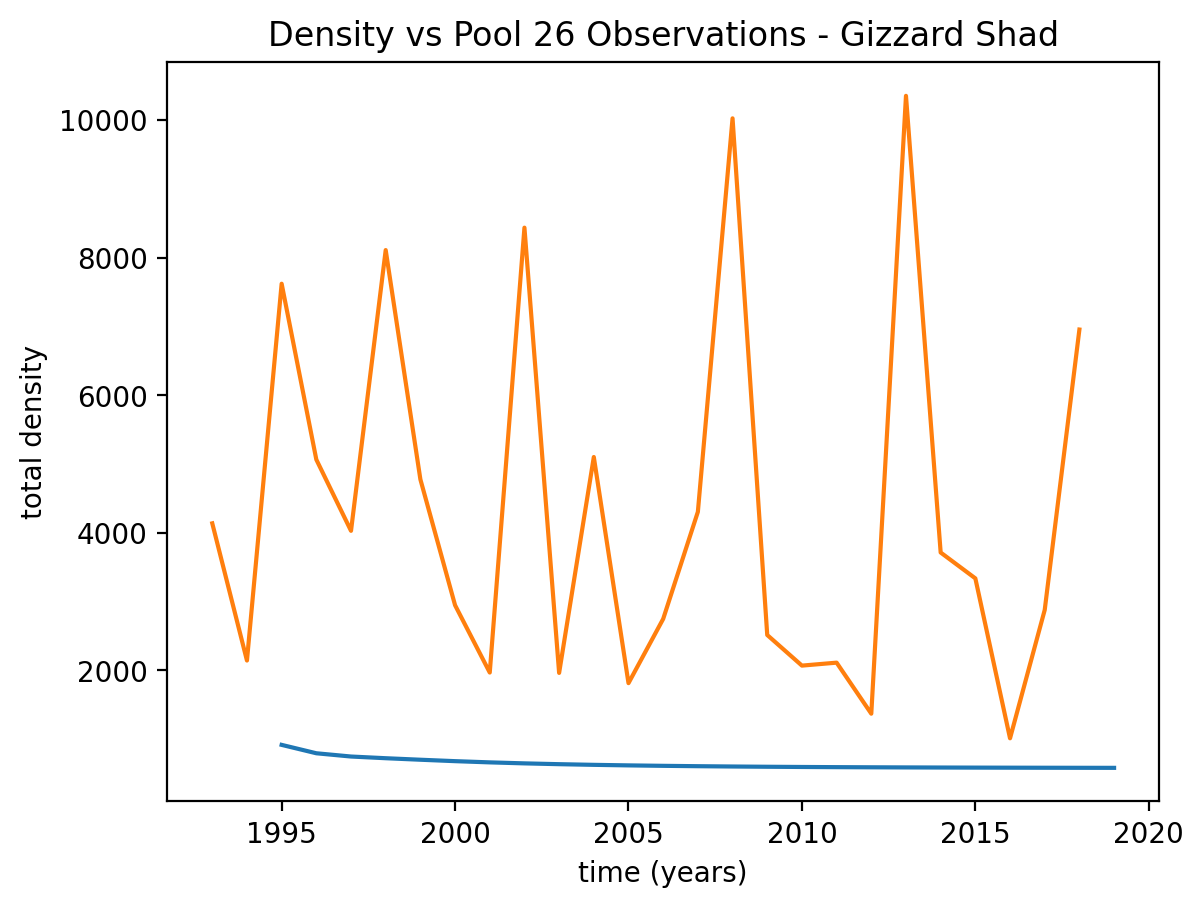
\includegraphics[width=\textwidth]{figures/pool26.png}
%     \caption{}
%\label{fig:pool26}
%\end{subfigure}
%\caption{(a) length distribution over time, (b-c) Density of gizzard shad vs La Grange reach and Pool 26 observations}
%%\caption{(a) Graph of $p_b(z)$ (b) Graph of $\mbox{egg}(z)$, (c) Density-dependent survival of age-0 gizzard shard.}
%%\label{fig:fecundity}
%\end{figure}    
%


 \bibliographystyle{elsarticle-num-names} 
 \bibliography{gizshad}



\end{document}

\endinput
%%
%% End of file `elsarticle-template-num-names.tex'.
